\pagestyle{fancy}
\chapter{NEVPT}
\label{chp:nevpt}
%\pagenumbering{arabic}

Multireference perturbation theories are important tools for the
evaluation of the correlation energy in small and medium sized molecules.
The main advantage of a perturbative approach is the reduced computational
cost when compared to a completely variational treatment, still providing a
good level of accuracy.  First attempts in deploying theoretical approaches
for MRPT are quite old\cite{rmp-39-771-1967,jcp-58-5745-1973} but these
approaches began to be mainstream only recently.

The goal of multireference perturbation theories is the creation of a quick
and accurate tool resembling the single-determinant based M{\o}ller-Plesset
(MP) approach\cite{pr-46-618-1934}, extended to a multireference context:
when the molecular system under study is well described by a
single-reference treatment, second-order M{\o}ller-Plesset perturbation
theory gives more than 90\% of the correlation energy. The zero-order
Hamiltonian is defined as the $n$ particles Fock operator 
\beq
\ham_0 = \sumonen{i} \fock(i)
\eeq
which leads to the wavefunction correction
\beq
\Psi_n^{(1)} = - \sum_{k \neq n} \ket{\Psi_k^{(0)}}
\frac{\braket{\Psi_k^{(0)}}{\perturb}{\Psi_n^{(0)}}}{E_k^{(0)} -
E_n^{(0)}}
\eeq
and to the well known second-order M{\o}ller-Plesset correction for the energy
\beq
E_0^{(2)} = - \sum_{i,j}^{\mbox{\tiny occ}} \sum_{r,s}^{\mbox{\tiny virt}} \frac{\left|
\interact{rs}{ij}\right|^{2}}{\epsilon_r + \epsilon_s - \epsilon_i -
\epsilon_j }
\eeq
where $\epsilon$ are the orbital energies associated to each orbital

Unfortunately, with a multireference zero-order wavefunction the application
of a perturbative approach is more difficult, due to the complex definition
of a zero-order Hamiltonian.  When a choice has been made, various kind of
problems arise, preventing the deployment of an easy-to-use perturbative
scheme for multireference wavefunctions. 

These problems can be accounted as the following:
\begin{itemize}
\item \textbf{lack of size consistency} (strict separability), which
requires the energy of two non-interacting systems AB to be equal to the sum
of the energies of A and B treated independently (E$_{AB} = $E$_A + $E$_B$)
\item ``\textbf{intruder states}'', when the perturbers happen to have very similar
energies to the zero-order wavefunction, leading to divergent behavior due
to the nearly zero denominator in the perturbation theory equations.
The M{\o}ller-Plesset treatment is not affected by this problem, since the
perturbers are the doubly excited determinants $\Phi_{ij}^{rs}$, and the
corresponding energies are $E_0 + \epsilon_r + \epsilon_s - \epsilon_i -
\epsilon_j$, well distinct from $E_0$.
\item \textbf{different levels of accuracy for ground and excited states}, making the
evaluation of transition energy more complex.
\item \textbf{no spin purity}, leading for example to a mix between singlet and triplet
wavefunctions. This introduces additional complexity for spectroscopical
evaluations, and spin-based property evaluations.
\item \textbf{efficiency}. The perturbative treatment is required to be fast and with
reduced disk space and memory footprints.
\end{itemize}

\subsection*{Classification of perturbative methods}

Multireference perturbation theories can be classified in two categories:
``\textit{perturb then diagonalize}'', where an effective Hamiltonian is built
and then diagonalized \cite{rmp-39-771-1967,jpa-18-809-1985}, and
``\textit{diagonalize then perturb}'', where the perturbative treatment is
applied to a variationally optimized wavefunction. 

To the latter category belong for example CIPSI techniques, started by
Huron \textit{et al.}\cite{jcp-58-5745-1973} in Paris and subsequently
developed in Pisa\cite{jcc-8-39-1987} and Ferrara
\cite{ijqc-60-167-1996,tca-98-57-1997,tca-98-117-1997,tca-105-259-2001}.
CIPSI uses single determinants as perturbers, using a baricentric
M{\o}ller-Plesset or a diagonal bielectronic
(Epstein-Nesbet\cite{pr-28-695-1926,prsl-230-312-1955}) zero-order
Hamiltonian. Although numerically efficient
\cite{ijqc-60-167-1996,tca-98-57-1997,tca-98-117-1997,jcp-83-1746-1985}, it lacks some formal
requirement, like strict separability. Other analogous methods
\cite{jcp-90-3647-1997,cpl-190-374-1992,jcp-94-5021-1991,cpl-183-443-1991, cpl-222-615-1994}
suffer from similar problems.

Another ``\textit{diagonalize then perturb}'' method is the CASPT2
approach\cite{jpc-94-5483-1990,jcp-96-1218-1992}. It makes use of contracted
perturbers obtained from a CASCI under the action of excitation operators,
and a one-electron zero-order Hamiltonian. Due to its efficiency, CASPT2 is
applicabile to large CAS spaces, providing good results for ground and
excited states at a reasonable computational cost. Integration into
the \textit{ab initio} suite \molcas makes CASPT2 one of the most used post
Hartree-Fock treatments.  The main problem of the method is its sensibility
to intruder states, leading to incorrect or divergent behavior. 

$n$-Electron Valence Perturbation Theory (NEVPT) approach
\cite{jcp-114-10252-2001,jcp-117-9138-2002,cpl-350-297-2001} is a
``\textit{diagonalize then perturb}'' method developed and implemented in
Ferrara and Toulouse. The method formally addresses both strict separability
and intruder states problems, and also comes as a natural extension to
M{\o}ller-Plesset. In fact, second-order NEVPT (NEVPT2) formally reproduces
the M{\o}ller-Plesset equations when applied to a single-reference
wavefunction.

In the development of NEVPT two levels of approximations have been
considered:
\begin{itemize}
\item the degree of contraction of the perturber space, and therefore, of
the perturber wavefunctions
\item the choice of the zero-order Hamiltonian
\end{itemize}

%nevpt single state
\section{Single-State NEVPT}

Let $\Psi_m^{(0)}$ be a zero-order CASCI wavefunction
\beq
\Psi_m^{(0)} = \sumidx{I \in \mbox{\tiny CAS}} C_{I,m} \ket{I}
\eeq
obtained diagonalizing $\ham$ inside the CAS
\beq
\proj{\mbox{\tiny CAS}}\ham\proj{\mbox{\tiny CAS}}\ket{\Psi_m^{(0)}} = E_m^{(0)} \ket{\Psi_m^{(0)}}
\eeq
where $\proj{\mbox{\tiny CAS}}$ is the projector inside the CASCI space. 

We can define perturbers in NEVPT as zero-order wavefunctions of the outer
space (external to CAS) where $k$ electrons are removed from the inactive
part and added to the valence part. If we decompose the zero-order CASCI
wavefunction as an antisymmetrized product of an inactive part (made of both
core and virtual orbitals) with $n_c$ electrons, and a valence part (made of
active orbitals) with $n_v$ electrons
\beq
\ket{\Psi_m^{(0)}} = \ket{\Phi_c \Psi_m^v}
\eeq
then the perturber wavefunctions can be expressed as
\beq
\ket{\Psi_{l,\mu}^{k}} = \ket{\Phi_l^{-k} \Psi_{\mu}^{v+k}}
\eeq
where $l$ is a collective index that describes the orbitals involved in the
operation and $\mu$ an enumerator index for the different wavefunctions. At
second order of perturbation $-2 \le k \le 2$.  

A graphical representation of the excitation scheme for NEVPT can be seen in
Fig. \ref{fig:classes}

\begin{center}
\begin{figure}[ht]
\begin{center}
\includegraphics[width=9cm,angle=270]{03_nevpt/images/classes.ps}
\end{center}
\caption{\footnotesize The eight excitation classes defining the perturber
functions in NEVPT.}
\label{fig:classes}
\end{figure}
\end{center}


The perturbers functions span a space of determinants with the same inactive
part $\Phi_l^{-k}$ and all the possible valence parts $\Psi_I^{+k}$. These
spaces are denoted as $S_l^k$
\beq
S_{l}^{k} \equiv \left\{ \Phi_l^{-k} \Psi_I^{+k} \right\}
\eeq
Perturbers will be defined in these spaces. If the full dimensionality
is exploited, the resulting approach is called \textit{totally
uncontracted}. The perturbers and their energies can be obtained by
diagonalizing the Hamiltonian inside each space
\beq
\label{eqn:teoria1_1}
\proj{S_l^k}\ham\proj{S_l^k} \ket{\Phi_l^{-k} \Psi_{\mu}^{v+k}} = E_{l,\mu}
\ket{\Phi_l^{-k} \Psi_{\mu}^{v+k}}
\eeq
however, this procedure is impractical given its high computational cost.
For each $S_l^k$ space, a diagonalization of the true Hamiltonian must be performed.

We can improve the computational asset by introducing a modified
Hamiltonian, proposed by Dyall\cite{jcp-102-4909-1995}
\beqa
\ham^D &=& \ham^D_i + \ham^D_v + C \\
\ham^D_i &=& \sum_{i}^{\mbox{\tiny core}} \epsilon_i E_{ii} +
\sum_r^{\mbox{\tiny virt}} \epsilon_r E_{rr} \\
\ham^D_v &=& \sum_{ab}^{\mbox{\tiny act}} h_{ab}^{\mbox{\tiny eff}} E_{ab} +
\frac{1}{2} \sum_{abcd}^{\mbox{\tiny act}} \integral{ab}{cd} \left( E_{ac}
E_{bd} - \delta_{bc} E_{ad} \right) \\
C &=& 2 \sum_{i}^{\mbox{\tiny core}} h_{ii} + \sum_{ij}^{\mbox{\tiny core}}
\left( 2 \integral{ij}{ij} - \integral{ij}{ji} \right) - 2
\sum_{i}^{\mbox{\tiny core}} \epsilon_i
\eeqa
where labels $i,j,\ldots$, $a,b,\ldots$, $r,s,\ldots$ denote core, active
and virtual orbitals respectively, and this convention will be retained
hereafter, $\epsilon_i$ and $\epsilon_r$ are the orbital energies of the
involved orbitals, and $E_{mn}$ operators are the spin-traced operators
$\constr{m\alpha}\destr{n\alpha} + \constr{m\beta}\destr{n\beta}$. These
operators commute with $S^2$ and $S_z$, therefore the application of these
operators on a spin-pure function produces again a spin-pure function.
Finally, the $h_{ab}^{\mbox{\tiny eff}}$ matrix evaluates as
\beq
h_{ab}^{\mbox{\tiny eff}} =  h_{ab} + \sum_j \left( 2 \integral{aj}{bj} -
\integral{aj}{jb} \right)
\eeq

$\ham^D$ behaves like the true Hamiltonian inside the CAS space, having the
same eigenvalues and eigenvectors of the true Hamiltonian projected onto the
CAS space. Also, given the decomposition for the wavefunction defined
before, the action of the Dyall's Hamiltonian can be partitioned
\beq
\ham^D \ket{\Phi_l^{-k} \Psi_{\mu}^{v+k}} = E_{l,\mu}^{k} \ket{\Phi_l^{-k}
\Psi_{\mu}^{v+k}} 
\eeq
stripping out the constant contribution of the inactive part and leaving a
subsystem to be solved for the valence part
\beq
\ham^D_v \ket{\Psi_{\mu}^{v+k}} = E_{\mu}^{k} \ket{\Psi_{\mu}^{v+k}} 
\eeq
The total energy $E_{l,\mu}^{k}$ is the sum of $E_{\mu}^{k}$ and the 
energies of the orbitals involved in the definition of the inactive part
$\Phi_l^{-k}$. This introduces the possibility to perform a single
diagonalization of the valence Dyall's Hamiltonian on the CASCI zero-order
wavefunction and evaluate the perturber energies using the property depicted
above.

\subsection*{Strongly Contracted approach}

A possible choice in the development of the NEVPT approach is to choose a
single function for each space $S_l^k$, leading to the \textit{Strongly
Contracted (SC)} scheme. A set of perturbative operators are used to produce a
single function for each space, according to the following definition
\beq
\Psi_l^k = \proj{S_l^k} \ham \Psi_m^{(0)}
\eeq
where $\proj{S_l^k}$ is the projector onto the subspace $S_l^k$. The same
result can be obtained by applying a specific part of the Hamiltonian to the
zero-order wavefunction
\beq
\Psi_l^k = V_l^k \Psi_m^{(0)}
\eeq

For each space, an appropriate operator can be devised
\beqa
V_{ijrs}^{0} &=& \gamma_{ij} \gamma_{rs} \left( \integral{rs}{ij} E_{ri} E_{sj} + \integral{rs}{ji} E_{si} E_{rj} \right) \quad i \le j, r \le s \\
V_{rsi}^{-1} &=& \gamma_{rs} \sum_a \left( \integral{rs}{ia} E_{ri} E_{sa} + \integral{sr}{ia} E_{si} E_{ra} \right) \quad  r \le s \\
V_{ijr}^{1} &=& \gamma_{ij} \sum_a \left( \integral{ra}{ji} E_{rj} E_{ai} + \integral{ra}{ij} E_{ri} E_{aj} \right) \quad  i \le j \\
V_{rs}^{-2} &=& \gamma_{rs} \sum_{ab} \integral{rs}{ba} E_{rb} E_{sa} \quad  r \le s \\
V_{ij}^{2} &=& \gamma_{ij} \sum_{ab} \integral{ba}{ij} E_{bi} E_{aj} \quad  i \le j \\
V_{ir}^{0} &=& \sum_{ab} \left( \integral{ra}{ib} E_{ri} E_{ab} + \integral{ra}{bi} E_{ai} E_{rb} \right) + h_{ri}^{\mbox{\tiny eff}} E_{ri} \\
V_r^{-1} &=& \sum_{abc} \integral{ra}{bc} E_{rb} E_{ac} + \sum_{a} h_{ra}^{\mbox{\tiny eff'}} E_{ra} \\
V_i^{1} &=& \sum_{abc} \integral{ba}{ic} E_{bi} E_{ac} + \sum_{a} h_{ai}^{\mbox{\tiny eff}} E_{ai}
\eeqa
where $\gamma_{mn} = 1 - \half \delta_{mn}$.

Auxiliary matrixes have been also defined as
\beqa
h_{mn}^{\mbox{\tiny eff}} &=& h_{mn} + \sum_j \left( 2 \integral{mj}{nj} -
\integral{mj}{jn} \right) \\
h_{mn}^{\mbox{\tiny eff'}} &=& h_{mn}^{\mbox{\tiny eff}} - \sum_b
\integral{mb}{bn}
\eeqa
The perturber functions are not normalized. The norm of these functions
\beq
N_l^k = \integral{\Psi_l^k}{\Psi_l^k} = \braket{\Psi_m^{(0)}}{
\left(V_l^k\right)^+  V_l^k }{\Psi_m^{(0)}}
\eeq
plays an important role in the Strongly Contracted development. The values
of the norms for each function are
\beqa
N_{ijrs}^{0} &=& 4 \gamma_{ij} \gamma_{rs} \left( \integral{rs}{ij}^2 + \integral{rs}{ji}^2 - \integral{rs}{ij}\integral{rs}{ji} \right) \\
%
N_{rsi}^{-1} &=& \gamma_{rs} \sum_{ab} \left[ 2 \left(\integral{rs}{ib}\integral{rs}{ia} + \integral{sr}{ib}\integral{sr}{ia} \right) \right. \nonumber \\
& & \left. - \integral{rs}{ib} \integral{sr}{ia} - \integral{sr}{ib} \integral{rs}{ia}\right] R_{ba}^{(1)} \\
%
N_{ijr}^{1} &=& \gamma_{ij} \sum_{ab} \left[ 2 \left(\integral{rb}{ji}\integral{ra}{ji} + \integral{rb}{ij}\integral{ra}{ij} \right) \right. \nonumber \\
& & \left. - \integral{rb}{ji} \integral{ra}{ij} - \integral{rb}{ij}
\integral{ra}{ji}\right] \tilde{R}_{ba}^{(1)} \\
N_{rs}^{-2} &=& \gamma_{rs} \sum_{abcd} \integral{rs}{ba} \integral{rs}{dc} R_{abcd}^{(2)} \\
%
N_{ij}^{2} &=& \gamma_{ij} \sum_{abcd} \integral{ba}{ij} \integral{dc}{ij} \tilde{R}_{abcd}^{(2)} 
\eeqa
\beqa
N_{ir}^{0} &=& \sum_{abcd} \left[ \left( 2
\integral{ra}{ib}\integral{rc}{id} - \integral{ra}{ib}\integral{rc}{di} - \integral{ra}{bi} \integral{rc}{id} \right) \braket{\Psi_m^{(0)}}{E_{ba}E_{cd}}{\Psi_m^{(0)}} \right. \nonumber \\
& & \left. + \integral{ra}{bi} \integral{rc}{di} \left( \braket{\Psi_m^{(0)}}{E_{bd}\tilde{E}_{ac}}{\Psi_m^{(0)}} + \delta_{ab} R_{ba}^{(1)}\right) \right] \nonumber\\
& & + 2 \sum_{ab} \left(2 \integral{ra}{ib} - \integral{ra}{bi} \right) h_{ri}^{\mbox{\tiny eff}} R_{ba}^{(1)} + 2 \left( h_{ri}^{\mbox{\tiny eff}}\right)^2 \\
%
N_{r}^{-1} &=& \sum_{abcdef} \integral{rd}{ef} \integral{ra}{bc} \braket{\Psi_m^{(0)}}{E_{fd}E_{eb}E_{ac}}{\Psi_m^{(0)}} \nonumber \\
&& + 2 \sum_{abcd} \integral{ra}{bc} h_{ra}^{\mbox{\tiny eff'}} \braket{\Psi_m^{(0)}}{E_{ca}E_{bd}}{\Psi_m^{(0)}} \nonumber \\
&&+ \sum_{ab} h_{ra}^{\mbox{\tiny eff'}} h_{rb}^{\mbox{\tiny eff'}} R_{ba}^{(1)} \\
%
N_{i}^{1} &=& \sum_{abcdef} \integral{ed}{if} \integral{ba}{ic} \braket{\Psi_m^{(0)}}{E_{fd}\tilde{E}_{eb}E_{ac}}{\Psi_m^{(0)}} \nonumber \\
&&+ 2 \sum_{abcd} \integral{ba}{ic} h_{di}^{\mbox{\tiny eff}} \braket{\Psi_m^{(0)}}{E_{ca}\tilde{E}_{bd}}{\Psi_m^{(0)}} \nonumber\\
&&+ \sum_{ab} h_{ai}^{\mbox{\tiny eff}} h_{bi}^{\mbox{\tiny eff}} \tilde{R}_{ba}^{(1)}
\eeqa
To evaluate these norms, the spinless density matrix of rank not higher than
three between the $\Psi_m^{(0)}$ functions are needed.  A short notation has
been used for the hole density matrixes
\beqa
\tilde{R}_{ab}^{(1)} &=& 2 \delta_{ab} - R_{ba}^{(1)} \\
\tilde{R}_{abcd}^{(2)} &=& R_{abcd}^{(2)} + \delta_{ad} R_{cb}^{(1)} + \delta_{bc} R_{da}^{(1)} - 2 \delta_{ac} R_{db}^{(1)} \\
& & - 2 \delta_{bd} R_{ca}^{(1)} - 2 \delta_{ad} \delta_{bc} + 4 \delta_{ca} \delta_{db}
\eeqa
and for the operator $\tilde{E}_{ab} = 2 \delta_{ab} - E_{ba}$

An important property of the $\Psi_{l}^{k}$ is that any other function of
the space $S_l^k$ which is orthogonal to  $\Psi_{l}^{k}$ do not interact
with the zero-order wavefunction through the true Hamiltonian. It is
possible to use the  $\Psi_{l}^{k}$ functions as a basis set for the
expansion of the first-order correction to the wavefunction, and also for
the expression of the zero-order Hamiltonian by means of a spectral
decomposition
\beq
\ham_0 = \sum_{lk} \ket{ {\Psi_{l}^{k}}' } E_{l}^{k} \bra{ {\Psi_{l}^{k}}' } +
\sum_{m}  \ket{\Psi_{m}^{(0)}} E_{m}^{(0)} \bra{\Psi_{m}^{(0)}}
\eeq
where $\ket{ {\Psi_{l}^{k}}' }$ are the normalized $\ket{ \Psi_{l}^{k} }$. 

The expression for the first-order correction to the wavefunction is
therefore
\beqa
\Psi_m^{(1)} &=& \sum_{kl} \ket{{\Psi_{l}^{k}}'}
\frac{\braket{{\Psi_{l}^{k}}'}{\ham}{\Psi_{m}^{(0)}}}{E_m^{(0)} - E_{l}^{k}} \\
&=& \sum_{kl} \ket{{\Psi_{l}^{k}}'} \frac{\sqrt{N_l^k}}{E_{m}^{(0)} - E_{l}^{k}} 
\eeqa
and for the energy is
\beq
E_{m}^{(2)} = \sum_{kl} \frac{\braket{{\Psi_{l}^{k}}'}{\ham}{\Psi_{m}^{(0)}}^2} {E_m^{(0)} - E_{l}^{k}} = \sum_{kl} \frac{N_l^k}{E_m^{(0)} - E_{l}^{k}}
\eeq
however, we still miss a definition of the perturber energies $E_l^k$.
These energies can be defined in a computationally advantageous approach, by
means of the Dyall's Hamiltonian.
\beq
E_{l}^{k} = \frac{1}{N_l^k} \braket{\Psi_{l}^{k}}{\ham^D}{\Psi_{l}^{k}}
\eeq
which leads to
\beqa
N_{l}^{k} E_{l}^{k} &=& \braket{\Psi_{m}^{(0)}}{{V_{l}^{k}}^{+} \ham^D
V_{l}^{k}}{\Psi_{m}^{(0)}} \\
 &=& \braket{\Psi_{m}^{(0)}}{{V_{l}^{k}}^{+} V_{l}^{k}
\ham^D}{\Psi_{m}^{(0)}} + \braket{\Psi_{m}^{(0)}}{{V_{l}^{k}}^{+}
\commut{\ham^D}{V_{l}^{k}} }{\Psi_{m}^{(0)}} 
\eeqa
Developing the braket and extracting the inactive part of the Dyall's
Hamiltonian we obtain
\beq
E_{l}^{k} = E_m^{(0)} + \Delta \epsilon_l + \frac{1}{N_l^k}
\braket{\Psi_{m}^{(0)}}{{V_{l}^{k}}^{+}
\commut{\ham_v}{V_{l}^{k}} }{\Psi_{m}^{(0)}}
\eeq
with $\Delta \epsilon_l$ is the sum of the orbital energies of the newly
occupied virtual orbitals minus the orbital energies of the unoccupied core
orbitals. 

The term that still need to be evaluated is the braket involving the
commutator. After development of each $V$ operator and substitution, we
obtain the contributions to the energy. Here we present the result for
$V_{rsi}^{(-1)}$:
\beqa
\braket{\Psi_{m}^{(0)}}{V_{rsi}^{(-1)}
\commut{\ham_v}{V_{rsi}^{(-1)}}}{\Psi_{m}^{(0)}} &=& \gamma_{rs} \sum_{ab}
\left[ 2 \left( \integral{rs}{ia} \integral{rs}{ib} + \integral{sr}{ia}
\integral{sr}{ib} \right) \right. \nonumber \\
&&\left. -\left( \integral{rs}{ia} \integral{sr}{ib} + \integral{sr}{ia}
\integral{rs}{ib}\right) \right] K_{ab} \nonumber \\
\eeqa
where $K_{ab}$ is analogous to a spin-free formulation of the Koopmans
matrix, defined only in the active space
\beqa
\label{eqn:koopmans_matrix}
K_{ab} &=& \half \braket{\Psi_{m}^{(0)}}{E_{as}E_{ir} \commut{\ham_v}{E_{ri}E_{sb}}}{\Psi_{m}^{(0)}} \\
&=& \sum_{c} h_{ac}^{\mbox{\tiny eff}} R_{bc}^{(1)} - \sum_{cde} \integral{cb}{ed} R_{acde}^{(2)} 
\eeqa
The contribution of the $\Psi_{rsi}^{-1}$ is therefore given by
\beq
E_m^{(2)}\left( S_{rsi}^{-1} \right) = - \frac{N_{rsi}^{-1}}{\epsilon_r
+\epsilon_s - \epsilon_i - \epsilon_{rsi}^{-1}}
\eeq
with
\beq
\epsilon_{rsi}^{-1} = \frac{1}{N_l^k}
\braket{\Psi_{m}^{(0)}}{{V_{rsi}^{-1}}^{+}
\commut{\ham_v}{V_{rsi}^{-1}} }{\Psi_{m}^{(0)}}
\eeq

An interesting case is the $V_{ijrs}^{(0)}$ case, which is identical to the
M{\o}ller-Plesset contribution 

\beq
E_m^{(2)}\left( S_{rsij}^{0} \right) = - \frac{N_{rsij}^{0}}{\epsilon_r
+\epsilon_s - \epsilon_i - \epsilon_{j}}
\eeq

NEVPT2 can therefore be seen as a generalized form of MP2 to multireference
wavefunctions, and this result is also found in the completely uncontracted
and Partially Contracted approaches\cite{cpl-317-472-2000}.

The cases involving the $V_{rs}^{-2}$  and $V_{ij}^{2}$ operators require
the knowledge of the three-particles density matrix, and the $V_{r}^{-1}$
and $V_{i}^{1}$ require auxiliary matrixes depending on the four-particles
density matrixes. All these matrixes always involve only the active indexes,
therefore represent only a minor issue for nowadays computers.

\subsection*{Partially Contracted approach}

An alternative approach, named \textit{Partially Contracted
(PC)}, is to use a subspace $\overline{S}_l^k$ of $S_l^k$.
To define this subspace, a set of functions $\Phi$ is generated by means of
the $V_l^k$ operators. These functions must be orthonormalized and purged of
linear dependencies which may arise. The resulting set spans the
$\overline{S}_l^k$ space.

Once the $\overline{S}_l^k$ spaces have been defined, we can obtain a set of
perturbers
\beq
\proj{\overline{S}_l^k}\ham\proj{\overline{S}_l^k} \ket{\Psi_{l\mu}^{k}} =
E_{l,\mu}^{k} \ket{\Psi_{l\mu}^{k}}
\eeq
where we can substitute $\ham$ with $\ham^D$ to simplify the evaluation.
Perturbers are generated by the application of the excitation operators
without contraction. For example, in the case of the $V_{rsi}^{-1}$ operator
\beq
V_{rsi}^{-1} = \gamma_{rs} \sum_a \left( \integral{rs}{ia} E_{ri} E_{sa} + \integral{sr}{ia} E_{si} E_{ra} \right) \quad  r \le s
\eeq
the Partially Contracted approach makes use of functions $\Phi_{risa} =
E_{ri} E_{sa} \Psi_m^{(0)}$ and $\Phi_{risa} = E_{si} E_{ra} \Psi_m^{(0)}$.
We can group these functions in two row vectors $\mathbf{\Phi}_{ris}$ and
$\mathbf{\Phi}_{sir}$ to write the expression of the overlap and $\ham^D$
matrixes
\beq
\integral{\mathbf{\Phi}_{ris}, \mathbf{\Phi}_{sir} }{\mathbf{\Phi}_{ris},
\mathbf{\Phi}_{sir}} = 
\left[ 
\begin{array}{cc}
2 R^{(1)} & - R^{(1)} \\
- R^{(1)} & 2 R^{(1)} 
\end{array}
\right]
\eeq
\beqa
\braket{\mathbf{\Phi}_{ris}, \mathbf{\Phi}_{sir} }{\ham^{D}}{\mathbf{\Phi}_{ris},
\mathbf{\Phi}_{sir}} & = & \left[ 
\begin{array}{cc}
2 \mathbf{K} & - \mathbf{K} \\
- \mathbf{K} & 2 \mathbf{K}
\end{array}
\right] \nonumber \\
&  & + \left( E_m^{(0)} +\epsilon_r +\epsilon_s - \epsilon_i \right)
\left[ 
\begin{array}{cc}
2 \mathbf{R}^{(1)} & - \mathbf{R}^{(1)} \\
- \mathbf{R}^{(1)} & 2 \mathbf{R}^{(1)} 
\end{array}
\right] \nonumber \\
\eeqa
where $\mathbf{R}^{(1)}$ is the one-particle density matrix in the spinless
formulation and the $\mathbf{K}$ matrix is defined as \ref{eqn:koopmans_matrix}
The diagonalization of the $\ham^D$ matrix is quickly obtained diagonalizing
$\mathbf{K}$ in the metric $\mathbf{R}^{(1)}$ to obtain $\mathbf{c}_{\mu}$ coefficients and
$\epsilon_{\mu}$ energies
\beq
\mathbf{K} \mathbf{c}_{\mu} = - \epsilon_{\mu} \mathbf{R}^{(1)} \mathbf{c}_{\mu}
\eeq
to obtain two distinct orthonormal functions
\beqa
\Psi_{ris\mu}^{-1} = \frac{1}{\sqrt{2}} \sum_{a} c_{a \mu} \left( \Phi_{risa} +
\Phi_{sira} \right) \\
{\Psi_{ris\mu}^{-1}}' = \frac{1}{\sqrt{6}} \sum_{a} c_{a \mu} \left( \Phi_{risa} -
\Phi_{sira} \right)
\eeqa
These functions will be used in the evaluation of the interaction with the
zero-order wavefunction. We define
\beqa
\left( rs, \mu i \right) &=& \braket{\Psi_{ris\mu}^{-1}}{\ham}{\Psi_{m}^{(0)}} \\
                         &=& \frac{1}{\sqrt{2}} \sum_{a} \left( \integral{rs}{ia} + \integral{sr}{ia} \right) S_{a \mu}
\eeqa
\beqa
{\left( rs, \mu i \right)}' &=& \braket{{\Psi_{ris\mu}^{-1}}'}{\ham}{\Psi_{m}^{(0)}} \\
                         &=& \sqrt{\frac{3}{2}} \sum_{a} \left( \integral{rs}{ia} - \integral{sr}{ia} \right) S_{a \mu}
\eeqa
where 
\beq
S_{a \mu} = \sum_{a'}  c_{a \mu}^{*} R_{a' a}^{(1)}
\eeq
We can now finally write the contribution for this subspace to the
second-order energy
\beq
E^{(2)}(\overline{S}_{rsi}^{-1}) = - \sum_{\mu} \frac{\left( rs, \mu
i\right)^2 + {\left( rs, \mu 
i\right)'}^2}{\epsilon_r + \epsilon_s - \epsilon_i - \epsilon_{\mu}}
\eeq


%formaldeide, acetaldeide e acetone con lara + vibrazionale
\section{Evaluation: carbonyl valence excited states}

\begin{center}
\textit{This section is based on the articles Refs. \citen{jcp-122-114304-2005} and
\citen{jms_theo-718-55-2005}} \\
\end{center}
{\ }\\

% {{{
% {{{
Small carbonyl molecules formaldehyde, acetaldehyde and acetone attracted
both experimental and theoretical chemists since long time, due to their
particular properties and roles. 

For instance the behavior of the carbonyl is important in order to describe
photochemical reactions such as Norrish type-I reactions in aliphatic
ketones and especially acetone\cite{cpc-2-273-2001,noyes-prk,pps-3-6-2004},
where the cleavage of one of the $\alpha$ CC bonds is related to an
excitation to the $S_1$ \npi\  state.  A similar kind of reaction is the
formaldehyde decomposition in \mbox{H$_2$ + CO} or \mbox{H +
HCO}\cite{arpc-34-525-1983}, mainly interesting for high-atmosphere
chemistry and astronomy.  

From the computational point of view, the small size of these systems
has allowed for a long time the application of high-level theoretical
approaches.  For these reasons, a consistent number of evaluations are
available in bibliography, defining an interesting testcase for
comparisons and discussions.

Despite these accurate insights, doubts still exist on some
photochemical features of such small molecules. For example, the absence
of a $\pi \rightarrow \pi^{*}$ transition from the experimental spectrum is
still unsolved. The first hypothesis for its absence \cite{robin-hespm}, was
that it should lie over the first ionization limit of 10.88 eV
\cite{ijmsip-1-285-1968,jacs-94-1451-1972} but it was discarded thanks to
refinements in theoretical evaluations, producing a value for this
transition in the 9.5-9.8 eV range, well below 10.88 eV.

A more probable explanation calls for a combined action of mixing between
valence states and Rydberg states (electronically excited states where the
promoted electron is described by a spatially diffuse orbital), and a very
long progression due to geometrical distortion of the excited state.  The
first effect reduces the absorption due to intensity borrowing from the $\pi
\rightarrow \pi^{*}$ to Rydberg states. The second
effect produces Franck-Condon factors with a very long and broad
progression, mainly due to the change in bond length and strength after the
excitation.  The double-bond nature changes to single-bond in the excited
state, and the resulting Potential Energy Surface along the CO stretching
coordinate is broad and with a longer CO distance with respect to the ground
state minimum. The molecule in the excited state is also highly bent along
the out-of-plane coordinate, further increasing the effect.  

As a final result, the $\pi \rightarrow \pi^{*}$ probably expresses itself in
the experimental spectrum as a broad and low-intensity band, hardly
detectable in a spectral region dominated by $n \rightarrow \mbox{Ryd}$
bands. Most of the research performed on these molecules during this thesis
was finalized to gather a deeper insight into these problems.

From a historical point of view, the most largely evaluated electronic transition
for simple carbonyl molecules is the $n_y \rightarrow \pi^{*}$ from the
oxygen lone pair. This transition is computationally very accessible, and
experimentally detectable.  For two of the three molecules under
investigation, formaldehyde and acetone, the C$_{2v}$ symmetry group forbids
this excitation, but the transition is observed due to the intensity
borrowing performed by other states interacting via vibronic coupling. For
acetaldehyde, the symmetry group is C$_s$ and the transition is
allowed by symmetry, but the local symmetry of the carbonyl determines the
selection rule and reduces the intensity\cite{jcp-87-3796-1987}.

Among the properties of excited states, the equilibrium geometrical
structures and the vibrational frequencies are also of particular interest,
since they help in the interpretation of the photochemical behavior of the
molecules and of their electronic spectra.  Within the harmonic
approximation, only the energy Hessian at the equilibrium geometry is
required for the calculation of the vibrational frequencies.  The comparison
of the theoretical frequencies so obtained with the measured ones however is
not straightforward: the anharmonicity of the potential, which is not taken
into account in the harmonic approximation, can have a sizable effect even
on the first vibrational energy difference. In the particular cases when a
series of vibrational levels for a given normal mode is experimentally
known, the ``harmonic experimental frequencies'' can be computed (see for
instance Refs. \citen{jcp-80-5968-1984} and \citen{jpc-99-13850-1995}).
These quantities can be directly compared with the theoretically computed
ones.

% }}}
\subsection*{Evaluation details}
% {{{

In this section we present various analyses performed on the valence excited
states of formaldehyde, acetaldehyde, and acetone:
\begin{itemize}
\item single state NEVPT2 study of the vertical \snpi\  and \tnpi
transitions
\item a detailed single state NEVPT2 study of $n \rightarrow \pi^{*}$, $\pi
\rightarrow \pi^{*}$  and $\sigma \rightarrow \pi^{*}$ adiabatic singlet and triplet
states
\item geometry optimization of ground and excited states at CASSCF level
\item vibrational analysis for ground and excited states at CASSCF level to
evaluate the Zero Point Energy correction
\end{itemize}

Particular care has been devoted to maintain the computational parameters as
homogeneous as possible during the evaluation, in order to perform a
systematic analysis for similarities and differences, evaluate trends and
finally allowing a deep comparison between NEVPT2 and other theoretical
methods. 

Formaldehyde, acetaldehyde and acetone have been studied using an
\mbox{ANO-1} basis set\cite{tca-77-291-1990}, contracted with the \mbox{C,O
(14s9p4d)/[4s3p1d]}, \mbox{H (8s4p)/[2s1p]} scheme. No diffuse functions have been
added in order to simplify the evaluation, removing Rydberg functions from
the orbital scheme. 

Rydberg states are expected to have a marginal influence at the equilibrium
geometry of the ground and excited valence states \cite{tca-92-227-1995}.
This is due to various factors: first, the $n \rightarrow \mbox{Ryd}$ excitations
remove an electron from a non-bonding orbital, producing Potential Energy
Surfaces nearly parallel to the Ground State surface. At the equilibrium
geometries of the valence excited states (whose minima are very
different in geometry from that of the Ground State) Rydberg states are
expected to have very high energies, making valence/Rydberg mixing
negligible. 

Second, as clearly shown by Hachey {\it et al}
\cite{jpc-99-8050-1995,jms-176-375-1996}, the perturbation of the Rydberg
states originates from a series of avoided crossings along the CO stretching
coordinate  where valence states are almost degenerate with the Rydberg ones. 
The $n \rightarrow \pi^{*}$ vertical singlet excitation is expected
around 4 eV, lower than the 8-9.5 range for the $n \rightarrow \mbox{Ryd}$
states. Valence vertical excitations laying higher in energy could be more
sensitive to Rydberg coupling in the Franck-Condon region, but the strong
dependence of valence/Rydberg mixing with respect to the geometry makes
Potential Surface alterations almost negligible when not explicitly looking
for avoided crossing situations.

We can therefore conclude that the electronic valence/Rydberg mixing is not
very influent both at the GS equilibrium geometry and at the valence excited
states equilibrium geometries, acting poorly on vertical energies, adiabatic
energies, equilibrium geometries, and harmonic vibrational frequencies.

The equilibrium geometry of the ground state (GS) and of the first three
valence singlet [\snpi, \spipi \, and \sspi] and triplet [\tnpi, \tpipi \, and
\tspi] excited states have been evaluated at CASSCF level using the \dalton
program\cite{dalton-site}. At the time of the evaluation, the development
version used for this study included an experimental direct merge of NEVPT2
into the \dalton codebase. This study also confirms the effectiveness of
this interface and its simplicity for the user.

For all compounds, the molecular skeleton in the ground state (\mbox{H-CO-H}
for formaldehyde, \mbox{C-CO-H} for acetaldehyde and \mbox{C-CO-C} for
acetone) lies in the $yz$ plane, with the carbonyl group along the $z$
axis. For acetaldehyde and acetone, the hydrogen atoms lying on the $yz$
plane are at the maximum distance from the $z$ axis. 

The symmetry group is C$_{2v}$ for formaldehyde and acetone, and C$_s$ for
acetaldehyde.  For excited state equilibrium geometries, where the molecular
skeleton is non-planar, the C$_s$ (formaldehyde and acetone) and C$_1$
(acetaldehyde) symmetry groups have been used. The motion of the CO bond
out of the CR$_2$ plane (wagging) is described by the out-of-plane bending
angle $\theta$ between the CO axis and the CR$_2$ plane. 

The active space is the same for all the states under investigation,
consisting of the involved orbitals: $n_y$ oxygen lone-pair, $\sigma$,
$\pi$ and $\pi^{*}$ CO orbitals, and $\sigma^{*}$ orbital to keep into
account the expected elongation of the carbonyl. This results in a six
electrons, five orbitals active space, hereafter called CAS(A).
The term ``$\sigma$ CO orbital'' refers to the highest occupied
molecular orbital with $\sigma$ symmetry with respect to the CO axis: at the
equilibrium geometry of the excited states this orbital can be seen as a
mixing of the $n_z$ lone pair of the oxygen atom and of the bonding
$\sigma_{\mbox{\tiny CO}}$ orbital of the GS (with a larger component on the latter).

In the case of formaldehyde and acetone, the $xz$ symmetry plane 
simplifies the definition of the active space, and preserves the nature of
this space during the symmetry break required for the geometry optimization
of the excited states. This is not true for acetaldehyde: in the evaluation
of GS and $\pi \rightarrow \pi^{*}$, the $n_y$ orbital is replaced by $n_z$,
since the latter brings a larger correlative contribution and is therefore
preferred for inclusion during the orbital optimization procedure. The
problem does not occur on evaluating the $n_y \rightarrow \pi^{*}$ excited
state, where the intrinsic electronic nature imposes the presence of the
$n_y$ orbital inside the active space.

As we saw in the previous chapter, a localized orbital approach is able to
preserve the correct nature of the active space. With a delocalized approach
this is not possible, and a different strategy is needed: to enlarge
the active space including a higher number of orbitals until a consistent
space is obtained. Adding a single doubly-occupied orbital turns out to add
a $\sigma_{\mbox{\tiny CC}}$ to the active space, and not the $n_y$ orbital. A further
increase finally includes the requested orbital in the active set and a
consistent ten electrons in seven orbitals space (named CAS(B)) is
obtained.

Finally, for comparison against the results by Dallos et
al.\cite{jcp-114-746-2001} an enriched active space has been defined for
formaldehyde, containing all the valence orbitals and electrons
[$(3-7)a_{1}$, $(1-2)b_1$ and $(1-3)b_2$] and defining a space made of 12
electrons in ten orbitals (named CAS(C)). 

As pointed out in Refs. \citen{mp-101-1937-2003} and
\citen{cpl-371-49-2003}, for a given choice of the active space multiple
different final solutions exist. The difference resides in the nature of
the orbitals included inside the active space, and it hardly affects the
equilibrium geometries obtained after a geometry optimization.  In order to
produce a consistent behavior, during the optimization of the ground and
excited states a proper nature of the active space has been kept.  It is
important to note that this choice does not always match the minimum energy
criterion.

Both Strongly and Partially contracted NEVPT have been applied
for the evaluation of the excitation energies, involving all electrons and
orbitals in the perturbative treatment.  Vertical excitation energies have
been evaluated computing the electronic energy of all states at the CASSCF
equilibrium geometry for the ground state. For adiabatic excitation
energies, the single state CASSCF equilibrium geometry for the appropriate
excited state has been considered.

The vibrational frequencies have been computed analytically using the
harmonic approximation and are here reported without any scaling factor. The
normal mode assignment has been done looking at the dominant contributions
of the atom displacements.  From the knowledge of the harmonic frequencies,
the Zero Point Energy (ZPE) has been obtained at CASSCF level, and kept into
account in this form for both CASSCF and NEVPT evaluations.  This introduces
the approximation that NEVPT acts on the states with a pure translation of
the CASSCF energy surface, not altering the shape (which in turn acts on
the Zero Point Energy).

% }}}

\subsection*{Results and discussion}
\subsubsection*{Ground state}
% {{{

CASSCF optimized geometries for the ground state are reported in Tab.
\ref{tbl:gs_geometries}. 
\begin{center}
\begin{threeparttable}
\footnotesize
\begin{tabular*}{0.80\textwidth}{lccccc}
\hline
Method 						& $R_{\mbox{\tiny CO}}$	& $R_{\mbox{\tiny
CH}}$\tnote{a} & $R_{\mbox{\tiny CC}}$ & $\angle \mbox{XCY}$\tnote{b} 	& $\angle \mbox{OCC}$ \\	
\hline
\multicolumn{6}{c}{\small Formaldehyde} \\
CASSCF[CAS(A)]\tnote{c} 	& 1.220		& 1.090				& 			& 117.3					&       	 \\
CASSCF[CAS(C)]\tnote{c}		& 1.210		& 1.118				& 			& 115.1					&       	 \\
Exp.\cite{jpsj-18-1174-1963}& 1.208		& 1.116				& 			& 116.5					&       	 \\
\multicolumn{6}{c}{\small Acetaldehyde} \\                                                     
CASSCF[CAS(B)]\tnote{c}		& 1.222		& 1.092				& 1.501 	& 116.3					& 124.2   	 \\
Exp.\cite{jpc-8-619-1979}	& 1.213		& 1.106				& 1.504		& 114.9					& 124.0    	 \\
\multicolumn{6}{c}{\small Acetone} \\                                                          
CASSCF[CAS(B)]\tnote{c}		& 1.224		& 					& 1.509 	& 117.2					& 121.4   	 \\
Exp.\cite{jms-18-344-1965}	& 1.222		&      				& 1.507		& 117.1					& 121.4    	 \\
\hline
\end{tabular*}
\caption{\footnotesize Formaldehyde, acetaldehyde and acetone ground state
equilibrium geometries.  Distances in \AA, angles in
degrees.\label{tbl:gs_geometries}}
\begin{tablenotes}
\footnotesize
\item[a] In acetaldehyde, H is the aldehydic hydrogen.
\item[b] Formaldehyde X=H, Y=H; acetaldehyde X=H, Y=C; acetone X=C, Y=C.
\item[c] This work.
\end{tablenotes}
\end{threeparttable}
\end{center}

% jms-120-118-1986 ?

\vspace{5mm}
An overall agreement with the experimental data can be appreciated. For
formaldehyde, the CAS(A) bond distances show a discrepancy with respect to
the experiment of 0.012 $\AA$ (R$_{\mbox{\tiny CO}}$) and
0.026 $\AA$ (R$_{\mbox{\tiny CH}}$). The error for the HCH angle is of $0.8^{\circ}$. The
CAS(C) produces values in even better agreement, with the exception of the
HCH angle value which is higher ($1.4^{\circ}$) than with CAS(A) but remains small.

In the case of acetaldehyde and acetone, it is possible to note that the
carbonyl group maintains the same structure found in formaldehyde, and both
CASSCF values agree with the experimental data.
% }}}
\subsubsection*{General consideration on the excited states}
% {{{
An extended review of the experimental works on excited states of
formaldehyde has been presented by Moule and Walsh\cite{cr-75-67-1975} and
Clouthier and Ramsay\cite{arpc-34-31-1983}. Many theoretical works have been
dedicated to formaldehyde, starting from the works of Whitten and
Hackmeyer \cite{jcp-51-5584-1969} and of Buenker and Peyerimhoff
\cite{jcp-53-1368-1970}. In 1982 a review of these pioneering theoretical
works was published \cite{davidson-es}. More recently the EOM-CCSD
\cite{cpl-241-26-1995,cpl-248-189-1996}, EOM-MBPT \cite{cpl-248-189-1996},
TDDFT/B3LYP \cite{cpl-297-60-1998}, TDDFT/PBE0 \cite{jcp-111-2889-1999},
OO-CCD \cite{jcp-113-6509-2000}, CASPT2 \cite{tca-92-227-1995}, MRD-CI
\cite{jpc-99-8050-1995,jpc-99-16576-1995}, MRCISD+Q \cite{tca-106-369-2001},
MRAQCC/LRT \cite{tca-106-369-2001}, \\ MRPT2 \cite{cpl-296-435-1998},
MR-CI \cite{mp-100-1647-2002}, (SC)$^2$-MR-SDCI \cite{mp-101-483-2003},
CCSD\cite{mp-101-483-2003}, and NEVPT2 \cite{tca-111-352-2004} have been
applied to formaldehyde, mainly focusing on vertical transitions.

Acetone has been less studied from the theoretical point of view. Most of
the existent investigations concentrated on the \snpi\ state
\cite{jms_theo-365-29-1996,jms_theo-401-29-1997,jcp-110-62-1999,jcp-111-205-1999,cpl-337-331-2001},
or on the vertical transition energies
\cite{tca-111-352-2004,cpl-241-26-1995,cpl-297-60-1998,jcp-104-1791-1996,jpca-106-4192-2002}.
The S$_1$ and T$_1$ surfaces have been also investigated
\cite{cpc-2-273-2001,cpl-284-19-1998,cpl-325-86-2000,cpc-3-57-2002} because
of the already cited Norrish type-I reaction, which takes place on these surfaces.
In this reaction, after the excitation to the S$_1$ state, the molecule
dissociates leading to the cleavage of one of the $\alpha$-CC bonds. For the
${}^1(\pi \rightarrow \pi^{*})$ state, only one determination of the
equilibrium geometry exists \cite{cpc-3-57-2002}.  Concerning the $\sigma
\rightarrow \pi^{*}$, no studies have been performed.

Finally, for acetaldehyde the theoretical studies of the valence states are
even more scarce than for acetone.  From the theoretical point of view,
CIS-MP2 \cite{jpc-97-4293-1993}, UMP2  \cite{jpc-98-1519-1994,jms_theo-315-9-1994}, CIS(D) \cite{cpl-219-21-1994},
EOM-CCSD \cite{cpl-241-26-1995}, P-EOM-MBPT \cite{cpl-248-189-1996}, TDDFT
\cite{jcp-108-4060-1998,cpl-297-60-1998} studies have been recently published, but only in
few cases the geometrical structure and the frequencies of the excited
states have been investigated.  

Despite the large number of theoretical works on these three molecules,
various valence states have never been characterized and even for the states
considered a study of all the molecules based on a common strategy appears
to be missing. The use of different theoretical approaches, for which
different approximation levels have been employed, makes it difficult to 
compare the data reported in the literature.

% }}}
\subsubsection*{The vertical \npi\  states}
% {{{
The calculation of the \npi\  singlet and triplet vertical 
energies are presented in Tabs. \ref{tbl:vertexc_form_npi},
\ref{tbl:vertexc_aceta_npi} and \ref{tbl:vertexc_aceto_npi} for
formaldehyde, acetaldehyde and acetone, respectively.  All the NEVPT2
vertical excitation energies agree with the previously published high-level
theoretical results. 

In the case of the singlet state of formaldehyde a fairly large number of
different theoretical works has been published, and experimental values
exist. For this state the NEVPT2 results (4.00-4.08~eV) are very close to
the best available theoretical data, which are in the range 3.90-4.10~eV and
with one of the experimental values (4.07~eV).

The valence triplet state has been less studied computationally, while
experimental information exists.  The NEVPT2 computed values for this state
agree well with the available data, the only relevant differences being with
TDDFT/B3LYP\cite{cpl-297-60-1998} and RMS MRPT2/IVO\cite{cpl-296-435-1998}
which, however, show too low and too high values, respectively.
The tendency of TDDFT to give a too low transition energy for the \tnpi\
state has been found also in a TDDFT/PBE0 study\cite{jcp-111-2889-1999}
(3.18 and 3.20 eV with two basis sets).

\begin{center}
\begin{threeparttable}
\footnotesize
\begin{tabular*}{0.80\textwidth}{l@{\hspace*{27mm}}cc}
\hline
Method                  &   \snpi & \tnpi\\
\hline                                   
CASSCF  (CAS(A))\tnote{a} &    4.37 & 3.99 \\
NEVPT2 SC (CAS(A))\tnote{a} &    4.02 & 3.59 \\
NEVPT2 PC (CAS(A))\tnote{a} &    4.00 & 3.56 \\
CASSCF  (CAS(C))\tnote{a} &    4.51 & 4.25 \\
NEVPT2 SC (CAS(C))\tnote{a} &    4.08 & 3.69 \\
NEVPT2 PC (CAS(C))\tnote{a} &    4.06 & 3.66 \\
NEVPT2 SC\cite{tca-111-352-2004}&    3.93 &      \\
NEVPT2 PC\cite{tca-111-352-2004}&    3.91 &      \\
CASPT2\cite{tca-92-227-1995} &    3.91 & 3.48 \\
MRD-CI\cite{jpc-99-8050-1995}&    4.05 &      \\
MRD-CI\cite{jpc-99-16576-1995} &         & 3.69 \\
EOM-CCSD\cite{cpl-241-26-1995} &    3.98 &      \\
P-EOM-MBPT\cite{cpl-248-189-1996} &    4.31 &      \\
P-EOM-CCSD\cite{cpl-248-189-1996} &    4.41 &      \\
(SC)$^2$-MR-SDCI\cite{mp-101-483-2003} &    4.04 & 3.59 \\
CCSD\cite{mp-101-483-2003} &    4.02 & 3.58 \\
OO-CCD\cite{jcp-113-6509-2000}&    3.91 &      \\
TDDFT/B3LYP\cite{cpl-297-60-1998}&    3.93 & 3.25 \\
MRCISD+Q\cite{tca-106-369-2001}&    4.07 &      \\
MRAQCC/LRT\cite{tca-106-369-2001}&    3.98 &      \\
RMS MRPT2/IVO\cite{cpl-296-435-1998} &    4.25 & 3.79 \\
Experimental            &    3.79\tnote{b}, 4.07\tnote{c} & 3.50\tnote{b},
3.75\tnote{d} \\
\hline
\end{tabular*}
\caption{\footnotesize Vertical transition energies (eV) for the \npi\ 
 singlet and triplet excited states of formaldehyde. 
Two active spaces considered: CAS(A) is defined by six active electrons and five active orbitals,
while CAS(C) has twelve active electrons and ten active orbitals (see
text).\label{tbl:vertexc_form_npi}}
\begin{tablenotes}
\footnotesize
\item[a] This work.
\item[b] Electron-impact data from Ref. \citen{jcp-87-3796-1987}.
\item[c] Ref. \citen{robin-hespm}.
\item[d] Trapped electron spectrum, Ref. \citen{cpl-36-589-1975}.
\end{tablenotes}
\end{threeparttable}
\end{center}


The use of a larger active space (CAS(C)) does not introduce strong variations at CASSCF 
level for both states: the \snpi\ state remains almost unchanged, while the
\tnpi\ state shows a moderate variation.  This indicates that the electronic
distribution for the latter states induces a small modification
(polarization) of the $n_z$ and $\sigma_{\mbox{\tiny CH}}$ orbitals which is taken
into account if these orbitals are added to the active space together with
the $\sigma_{\mbox{\tiny CH}}^*$ orbitals.

\begin{center}
\begin{threeparttable}
\footnotesize
\begin{tabular*}{0.80\textwidth}{l@{\hspace{20mm}}cc}
\hline
Method                  &   \snpi & \tnpi\\
\hline
CASSCF  (CAS(B))\tnote{a} &  4.59     &  4.21     \\
NEVPT2 SC (CAS(B))\tnote{a} &  4.31     &  3.99     \\
NEVPT2 PC (CAS(B))\tnote{a} &  4.29     &  3.97     \\
TDDFT/BLYP\cite{jcp-108-4060-1998} &  3.83     &          \\
CISMP2\cite{jpc-97-4293-1993} &  5.27     &  4.93    \\
CIS(D)\cite{cpl-219-21-1994}   &  4.28     &          \\
CCSD\cite{cpl-219-21-1994} &  4.26     &          \\
VOO-CCD\cite{jcp-113-6509-2000} &  3.46     &           \\
P-EOM-MBPT\cite{cpl-248-189-1996} &  4.65     &           \\
P-EOM-CCSD\cite{cpl-248-189-1996}  &  4.71     &           \\
EOM-CCSD\cite{cpl-241-26-1995} &  4.32     &           \\
TDDFT/B3LYP\cite{cpl-297-60-1998} &  4.49     &  3.67    \\
Experimental       & 4.28\tnote{b}, 4.27\tnote{c} &  3.97\tnote{b}, 3.91\tnote{d}, 3.75\tnote{e} \\
\hline
\end{tabular*}
\caption{\footnotesize Vertical transition energies (eV) for the \npi\ singlet and triplet
excited states of acetaldehyde.  CAS(B) is defined by ten active electrons
and seven active orbitals.\label{tbl:vertexc_aceta_npi}}
\begin{tablenotes}
\footnotesize
\item[a] This work.
\item[b] Ref. \citen{robin-hespm}.
\item[c] Electron-impact spectroscopy, Ref. \citen{jcp-87-3796-1987}.
\item[d] Ref. \citen{cp-16-337-1976}.
\item[e] Trapped electron spectrum, Ref. \citen{cpl-36-589-1975}.
\end{tablenotes}
\end{threeparttable}
\end{center}

\vspace{3mm}
%As previously said, Rydberg states (not described within our basis set) are
%expected to have a marginal influence on the vertical adiabatic valence excited
%states.  However, they could play some role for the vertical excitation
%energies.  A comparison of the results here reported with those presented
%later in this thesis on small carbonyl compounds (only singlet states) using
%a basis set well suited to describe the Rydberg states and an active space
%equivalent to CAS(A) for the valence states, shows that the electronic
%energies for such states at the ground state equilibrium geometry are
%not strongly affected by the neglection of the Rydberg states.
%
%For all the valence singlets, the difference is less than one tenth
%of eV.  

For acetaldehyde (Tab. \ref{tbl:vertexc_aceta_npi}) the agreement of the NEVPT2 values with experimental data for
the \snpi\ transition is excellent. For this transition a number of theoretical 
determinations exists: apart from the CIS(D)\cite{cpl-219-21-1994}, CCSD\cite{cpl-219-21-1994} and
EOM-CCSD\cite{cpl-241-26-1995} methods, which give results of the same quality as NEVPT2, the other
methods give too low (TDDFT/BLYP\cite{jcp-108-4060-1998} and VOO-CCD\cite{jcp-113-6509-2000}) and too high 
(CISMP2\cite{jpc-97-4293-1993}, TDDFT/B3LYP\cite{cpl-297-60-1998}, P-EOM-MBPT\cite{cpl-248-189-1996}
and P-EOM-CCSD\cite{cpl-248-189-1996}) values. For the triplet \npi\ state also, 
the NEVPT2 results are in good agreement with the experimental data, apart from the 
value obtained in Ref. \citen{cpl-36-589-1975} (3.75 eV) which is quite far from the
other determinations. In this case only two theoretical estimations are
available: the CISMP2\cite{jpc-97-4293-1993} value, as occurs for other
states, is too large, while the TDDFT/B3LYP\cite{cpl-297-60-1998} is
slightly too low. 

For the acetone molecule (Tab. \ref{tbl:vertexc_aceto_npi}) the \npi\
singlet NEVPT2 results (both SC and PC) agree well with the experimental
data and, with very few exceptions, with other theoretical results.  For the
\tnpi\ state only three theoretical estimations have been published and all
of them give an energy slightly lower (3.86-3.98 eV) than the experimental
values (4.15-4.3), while NEVPT2 (4.11 and  4.14 eV) shows a better agreement
with experiments.

As to the comparison of the three molecules, one notes that the experimental
study on acetone shows an increment, with respect to formaldehyde, of the
excitation energy of the \snpi\ and \tnpi\ states of $\simeq$ 0.4-0.5 eV,
acetaldehyde being between formaldehyde and acetone: these results are well
reproduced  by NEVPT2 and probably indicate a destabilization of the $\pi^*$
orbital due to the presence of the methyl group. 

\begin{center}
\begin{threeparttable}
\footnotesize
\begin{tabular*}{0.80\textwidth}{l@{\hspace{27mm}}cc}
\hline
Method                  &   \snpi & \tnpi \\
\hline
CASSCF  (CAS(A))\tnote{a} &    4.86 & 4.54  \\
NEVPT2 SC (CAS(A))\tnote{a} &    4.49 & 4.14  \\
NEVPT2 PC (CAS(A))\tnote{a} &    4.47 & 4.11  \\
NEVPT2 SC\cite{tca-111-352-2004} &    4.42 &       \\
NEVPT2 PC\cite{tca-111-352-2004} &    4.22 &       \\
CASPT2 \cite{jcp-104-1791-1996} &    4.18 & 3.90  \\
EOM-CCSD\tnote{b} &    4.47 &       \\
TDDFT\tnote{c} &    4.46 &       \\
MRCI \cite{jcp-111-205-1999} &    4.44 &       \\
TDDFT\tnote{d} &    4.40 &       \\
CAS/MP2\tnote{e} &    4.04 &       \\
MR-MP\tnote{f} &    4.27 & 3.98  \\
TDDFT \cite{mp-97-859-1999} &    4.29 &       \\
TDDFT(B3LYP) \cite{cpl-297-60-1998} &    4.44 & 3.86  \\
EOM-CCSD \cite{cpl-241-26-1995} &    4.48 &       \\
TDDFT/BLYP \cite{jcp-108-4060-1998} &    3.93 &       \\
Experimental\tnote{g} &    4.5  &  4.3  \\
Experimental            &  4.38\tnote{h},4.43\tnote{i} & 4.16\tnote{j},4.15\tnote{k} \\
\hline
\end{tabular*}
\caption{\footnotesize Vertical transition energies (eV) for the \npi\ singlet and triplet
excited states of acetone.  CAS(A) is defined by six active electrons and
five active orbitals.\label{tbl:vertexc_aceto_npi}}
\begin{tablenotes}
\footnotesize
\item[a] This work.
\item[b] Computed using the 6-311(2+,2+)G** basis set,
Ref. \citen{jpca-106-4192-2002}. The reported values
correspond to the 1$^1A_2$, 4$^1A_1$ and 2$^1B_1$ states.
\item[c] cc-pVDZ+aug(CO) basis set with the PBE0 functional, Ref. \citen{mp-101-1945-2003}.
\item[d] 6-31+G(d) basis set with the B3LYP functional, Ref. \citen{cpc-3-57-2002}.
\item[e] State-average CASSCF plus MR MP2 calculation using the 6-311+G(d,p) basis set, 
Ref. \citen{cpc-3-57-2002}.
\item[f] CASSCF with 8 electrons in 7 orbitals using a C[$3s2p1d$]/H[$2s1p$] basis set,
Ref. \citen{jms_theo-461-145-1999}.
\item[g] Electron-energy-loss spectroscopy in condensed phase at 18 K, Ref.
\citen{jcp-112-6707-2000}.
\item[h] Electron-impact data from Ref. \citen{jcp-87-3796-1987}.
\item[i] Ref. \citen{jpc-96-10756-1992}.
\item[j] Electron-impact data from Refs. \citen{jcp-87-3796-1987} and \citen{jcp-61-763-1974}.
\item[k] Trapped electron spectrum, Ref. \citen{cpl-36-589-1975}.
\end{tablenotes}
\end{threeparttable}
\end{center}


% }}}

\newpage
\subsubsection*{Excited state equilibrium geometries}
% {{{
For the calculation of the adiabatic excitation energies, the equilibrium
geometries for the \npi, \pipi\ and  \spi\ states have been computed at the
CASSCF level. 

% }}}

\subsubsection*{The \npi\ states}
% {{{
The equilibrium geometries for the \npi\ triplet and singlet states are
reported in Tabs. \ref{tbl:exc_geom_form_npi}, \ref{tbl:exc_geom_aceta_npi}
and \ref{tbl:exc_geom_aceto_npi} for the formaldehyde, acetaldehyde and
acetone respectively. 

\begin{center}
\begin{threeparttable}
\footnotesize
\begin{tabular*}{\textwidth}{l@{\hspace*{35mm}}cccc}
\hline
Method                 & R$_{\mbox{\tiny CO}}$ & R$_{\mbox{\tiny CH}}$ & $\angle$HCH &
$\theta$\tnote{a} \\
\hline
\multicolumn{5}{c}{\small \snpi\ excited state}\\
CASSCF(CAS(A))\tnote{b} &  1.387  &  1.078  &     119.9   &   37.5 \\
CASSCF(CAS(C))\tnote{b} &  1.358  &  1.109  &     116.8   &   37.7 \\
CASSCF(6e5o)/6-311++G**\cite{jms-480-263-1999} &  1.382  &  1.076  &     120.3   &   36.8 \\
CASSCF(10e/9o)\cite{jcp-105-5927-1996}  &  1.364  &  1.107  &     117.5   &   37.2 \\
MRD-CI\cite{jms-176-375-1996} &  1.335  &  1.116  &     120.2   &   34.5 \\
MR-CISD\cite{jcp-114-746-2001} &  1.338  &  1.080  &     119.5   &   34.3 \\
MR-AQCC\cite{jcp-114-746-2001} &  1.325  &  1.090  &     117.4   &   34.9 \\
P-EOM-MBPT2\cite{jcp-110-62-1999}  &  1.340  &  1.093  &             &    \\
EOM-CCSD\cite{jcp-112-1-2000}  &  1.324  &  1.096  &             &   30.3 \\
EOM-CCSD\cite{jpca-106-4192-2002} &  1.311  &  1.095  &     118.8   &   32.5 \\
CASPT2\cite{tca-92-227-1995}  &  1.352  &  1.092  &     120.6   &   30.8 \\
EOM-CCSD\cite{jpca-102-5124-1998}  &  1.321  &  1.105  &     116.6   &   28.0 \\ %diedro 147.4
DFT/BLYP\cite{jcp-108-4060-1998}  &  1.329  &  1.102  &     115     &   38   \\
Experimental\cite{jms-60-105-1980}  &  1.323  &  1.098  &     118.8   &   34.0 \\
Experimental\cite{jms-94-114-1982} &  1.323  &  1.103  &     118.1   &   34.0 \\
\multicolumn{5}{c}{\small \tnpi\ excited state}\\
CASSCF(CAS(A))\tnote{b} &  1.365  &  1.079   &    119.3  &   39.3 \\
CASSCF(CAS(C))\tnote{b} &  1.335  &  1.112   &    113.9  &   43.7 \\
CASSCF(6e5o)/6-311++G**\cite{jms-480-263-1999}      &  1.360  &  1.077   &    119.7  &   38.5 \\
CCSD(T)\cite{jcp-108-5281-1998}& 1.314  &  1.090   &    115.6  &   41.4 \\
MRD-CI\cite{jpc-99-16576-1995}&  1.313  &  1.100   &    116.3  &   40.0 \\
MP2\cite{jpc-99-16576-1995}   &  1.318  &  1.092   &    117.3  &   40.8 \\
CIS\cite{jpc-97-4293-1993}   &  1.248  &  1.096   &    111.5  &   51   \\
CIS\cite{jpc-96-135-1992}   &  1.256  &  1.092   &    112.8  &   43.1 \\
Experimental\tnote{c} &  1.307  &  1.084   &    121.8  &   41.1 \\
\hline
\end{tabular*}
\caption{\footnotesize Equilibrium geometries for the \snpi\ and \tnpi\ states of formaldehyde.
Distances in \AA, angles in degrees.}\label{tbl:exc_geom_form_npi}
\begin{tablenotes}
\footnotesize
\item[a] Out-of-plane bending angle.
\item[b] This work.
\item[c] Refs. \citen{arpc-34-31-1983} and \citen{tcc-150-167-1989}
as cited in Ref. \citen{jpc-99-16576-1995}.
\end{tablenotes}
\end{threeparttable}
\end{center}


The \snpi\ state of formaldehyde is experimentally well
characterized and many spectroscopical parameters are known
\cite{jms-94-114-1982,jms-99-294-1983,jms-30-365-1969}.  As expected, the
population of the $\pi^*$ antibonding orbital, weakening the CO bond,
induces a lengthening of the C-O distance and a pyramidalization on the
carbon atom.  The equilibrium geometry obtained with the CAS(A) and CAS(C)
active spaces are in reasonable agreement with the experimental
determinations: as for the bond lengths, R$_{\mbox{\tiny CO}}$ has an
appreciable error (0.064  and 0.035 \AA\ for the two spaces respectively)
while R$_{\mbox{\tiny CH}}$ is well described with CAS(C) and slightly too
short with CAS(A). This behavior for  R$_{\mbox{\tiny CO}}$ was already
found at CASSCF level in Refs.  \citen{jms-480-263-1999} and
\citen{jcp-105-5927-1996} and is common to
all the excited states of formaldehyde here considered: the CASSCF(CAS(A))
description gives too large values, only partially improved with the CAS(C)
active space. Dallos {\it et al} \cite{jcp-114-746-2001} found that
increasing the basis set size, the R$_{\mbox{\tiny CO}}$ distance decreases and is
therefore expected an improvement using a larger basis set. Also, one
can expect that performing the geometry optimization including the dynamical
correlation energy could further decrease the CO distance.
The out--of--plane bending angle is found to be 37.5 and 37.7 degrees in the present work, 
3.5 and 3.7 degrees higher than the experimental value. 

For the \tnpi\ state similar considerations can be done. In this case there
are fewer theoretical works in literature. The obtained results confirm
that the \npi\ triplet state is more bent than the singlet
\cite{cr-75-67-1975,jpc-97-4293-1993} and has a shorter CO bond length.

%aceta

\begin{center}
\begin{threeparttable}
\footnotesize
\begin{tabular*}{\textwidth}{l@{\hspace*{20mm}}cccccc}
\hline
Method                     &R$_{\rm CO}$&R$_{\rm CC}$&R$_{\rm CH_{ald}}$ &
                            $\angle$OCC & $\angle$CCH$_{\rm ald}$ &
$\theta$\tnote{a} \\
\hline
\multicolumn{7}{c}{\small \snpi\ excited state}\\
\hline
CASSCF(CAS(B))\tnote{b} & 1.383 & 1.501 & 1.080 & 114.5   &  120.3     &  38.4     \\
DFT/BLYP\cite{jcp-108-4060-1998}
                & 1.334 & 1.524 & 1.102 & 118     &  117       &  35       \\
P--EOM--MBPT2\cite{jcp-110-62-1999}
                & 1.359 & 1.494 & 1.095 & 116.0   &            &           \\
CIS \cite{jpc-97-4293-1993}
                & 1.256 & 1.531 & 1.089 & 118.3   &  117.0     &           \\
Exp. \cite{jcp-105-2547-1996}
                &       &       &       &         &            &  35.7     \\
Exp. \cite{jpc-98-1519-1994}
                &       &       &       &         &            &  37.8     \\
Exp. \cite{jacs-103-3313-1981}
                & 1.32  &       &       &         &            &  26       \\
\multicolumn{7}{c}{\small \tnpi\ excited state}\\
CASSCF(CAS(B))\tnote{b}
                & 1.360 & 1.506 & 1.082 &  114.8  &  119.1    & 40.2 \\
UMP2 \cite{jms_theo-315-9-1994}
                & 1.323 & 1.509 & 1.094 &  114.5  &  127.6    & 39.7 \\
UMP2 \cite{jpc-97-4293-1993}
                & 1.338 & 1.505 & 1.094 &  114.2  &  119.1    &      \\
UMP2 \cite{jpc-98-1519-1994}
                &       &       &       &         &           & 39.7 \\
CIS \cite{jpc-97-4293-1993}
                & 1.254 & 1.544 & 1.097 &  116.8  &  113.1    & $\simeq$48   \\
Exp. \cite{jcp-105-2547-1996}
                &       &       &       &         &           & 42.2 \\
\hline                                                                                           
\end{tabular*}
\caption{\footnotesize Equilibrium geometries for the \snpi\ and \tnpi\ states of acetaldehyde.
Distances in \AA, angles in degrees.}\label{tbl:exc_geom_aceta_npi}
\begin{tablenotes}
\item[a] Out-of-plane bending angle.
\item[b] This work.
\end{tablenotes}
\end{threeparttable}
\end{center}



In the case of acetaldehyde, the state is much less characterized
experimentally: only the out--of--plane bending angle has been determined
\cite{jcp-105-2547-1996,jpc-98-1519-1994}.  The values here
obtained compare well with these results. The theoretical knowledge of the
equilibrium structure of the two \npi\ states is less complete than for
formaldehyde, being essentially based on single reference methods.  The
comparison with the analogous states in formaldehyde shows that the CO and
CH$_{\rm ald}$ bond lengths and the out-of-plane angle are very similar
for the two molecules.

%aceto
\begin{center}
\footnotesize
\begin{threeparttable}
\begin{tabular*}{\textwidth}{l@{\hspace*{50mm}}cccc}
\hline
Method             & R$_{\rm CO}$ & R$_{\rm CC}$  & $\angle$CCC & $\theta$\tnote{a} \\
\hline
\multicolumn{5}{c}{\small \snpi\ excited state}\\
CASSCF(CAS(A))\tnote{b}
                                & 1.401  &   1.499  & 121.3   & 39.6  \\
CASSCF\tnote{c}          & 1.355  &   1.521  & 117.3   & 43.1 \\
CASSCF\tnote{d}          & 1.399  &   1.507  &         & 42.3 \\
CASSCF\tnote{e}          & 1.394  &   1.504  & 120.3   & 41.7 \\
CASSCF\tnote{f}          & 1.394  &   1.504  & 120.7   & 41.2 \\
CASSCF\tnote{g}          & 1.401  &   1.500  & 121.5   & 36.3 \\
P-EOM-MBPT2 \cite{jcp-110-62-1999}& 1.376  &   1.502  & 122.3   & 35.6 \\
DFT/BLYP \cite{jcp-108-4060-1998} & 1.341  &   1.524  & 119     & 36   \\
\multicolumn{5}{c}{\small \tnpi\ excited state}\\
CASSCF(CAS(A))\tnote{b} & 1.381  &   1.502  & 120.4    & 40.2 \\
CASSCF\tnote{d}         & 1.376  &   1.512  &          & 49.7 \\
CASSCF\tnote{e}         & 1.370  &   1.510  & 119.4    & 41.8 \\
CASSCF\tnote{f}         & 1.371  &   1.509  & 119.5    & 43.6 \\
\hline
\end{tabular*}
\caption{\footnotesize Equilibrium geometries for the \snpi\ and \tnpi\ states of acetone.
Distances in \AA, angles in degrees.}\label{tbl:exc_geom_aceto_npi}
\begin{tablenotes}
\footnotesize
\item[a] Out-of-plane bending angle.
\item[b] This work.
\item[c] CASSCF 10 electrons in 11 orbitals using the 6-311G** basis set, Ref.
\citen{jcp-111-205-1999}.
\item[d] CASSCF 8e/7o using a C[$3s2p1d$]/H[$2s1p$] basis set, Ref.
\citen{jms_theo-461-145-1999}.
\item[e] CASSCF 8e/7o using the 6-31G* basis set, Ref.
\citen{cpl-325-86-2000}.
\item[f] CASSCF 10e/8o using the 6-31G(d) basis set, Ref.
\citen{cpc-2-273-2001}.
\item[g] CASSCF 6e/5o using the 6-31G(d,p) basis set, Ref.
\citen{jms_theo-365-29-1996}.
\end{tablenotes}
\end{threeparttable}
\end{center}



For acetone no experimental data exist but some CASSCF geometry
optimizations for both the \npi\ triplet and singlet have been published.
For the singlet also P-EOM-MBPT2 \cite{jcp-110-62-1999} and DFT/BLYP
\cite{jcp-108-4060-1998} studies have been performed. The results here
obtained agree with these calculations, the main difference being for the
\snpi\ state where the DFT/BLYP \cite{jcp-108-4060-1998} and the CASSCF
(Ref. \citen{jcp-111-205-1999}) results give a shorter CO bond length, a
longer CC bond length and a smaller $\angle$CCC angle. 

Concerning the comparison with the other molecules, one can note that all
the geometrical parameters show modest variations changing the carbonyl
substituents (considering CAS(A) for formaldehyde). The only exception is
the CO bond length in acetone which is slightly larger than in formaldehyde
and acetaldehyde for both states.

The present results show that the excitation process, apart from the
lengthening of the CO bond and the pyramidalization, leads to a
moderate increase of the $\angle$RCR$^\prime$ (R, R$^\prime$=H, CH$_3$) and
to a modest shortening of the CH$_{\rm ald}$ bond length while the CC bond
length does not change significantly. 
% }}}

\subsubsection*{The \pipi\ and \spi\ states}
% {{{

The CASSCF equilibrium geometry for the \pipi\ and \spi\ states of formaldehyde, acetaldehyde and acetone
are reported in Tabs. \ref{tbl:exc_geom_form_other},
\ref{tbl:exc_geom_aceta_other} and \ref{tbl:exc_geom_aceto_other},
respectively.

\begin{center}
\begin{threeparttable}
\footnotesize
\begin{tabular*}{\textwidth}{l@{\hspace*{43mm}}cccc}
\hline
Method        &R$_{\rm CO}$ & R$_{\rm CH}$ & $\angle$HCH & $\theta$\tnote{a} \\
\hline
\multicolumn{5}{c}{\small $S_2$ excited state}\\
CASSCF(CAS(A))\tnote{b} (I) &  1.564  &  1.082  &   116.2   &  48.3 \\
CASSCF(CAS(C))\tnote{b} (I) &  1.535  &  1.112  &   113.2   &  44.6 \\
CASSCF(CAS(A))\tnote{b} (II) &  1.356  &  1.140  &    91.0   &  76.5 \\
CASSCF(CAS(C))\tnote{b} (II) &  1.257  &  1.264  &    55.7   &  66.8 \\
MRD-CI\cite{jcsft-90-683-1994} &  1.528  &  1.080  &   111.3   &  $\sim$44  \\
EOM-CCSD\cite{jpca-106-4192-2002} &  1.583  &  1.095  &   119.6   &   0.0 \\
CASPT2\cite{tca-92-227-1995}  &  1.492  &  1.094  &   118.4   &  46.2 \\
CIS\cite{jpc-96-135-1992}  &  1.460  &  1.073  &   124.4   &   0.0 \\
MR-CISD\cite{jcp-114-746-2001} &  1.505  &  1.082  &   117.5   &  45.8 \\
MR-AQCC\cite{jcp-114-746-2001} &  1.495  &  1.088  &   118.9   &  45.4 \\
\multicolumn{5}{c}{\small \tpipi\ excited state}\\
CASSCF(CAS(A))\tnote{b} &  1.474  &  1.077  &   120.0   &  35.2 \\
CASSCF(CAS(C))\tnote{b} &  1.465  &  1.102  &   119.0   &  32.2 \\
MRD-CI\cite{jpc-99-16576-1995} &  1.476  &  1.075  &   119.9   &  38.1 \\
MP2\cite{jpc-99-16576-1995} &  1.451  &  1.082  &   121.3   &  28.9 \\
CIS\cite{jpc-96-135-1992}&  1.408  &  1.072  &   119.2   &  39.4 \\
Experimental\tnote{c} &  1.423  &         &           &       \\
\multicolumn{5}{c}{\small \sspi\ excited state}\\
CIS\cite{jpc-97-4293-1993}  &  1.489  &  1.079  &  121.9   &  46   \\
MRD-CI\cite{jms-176-375-1996} &  1.529  &  1.080  &  115.1   &  42.1  \\
\multicolumn{5}{c}{\small \tspi\ excited state}\\
CASSCF(CAS(A))\tnote{b} &  1.499  &  1.073  &  129.4   &  46.9 \\
CASSCF(CAS(C))\tnote{b} &  1.483  &  1.101  &  128.7   &  45.2 \\
MRD-CI\cite{jpc-99-16576-1995} &  1.455  &  1.090  &  133.5    & 35.5 \\
\hline
\end{tabular*}
\caption{\footnotesize Equilibrium geometries for the $S_2$ (the \spipi\ and \sspi\ configurations are mixed),
\tpipi\ and \tspi\ states of formaldehyde.
Distances in \AA, angles in degrees.}\label{tbl:exc_geom_form_other}
\begin{tablenotes}
\footnotesize
\item[a] Out-of-plane bending angle.
\item[b] This work. I and II indicate two different minima found on the
$S_2$ energy surface.
\item[c] Electron-impact spectroscopy, Ref. \citen{cp-70-291-1982} as cited
in Ref. \citen{jpc-99-16576-1995}.
\end{tablenotes}
\end{threeparttable}
\end{center}


The equilibrium geometry of the \spipi\ state of formaldehyde has been
subject of debate. The Walsh rules \cite{jcs-1953-2306-1953} indicate that
all the \npi, \pipi\  and \spi\  states should have bent equilibrium geometry,
as actually has been experimentally and theoretically demonstrated for the
\npi\ state (see Tab.~\ref{tbl:exc_geom_form_npi}).  For the \pipi\ state
no experimental data exist regarding the equilibrium geometry.  Excited
state SCF (SCFX) \cite{jcp-87-7076-1987}, two configuration SCF (TCSCF)
\cite{jcp-87-7076-1987}, CI of singles (CIS)
\cite{jpc-96-135-1992,jpc-97-4293-1993}, multireference singles and doubles
CI (MRD-CI) \cite{jpc-99-8050-1995,cpl-256-179-1996} and CASPT2
\cite{tca-92-227-1995} calculations have found that the equilibrium geometry
for the \spipi\ state is planar.  In a recent work \cite{jcp-114-746-2001}
Dallos {\it et al}, performing full geometry optimization using high-level
MR methods, showed that this state has a pyramidal equilibrium geometry and that
the structure optimized under planar constraints is a saddle point, rather
than a minimum, therefore confirming the predictions of the Walsh rules. 
Dallos {\it et al} also found that the \spipi\ and \sspi\ energy
surfaces exhibit a conical intersection and that the \spipi\ state at its
equilibrium geometry has a strong component on the $n^2$ GS electronic
configuration (this is the origin of the predissociated character of all VUV
absorption bands), and a large component of the \sspi\ state.  A pyramidal
minimum in the 2 $^1$A$^\prime$  energy surface with a mixed \pipi\ and
\spi\ character was also found by other authors
\cite{jpc-99-8050-1995,tca-92-227-1995}.

In the present calculations, two minima have been found on the $S_2$
potential energy surface of formaldehyde: they are reported
in Tab. \ref{tbl:exc_geom_form_other} and indicated with the notation I and
II.  In other cases, multiple solutions have been found which differ only
for the nature of the active orbitals with occupation number close to two or
zero and describe therefore the same geometrical minimum, giving almost the
same equilibrium geometry.  On the contrary, in this case the two solutions
are related to different geometrical structures. 

Structure I confirms the results of Dallos {\it et al}: the molecule has a
pyramidal structure with an out-of-plane bending angle of 45-48 degrees
and the wavefunction has a \pipi\ and \spi\ mixed character. This mixing
makes the label here used, \pipi, less meaningful than for the other states
and this state would be better termed $S_2$.  The CASSCF R$_{\mbox{\tiny CO}}$ bond
distance for the I minimum with both the CAS(A) and CAS(C) active spaces is
slightly too long with respect to the MR-CISD \cite{jcp-114-746-2001} ones,
while the R$_{\rm CH}$ is slightly too large with CAS(C) and is well
described with CAS(A).  The $\angle$HCH angle is always lower  than in the
MR-CISD calculations.

The second minimum (II) has a peculiar structure: the R$_{\mbox{\tiny CO}}$ distance
is shorter than for the I structure (with CAS(C) it is close to the value
found for the GS), the R$_{\mbox{\tiny CH}}$ bond length is the longest found for all
the states here studied and the $\angle$HCH angle is the smallest. The
molecule is strongly bent with an out-of-plane angle of 76.5 degrees
(CAS(A)) and 66.8 degrees (CAS(C)).  This structure, which has never been
characterized, can be interesting because its energy is close to the energy
of the I structure, with CAS(C) giving a lower energy. 
The II geometry can be a good candidate as a key structure in
photochemical dynamical processes but it can be reasonably excluded as a
relevant structure in the interpretation of the absorption spectrum.  Its
actual importance can be established only by a complete scanning of the GS,
$S_1$ and $S_2$ potential energy surfaces, a study which is beyond the scope
of this thesis.  Given its probably marginal interest in the description of
the absorption spectrum, it will not be further discussed here.  

The triplet \pipi\ state has also a pyramidal equilibrium geometry with a
shorter R$_{\mbox{\tiny CO}}$ bond length and a less bent structure than the singlet
state.  The geometrical parameters agree with previous published results,
apart from the already discussed characteristic of the R$_{\mbox{\tiny CO}}$ bond
distance which turns out to be slightly too long with respect to the
experimental value.  In this case no mixing is noted with the \spi\   
configuration and the electronic configuration \pipi\  provides a good
representation.

The \spi\  singlet and triplet states of formaldehyde have received much less
attention than the \npi\  and \pipi\  states.  In this work no minimum has
been found on the $S_3$ energy surface, thus confirming the results of
Dallos {\it et al} \cite{jcp-114-746-2001}.  Also in this case, the triplet
is exempt from the \pipi/\spi\ mixing.  It has a pyramidal structure with a
larger out-of-plane bending angle than the \tpipi\ state.

% aceta e aceto
\begin{center}
\footnotesize
\begin{threeparttable}
\begin{tabular*}{\textwidth}{l@{\hspace*{20mm}}cccccc}
\hline
Method      &R$_{\rm CO}$&R$_{\rm CC}$&R$_{\rm CH_{ald}}$ &
             $\angle$OCC & $\angle$CCH$_{\rm ald}$ & $\theta$\tnote{a} \\
\hline
\multicolumn{7}{c}{\small $S_2$ excited state}\\
CASSCF(CAS(B))\tnote{b}  & 1.624 & 1.448 & 1.083 & 110.7   & 118.2    & 32.8 \\
CIS\cite{jpc-97-4293-1993} & 1.486 & 1.472 & 1.079 & 112.8   &  121.8   &        \\
\multicolumn{7}{c}{\small \tpipi\ excited state}\\
CASSCF(CAS(B))\tnote{b} & 1.478 & 1.489 & 1.078 & 114.3   &  120.4   & 37.3   \\
\multicolumn{7}{c}{\small \tspi\ excited state}\\
CASSCF(CAS(B))\tnote{b} & 1.523 & 1.482 & 1.074 & 110.9   &  129.9   & 45.5    \\
\hline
\end{tabular*}
\caption{\footnotesize Equilibrium geometries for the $S_2$ (the \spipi\ and \sspi\ configurations are mixed),
\tpipi\ and \tspi\ states of acetaldehyde.
Distances in \AA, angles in degrees.}\label{tbl:exc_geom_aceta_other}
\begin{tablenotes}
\footnotesize
\item[a] Out-of-plane bending angle.
\item[b] This work.
\end{tablenotes}
\end{threeparttable}
\end{center}


In the case of acetaldehyde and acetone, for the \pipi\ states only two
theoretical determinations of the equilibrium geometry have been published:
the first regards the \spipi\ state of acetaldehyde \cite{jpc-97-4293-1993}
while the second regards the \spipi\ state of acetone \cite{cpc-3-57-2002}.
The \tpipi\ and the \spi\ states have not been studied. No experimental data
exist in these cases.

The results here obtained show that, as in formaldehyde, the second singlet
excited state has a mixed \pipi\ and \spi\ nature in both molecules and it
is called hereafter $S_2$.  In acetaldehyde the CASSCF approach gives for
this state a geometrical structure quite similar to the CIS one
\cite{jpc-97-4293-1993}, apart from the CO bond length for which CIS is
known to give too short values.

\begin{center}
\begin{threeparttable}
\footnotesize
\begin{tabular*}{\textwidth}{l@{\hspace*{40mm}}cccc}
\hline
Method             & R$_{\rm CO}$ & R$_{\rm CC}$  & $\angle$CCC & $\theta$\tnote{a} \\
\hline
\multicolumn{5}{c}{\small $S_2$ excited state}\\
CASSCF(CAS(A))\tnote{b}    & 1.648  &   1.453  & 123.8  &  44.6 \\
CASSCF\tnote{c}            & 1.642  &   1.453  & 123.7  &  45.4 \\
\multicolumn{5}{c}{\small \tpipi\ excited state}\\
CASSCF(CAS(A))\tnote{b}   & 1.483  &   1.493   &  121.1 & 40.4  \\
\multicolumn{5}{c}{\small \tspi\ excited state}\\
CASSCF(CAS(A))\tnote{b} &  1.445  &   1.494  &  120.6   &  40.1 \\
\hline
\end{tabular*}
\caption{\footnotesize Equilibrium geometries for the $S_2$ (the \spipi\ and \sspi\ configurations are mixed),
\tpipi\ and \tspi\ states of acetone. 
Distances in \AA, angles in degrees.}\label{tbl:exc_geom_aceto_other}
\begin{tablenotes}
\footnotesize
\item[a] Out-of-plane bending angle.
\item[b] This work.
\item[c] CASSCF with six electrons in six orbitals using the 6-311+G(d,p) basis set,
Ref. \citen{cpc-3-57-2002}.
\end{tablenotes}
\end{threeparttable}
\end{center}


The equilibrium geometry here obtained for acetone is very close to the one
published in Ref. \citen{cpc-3-57-2002} and confirms that the molecule is
bent with an out-of-plane angle similar to the one found for formaldehyde.
The CO bond length is remarkably longer and the $\angle$CCC angle is larger
than in formaldehyde.  In both triplets no mixing has been found between the
\pipi\ and \spi\ electronic configurations.  The structure of the \tspi\
state for acetaldehyde and acetone is here reported for the first time.

As for the $S_3$ state, our calculations confirm the results on acetone of
Diau {\it et al} \cite{cpc-3-57-2002}, who have found that no stationary
point exists on the $S_3$ surface, any attempt to find it always leads to
the  $S_2$ minimum.

The comparison of the three molecules reveals that the the \tpipi\ state has
a geometrical structure similar for all molecules, only the out--of--plane
bending angle showing a moderate variation.  This behavior was also found
for the \npi\ states. On the contrary, the $S_2$ and \tspi\ states present
different structures when changing the carbonyl substituents.  In the case
of the $S_2$ state the CO bond length and the $\angle$RCR$^\prime$ (R,
R$^\prime$=H, CH$_3$) angle increase when the hydrogen atoms are substituted
with the methyl group, while the CC and CH$_{\rm ald}$ bond lengths remain
almost unchanged. The pyramidalization angle does not have a clear trend,
being large for formaldehyde, small for acetaldehyde and intermediate for
acetone.  For the \tspi\ state the behavior is less clear: one can again
note that the CC and CH$_{\rm ald}$ bond lengths show small variations and
that the $\angle$RCR$^\prime$ and pyramidalization angles are very close for
formaldehyde and acetaldehyde. 

In all cases the excitation process leads to a CO bond lengthening larger
than for the \npi\ states: this can be easily understood noting that in the
\pipi\ and \spi\ states the electron is promoted from a bonding to an
antibonding orbital.
% }}}

\subsubsection*{Adiabatic excitation energies}
% {{{
The adiabatic excitation energies 
for the states here considered are reported in Tabs. \ref{tbl:adiab_form},
\ref{tbl:adiab_aceta} and \ref{tbl:adiab_aceto}.  In order to account for
the vibrational contribution of the $0\leftarrow0$ adiabatic transition, the
Zero Point Energy has been estimated in the harmonic approximation at the
CASSCF level, computing the harmonic vibrational frequencies of all the
states here considered. Corrected values are in parentheses.

\begin{center}
\begin{threeparttable}
\footnotesize 
\begin{tabular*}{\textwidth}{l@{\hspace*{1mm}}ccccc}
\hline
Method & \snpi & \tnpi & $S_2$  & \tpipi & \tspi \\
\hline
CASSCF (CAS(A)) \tnote{a}      & 3.63 (3.56)& 3.36 (3.30)& 7.90 (7.82)& 4.36 (4.29) &  7.77 (7.71) \\
NEVPT2 SC (CAS(A)) \tnote{a}      & 3.52 (3.46)& 3.17 (3.10)& 7.67 (7.59)& 4.38 (4.31) &  7.28 (7.22) \\
NEVPT2 PC (CAS(A)) \tnote{a}      & 3.54 (3.47)& 3.17 (3.10)& 7.66 (7.58)& 4.41 (4.34) &  7.28 (7.21) \\
CASSCF (CAS(C)) \tnote{a}      & 3.92 (3.82)& 3.64 (3.54)& 8.25 (8.15)& 4.75 (4.67) &  7.89 (7.79) \\
NEVPT2 SC (CAS(C)) \tnote{a}      & 3.57 (3.48)& 3.21 (3.11)& 7.65 (7.55)& 4.48 (4.40) &  7.20 (7.10) \\
NEVPT2 PC (CAS(C)) \tnote{a}      & 3.57 (3.48)& 3.18 (3.08)& 7.62 (7.52)& 4.49 (4.42) &  7.17 (7.07) \\
CASSCF(10e/9o) \cite{jcp-105-5927-1996}   & 3.71 (3.80)&            &              &            &             \\
CIS \cite{jpc-97-4293-1993} &     4.54   &    3.63    &    8.65    &    3.64     &             \\
MRD-CI\cite{jpc-99-16576-1995} &            &    3.22    &            &    4.43     &    7.15     \\
MR-CISD+Q \cite{mp-100-1647-2002} &     3.42   &            &            &             &             \\
CASPT2 \cite{tca-92-227-1995} &     3.37   &            &    7.43    &             &             \\
MRD-CI \cite{jpc-99-8050-1995} &     3.64   &            &    7.95    &             &             \\
EOM-CCSD \cite{jpca-106-4192-2002} &     3.70   &            &    8.43    &             &             \\
CCSD(T)\tnote{b}&            & 3.17 (3.08)&            &             &             \\
MR-AQCC\tnote{c}&     3.60   &            &    7.45    &             &             \\
MR-CISD+Q\tnote{c} &     3.63   &            &    7.56    &             &             \\
Experimental           & 3.50\tnote{d}
                                    & 3.12\tnote{d}
				                 &            & 4.70\tnote{e},4.83\tnote{f}
						                            &             \\
\hline
\end{tabular*}
\caption{\footnotesize Adiabatic transition energies (eV) (all states computed at the CASSCF equilibrium
geometry) for the \npi, \pipi\ and \spi\   singlet and triplet excited
states of formaldehyde.  The values in parentheses are the ZPE corrected
values.  
\label{tbl:adiab_form}}
\begin{tablenotes}
\footnotesize
\item[a] This work.
\item[b] CCSD(T) value using the TZ2P(f,d) basis, Ref. \citen{jcp-108-5281-1998}.
\item[c] Extrapolated to basis set limit using cc-pVXZ basis sets (X=D, T and Q), indicated with
TQ in Ref. \citen{jcp-114-746-2001}.
\item[d] Optical spectroscopy results from Ref. \citen{arpc-34-31-1983,tcc-150-167-1989}.
\item[e] Estimated in Ref. \citen{jpc-99-16576-1995} from a polynomial fit of the electron-impact data for the 
$\nu_2$ progression in Ref. \citen{cp-70-291-1982}.
\item[f] Lowest observed peak in the $\nu_2$ progression assigned to $\nu^\prime=1$
in Ref. \citen{cp-70-291-1982}.
\end{tablenotes}
\end{threeparttable}
\end{center}


As a general consideration, it is possible to note that the inclusion of the
correlation energy {\it via} the NEVPT2 approach leads in general to a
lowering of the excitation energy.  This lowering is of the order of some
tenths of eV, not exceeding 0.6-0.7 eV apart from the particular case of the
$S_2$ state of formaldehyde with CAS(A) ($\simeq$ 2 eV, reduced to $\simeq$
0.6 eV with CAS(C)).  This shows that the zero-order description appears to
be qualitatively correct, but correlation effects must be taken into account
for a quantitative estimation of the excitation energies.

Moreover, in all the cases here studied both Strongly and Partially
Contracted NEVPT2 variants give almost the same results, the difference
being always of the order of some hundredths of eV.  The agreement between
the SC and PC variants of NEVPT2 is another indication of the good quality
of the zero-order wavefunctions. 

For formaldehyde the \snpi\ NEVPT2 values range in the narrow interval 
3.52-3.57 eV (3.46-3.48 with ZPE) in very good agreement with the
experimental determination (3.50 eV) and previously published high quality 
theoretical estimations. 
Analogous considerations can be done for the \tnpi\ state, where the NEVPT2
values (3.17-3.21 eV, 3.08-3.11 eV with ZPE) agree with the experimental
value (3.12 eV) and with the MRD-CI\cite{jpc-99-16576-1995} and
CCSD(T)\cite{jcp-108-5281-1998} results (3.22 and 3.17 eV, respectively),
while the CIS\cite{jpc-97-4293-1993} determination (3.63 eV) is too high.

For the $S_2$ state, at the I minimum (the one involved in the excitation
process) NEVPT2 gives an adiabatic excitation energy in the range 7.62-7.67
eV (7.52-7.59 eV with ZPE), only slightly higher than the high-level
MR-AQCC\cite{jcp-114-746-2001}, MR-CISD+Q\cite{jcp-114-746-2001} and CASPT2
values\cite{tca-92-227-1995} (7.45, 7.56 and 7.43 eV respectively).  For
this state no experimental measurements have been published.  The value here
found for the excitation energy of the $S_2$ adiabatic transition, close to
the adiabatic \snts\ transition\cite{jcsft-90-683-1994} (7.08 eV), confirms
its role as a perturber state for this transition.

The \tpipi\ state is interesting because experimental determinations of the
adiabatic excitation energy exist. For this state considerations have been
published\cite{cp-70-291-1982} regarding the hypothesis that the lowest
observed peak (4.83 eV) could not be assigned to the $0\leftarrow0$ 
vibrational transition, but rather to  the $1\leftarrow0$ one (the
vibrational levels regard the $\nu_2$ CO stretch normal coordinate).
On the basis of computed Franck-Condon factors, Bruna {\it et
al}\cite{jpc-99-16576-1995} showed that the $0\leftarrow0$ and
$1\leftarrow0$ transitions are predicted to be so weak that probably they
have not been detected experimentally and propose to assign the 4.83 eV
observed peak to the $2\leftarrow0$ transition. 
Using their predicted difference between the $\nu_2=2$ and $\nu_2=0$  CO
stretch levels (0.27 eV), the $0\leftarrow0$ transition can be estimated at
4.56 eV. The NEVPT2 results in this case range in a slightly wider interval
(4.38-4.49 eV, 4.31-4.42 eV with ZPE) than previously and confirm that the
observed peak cannot be assigned to the $0\leftarrow0$ transition. Given the
high level of accuracy found for the NEVPT2 results for the  \snpi\ and
\tnpi\ states, one can suppose the 4.56 eV  estimation of Bruna {\it et
al}\cite{jpc-99-16576-1995} to be too high and that the 4.83 eV observed
peak could be assigned to the  $\nu_2$ $3\leftarrow0$ transition. With this
hypothesis and the estimation of 0.39 eV for the difference between the
$\nu_2=3$ and $\nu_2=0$  CO stretch levels\cite{jpc-99-16576-1995}, the new
assignment for the $0\leftarrow0$ transition is 4.44 eV.

%As concerns the second minimum on the $S_2$ surface, $S_2$ (II),
%the large modification in the excitation energy found passing from the CAS(A) to the CAS(C) active
%space and the sizable lowering brought by the perturbation,
%show that CAS(A) is inadequate to describe the electronic structure at the $S_2$ minimum.
%On the other hand, the moderate lowering of the excitation energy due to the perturbation 
%treatment with CAS(C) indicates that these results are of good quality. 
%With this space $S_2$ (II) is lower in energy than the first minimum, 
%$S_2$ (I), both at the NEVPT2 and CASSCF level.  At this geometry the GS is
%very close to the $S_2$ surface ($\simeq$ 0.7 eV higher at NEVPT2 level).

The \tspi\ transition has not been observed experimentally.  The NEVPT2
values (7.17-7.28 eV, 7.07-7.21 eV with ZPE) agree with the theoretical
work\cite{jpc-99-16576-1995} concerning this state.

For acetaldehyde the theoretical knowledge of the valence excited states is
modest. All the available studies are of single reference type and the
NEVPT2 results of this work are the first obtained with a multireference
approach. For the \npi\ states, where experimental data exist, the agreement
of the NEVPT2 excitation energies with experiment is good and they show a
sizable improvement with respect to the other theoretical estimations (the
CIS-MP2\cite{jpc-97-4293-1993} and UMP2\cite{jpc-97-4293-1993} values are
too high while the TDDFT\cite{jcp-108-4060-1998} one is too low). 

\begin{center}
\begin{threeparttable}
\footnotesize
\begin{tabular*}{\textwidth}{l@{\hspace*{1mm}}ccccc}
\hline
Method & \snpi & \tnpi & $S_2$\tnote{a} & \tpipi &       \tspi \\
\hline
CASSCF (CAS(B))\tnote{b} & 3.79 (3.73) & 3.52 (3.46) & 7.61 (7.50) & 4.49 (4.43)  & 7.54 (7.46) \\
NEVPT2 SC (CAS(B))\tnote{b} & 3.67 (3.61) & 3.45 (3.39) & 7.16 (7.05) & 4.47 (4.41)  & 7.06 (6.97) \\
NEVPT2 PC (CAS(B))\tnote{b} & 3.68 (3.62) & 3.45 (3.39) & 7.13 (7.02) & 4.49 (4.43)  & 7.04 (6.96) \\
TDDFT/BLYP \cite{jcp-108-4060-1998} & 3.35        &             &             &              & \\
CIS-MP2 \cite{jpc-97-4293-1993} & 4.79        & 3.94        & 8.30        &              & \\
UMP2 \cite{jpc-97-4293-1993} &             & 3.75        &             &              & \\
Experimental\cite{jcp-87-3796-1987}   & 3.56              &    &     & 5.08 &   \\
Experimental           & 3.69\tnote{c}$^,$\tnote{d}, 3.58\tnote{e}  & 3.29\tnote{c}, 3.38\tnote{e} & &               & \\
\hline
\end{tabular*}
\caption{\footnotesize Adiabatic transition energies (eV) (all states computed at the CASSCF equilibrium
geometry) for the \npi, \pipi\
and \spi\   singlet and triplet excited states of acetaldehyde.
The values in parentheses are the ZPE corrected values.
\label{tbl:adiab_aceta}} 
\begin{tablenotes}
\item[a] The \pipi\ and \spi\ electronic configurations are mixed.
 No minima have been found on the $S_3$ energy surface.
\item[b] This work.
\item[c] Ref. \citen{jcp-81-1632-1984} 
\item[d] Ref. \citen{jcp-102-4315-1995}
\item[e] Ref. \citen{jacs-103-3313-1981}
\end{tablenotes}
\end{threeparttable}
\end{center}


For the $S_2$ state no experimental assignment and only one theoretical
study have been published. The NEVPT2 values (7.13-7.16 eV, 7.02-7.05 with
ZPE) are much lower than the CIS-MP2\cite{jpc-97-4293-1993} one (8.30 eV).
This again confirms the tendency of the CIS-MP2 method to give too high
excitation energies. Finally for the \pipi\ and \spi\ triplets only an
experimental measurement exists for the \tpipi\ state and those here
presented are the first theoretical values.  For this state the disagreement
of NEVPT2 with experiment ($\simeq$ 0.6-0.7 eV) is slightly larger than in
formaldehyde and could have the same origin, i.e., the observed peak should
be assigned to a $n\leftarrow0$ vibrational transition (with $n> 0$).

In the case of the acetone molecule, for the \npi\ singlet and triplet states
the NEVPT2 results are in a better agreement with the experimental data than
the other available theoretical estimations (apart from the
MRCI\cite{jcp-111-205-1999}).

It must be noted that in all the calculations for the excited states of
acetone, the geometry optimization has been performed in the C$_s$ symmetry
group: this allows the molecular skeleton to pyramidalize, but imposes a
constraint for the rotation of the methyl groups. Nevertheless the optimized
geometries have been confirmed to be true minima (possibly not the global
minimum) by a vibrational analysis. One can however reasonably suppose that
the possible global minima arising from a rotation of the methyl group
should have energy properties very similar to those here reported.  

\begin{center}
\begin{threeparttable}
\footnotesize
\begin{tabular*}{\textwidth}{l@{\hspace*{1mm}}ccccc}
\hline
Method & \snpi & \tnpi & $S_2$\tnote{a} & \tpipi &       \tspi \\
\hline
CASSCF (CAS(A))\tnote{b}
                      & 3.86 (3.81)& 3.66 (3.61)& 7.28 (7.17)& 4.47 (4.42) &  7.84 (7.77) \\
NEVPT2 SC (CAS(A))\tnote{b}
                      & 3.74 (3.70)& 3.50 (3.45)& 6.63 (6.52)& 4.46 (4.41) &  7.25 (7.18) \\
NEVPT2 PC (CAS(A))\tnote{b}
                      & 3.75 (3.70)& 3.49 (3.44)& 6.61 (6.51)& 4.48 (4.42) &  7.20 (7.14) \\
CASPT2\tnote{c}
                      & 3.64       &            & 7.19       &             &              \\
MRCI \cite{jcp-111-205-1999}
                      &      (3.73)&            &            &             &              \\
MRMP \cite{jms_theo-461-145-1999}
                      & 3.54 (3.47)& 3.27 (3.21)&            &             &              \\
CASPT2 \cite{cpl-325-86-2000}
                      & 4.40 (4.35)& 4.05 (4.01)&            &             &              \\
	CASSCF\tnote{d}& 4.15 (4.11)& 3.93 (3.89)&            &             &              \\
TDDFT/B3P86 \cite{cpc-2-273-2001}
                      & 4.11 (4.07)& 3.69 (3.65)&            &             &              \\
TDDFT/BLYP\cite{jcp-108-4060-1998}
                      & 3.41       &            &            &             &              \\

Experimental          & \mbox{3.75\tnote{e}, 3.77\tnote{f}}              &  3.47\tnote{h}                            & &    5.15\tnote{e}, 5.3\tnote{g}&             \\
Experimental          &                                     3.8\tnote{g} &                \mbox{3.44--3.54\tnote{i}} & &                               &             \\
\hline
\end{tabular*}
\caption{\footnotesize Adiabatic transition energies (eV) (all states computed at the CASSCF equilibrium
geometry) for the \npi, \pipi\ and \spi\   singlet and triplet excited
states of acetone.  The values in parentheses are the ZPE corrected values.
\label{tbl:adiab_aceto}}
\begin{tablenotes}
\footnotesize
\item[a] The \pipi\ and \spi\ electronic configurations are mixed. No minima have been found on
the $S_3$ energy surface.
\item[b] This work.
\item[c] Theoretical values from Ref. \citen{jcp-104-1791-1996}. For \snpi\ the value is an
estimation based on the hypothesis that the lowering passing from the vertical to adiabatic transition
is equal to the one found in Ref. \citen{tca-92-227-1995} for formaldehyde. For the \spipi\ state the
molecular skeleton is maintained planar and the CH$_3$ groups have the GS geometry.
\item[d] CASSCF with 10 electrons in 8 orbitals using the 6-31G(d) basis set,
Ref. \citen{cpc-2-273-2001}.
\item[e] Electron-impact data from Ref. \citen{jcp-87-3796-1987}.
\item[f] Fluorescence excitation spectra in Ar supersonic nozzle beam, Ref.
\citen{jcp-82-3938-1985}.
\item[g] Electron-energy-loss spectroscopy in condensed phase at 18 K, Ref.
\citen{jcp-112-6707-2000}.
\item[h] Experimental determination of Refs. \citen{cp-155-149-1991},\citen{jcp-102-4447-1995},
as reported in Ref. \citen{pps-3-6-2004}.
\item[i] Experimental estimation of the 0-0 band, Ref. \citen{jcp-44-945-1966}.
\end{tablenotes}
\end{threeparttable}
\end{center}



The $S_2$ state is found to be 6.61-6.63 eV above the ground state, in
partial disagreement with the CASPT2 value\cite{jcp-104-1791-1996} which
however has been obtained performing a restricted optimization (the
molecular skeleton is planar and the methyl groups have the GS geometry).

For the \pipi\ and \spi\ triplets the results here reported are, to the best
of our knowledge, the first theoretical estimations.  The disagreement
between the NEVPT2 and the experimental values for the \tpipi\ state
(0.7-0.9 eV) could be explained, as previously described in the case of
formaldehyde and acetaldehyde, supposing that the experimental value,
assigned to the $0\leftarrow 0$ vibrational transition, is actually due to a
transition to higher vibrational levels in the excited state, the first
vibrational levels having too low Franck-Condon factors. In the case of
formaldehyde and acetaldehyde the difference between the experimental and
the NEVPT2 values was smaller (0.4-0.5 and 0.6-0.7 eV).  This point can be
clarified only with a calculation of the Franck-Condon factors. 

It is worth noting that if the NEVPT2 description is correct, an interesting
feature distinguishes acetone from formaldehyde and acetaldehyde: in acetone
the \tpipi\ state at its equilibrium geometry is very close in energy to the
\snpi\ state in the Franck-Condon region. This feature could play a role in
the Norrish type-I reaction, which is known to proceed {\it via} an
intersystem crossing\cite{pps-3-6-2004} from the \snpi\ state to the triplet
manifold. In formaldehyde the minimum of \tpipi\ was predicted to be
$\simeq$ 0.4 eV above the vertical excitation of the \snpi\ state, thus
excluding its participation in the photophysical processes taking place
after the \snpi\ excitation.  In the case of acetaldehyde the difference is
less pronounced than in formaldehyde, but the \tpipi\ minimum remains higher
than the \snpi\ at the vertical excitation geometry.

%Let us now compare the results for the three molecules.
%Firstly one notes that the lowering of the excitation energies passing from the 
%vertical to the adiabatic transition is particularly pronounced for the \spipi\ state
%(more than  2 eV) and for the \tpipi\ and \tspi\ states (of the order of 1.2-1.5  eV), while it is
%quite small for the \snpi\ and \tnpi\ states (0.4-0.5 eV).
%
%%ACETO
%In acetone the lowering is slightly larger than in formaldehyde. 
%This shows that the methyl groups have a 
%larger stabilization effect at the relaxed structure than the hydrogen atoms. 
%This effect is opposite
%to the destabilization effect that the methyl groups have on the $\pi^*$ orbital 
%(see the discussion on the vertical excitation energies).
%The balancing of these two effects is different for the various
%states: indeed the energy minima in acetone are higher than in formaldehyde for the 
%\npi\ states ($\simeq$ 0.2 and 0.3 eV for the singlet and triplet respectively),
%lower for the \spipi\ state ($\simeq$ 1 eV) while they are
%almost equal for the other states (differences of the order or smaller than 0.1 eV).
%The stabilization effect of the methyl groups on the $S_2$ state (which has ionic nature) of acetone,
%was also found by Merchan {\it et al}\cite{jcp-104-1791-1996}.
%
%
%%
%%  ACETALDEIDE
%%
%
%In acetaldehyde the behavior, passing from the vertical to adiabatic transition energies,
%is intermediate between formaldehyde and acetaldehyde.
%We stress again that in the case of the \spipi\ state the lowering is remarkably
%large: 2.0-2.2 eV in formaldehyde, 2.4-2.6 eV in acetaldehyde and 2.6-2.8 eV in acetone.


%Sistemare
Finally, one notes that the inclusion of the ZPE in the calculation of the
adiabatic excitation energies makes in general the computed values closer to
the experimental data. The use of the harmonic approximation at the CASSCF
level is found to be a reasonable approximation in the present applications.
% }}}

\subsubsection*{Harmonic vibrational frequencies}

\subsubsection*{Ground state}
% {{{
The harmonic vibrational frequencies for the ground state are 
reported in Tabs. \ref{tbl:vibra_form}, \ref{tbl:vibra_aceta} and 
\ref{tbl:vibra_aceto} for the three molecules, respectively, together
with the most meaningful published values.

For the ground state of the three molecules here considered the experimental
fundamental and harmonic vibrational frequencies have been published and the
assignment of the normal modes is known without ambiguity. 

The comparison of the results here obtained with these data allows some
general considerations to be drawn.  It is well known that for HF
calculations the computed harmonic frequencies are consistently too high and
they must be scaled by a factor less than one for comparisons with
experimental harmonic frequencies, due to the lack of electronic correlation
(static and dynamic) of the HF wavefunction. 

In the CASSCF wavefunction part of the static electronic correlation is in
principle taken into account, so a closer agreement with experiment could be
expected.  Actually this is true for the normal modes involving bonds for
which the valence bonding and antibonding orbitals are included in the
active space. In the calculations here reported, this is always true only
for the CO stretching. In the particular case of formaldehyde with CAS(C),
where all the valence bonding and antibonding orbitals are active, the above
consideration holds true for all bonds. For instance the CH bonds in
formaldehyde with CAS(A) are treated in a ``single reference'' (similar to
HF) manner therefore neglecting the $\sigma/\sigma^*$ correlation.

\begin{center}
\begin{threeparttable}
\footnotesize
\begin{tabular*}{\textwidth}{l@{\hspace*{1mm}}ccccccc}
\hline
Method &  asym CH        & sym CH         & CO str. & CH$_2$ sciss.&CH$_2$ rock &
out--of--pl. & ZPE \\
       & str. ($b_2$) & str. ($a_1$)&  ($a_1$)   &  ($a_1$)      &  ($b_2$)   &
bend  ($b_1$)&     \\
\hline
CAS(A)\tnote{a}
       & 3236  & 3140  & 1755  & 1590  & 1302  & 1223  & 0.759 \\
CAS(C)\tnote{a}
       & 3031  & 2795  & 1788  & 1558  & 1294  & 1214  & 0.724 \\
CAS(C)\tnote{b}
       & 3006  & 2789  & 1791  & 1564  & 1304  & 1224  & 0.724 \\
CAS(C)\tnote{c}
       & 2999  & 2780  & 1797  & 1567  & 1311  & 1224  & 0.724 \\
MR-CISD\tnote{d}
       & 3102  & 3024  & 1778  & 1564  & 1285  & 1212  & 0.742 \\
MR-AQCC\tnote{d}
       & 3011  & 2946  & 1773  & 1543  & 1272  & 1170  & 0.726 \\
CCSD\tnote{e}
       & 3042  & 2963  & 1787  & 1531  & 1259  & 1167  & 0.728 \\
DFT\tnote{f}
       & 2947  & 2890  & 1810  & 1531  & 1264  & 1200  & 0.722 \\
Experiment\tnote{g}
       & 2997 &  2978  & 1778  & 1529  & 1299  & 1191  & 0.730 \\
Experiment\tnote{h}
       & 3009  & 2944  & 1764  & 1563  & 1288  & 1191  & 0.729 \\
Experiment\tnote{i}\tnote{j}
       & 2843  & 2782  & 1746  & 1500  & 1249  & 1167  & 0.700 \\
\hline
\end{tabular*}
\caption{\footnotesize Vibrational frequencies (cm$^{-1}$) and ZPE (eV)
for the ground state of formaldehyde.
}\label{tbl:vibra_form}
\begin{tablenotes}
\footnotesize
\item[a] Theoretical harmonic frequencies, ANO basis set (C,O ($14s9p4d$)/[$4s3p1d$], H ($8s4p$)/[$2s1p$] contraction scheme), this work.
\item[b] Theoretical harmonic frequencies, ANO basis set (C,O ($14s9p4d3f$)/[$5s4p2d1f$], H ($8s4p3d$)/[$3s2p1d$] contraction scheme), this work.
\item[c] Theoretical harmonic frequencies, cc-pVQZ basis set (C,O ($5s9p5d3f1g$)/[$8s7p5d3f1g$], H ($6s3p2d1f$)/[$4s3p2d1f$] contraction scheme), this work.
\item[d] Theoretical harmonic frequencies, Ref. \citen{jcp-114-746-2001}.
\item[e] Theoretical harmonic frequencies, Ref. \citen{jpca-102-5124-1998}.
\item[f] Theoretical harmonic frequencies, Ref. \citen{jms-550-281-2000}.
\item[g] Experimental harmonic frequencies from stimulated emission spectroscopy, Ref. \citen{jcp-80-5968-1984}.
\item[h] Experimental harmonic frequencies, Ref. \citen{cpl-23-597-1973}.
\item[i] Experimental fundamental frequencies, Ref. \citen{cpl-23-597-1973}.
\item[j] FT-IR gas phase measurement of fundamental frequencies, Ref. \citen{jcp-76-3860-1982}.
\end{tablenotes}
\end{threeparttable}
\end{center}


For formaldehyde (Tab. \ref{tbl:vibra_form}) the CAS(A) frequencies are in
acceptable agreement with the experimental harmonic ones, apart from
the symmetric and asymmetric stretchings of the CH bonds for which too high
($\simeq$ 200 cm$^{-1}$) values are found.  The use of a larger active space
has the effect to improve the agreement with experimental data, in
particular lowering the two CH stretchings, but whereas the asymmetric
stretching is now very close to experiment, the symmetric one shows a
considerable error ($\simeq$ 150 cm$^{-1}$). The source for such an error
can be located in the incompleteness of the basis set or in the limited
account of the correlation effects brought by the CASSCF wavefunction.  In
order to clarify this point, larger basis sets (ANO with more orbitals and
cc-pVQZ) have been used: the results show quite modest variations with
respect to those obtained with the C,O ($14s9p4d$)/[$4s3p1d$], H
($8s4p$)/[$2s1p$] contraction of the ANO basis sets. The completeness of the
basis set is therefore excluded as the source of the discrepancy on the
symmetric CH stretching frequency, which can be reasonably ascribed to the
lack of dynamical correlation in the CAS(C) wavefunction.  This result is
confirmed by the comparison with other theoretical data: indeed all methods
take into account the dynamic correlation and their agreement with
experiment is higher than in the present case.

%aceta
\begin{center}
\begin{threeparttable}
\footnotesize
\begin{tabular*}{\textwidth}{r@{\hspace*{10mm}}ccccccc}
\hline
Symm. & Approx. mode & CAS(B)\tnote{a} & DFT\tnote{b} & DFT\tnote{c}
                     & Exp.\tnote{d} & Exp.\tnote{e} &Exp.\\
\hline
A$^\prime$, 1 & CH$_3$ str     & 3272 & 3142 & 3136 & 3138 & 3014  & \\
            2 & CH$_3$ str     & 3169 & 3030 & 3021 & 3056 & 2923  & \\
            3 & CH     str     & 3146 & 2878 & 2871 & 2842 & 2716  & \\
            4 & CO str         & 1777 & 1802 & 1808 & 1774 & 1743  &
1742\tnote{f}\\
            5 & CH$_3$ bend    & 1583 & 1466 & 1460 & 1457 & 1433  & \\
            6 & CH$_3$ bend    & 1520 & 1424 & 1420 & 1412 & 1395  & \\
            7 & CH     bend    & 1487 & 1384 & 1377 & 1400 & 1352  & \\
            8 & CH$_3$ rock    & 1206 & 1132 & 1133 & 1146 & 1114  & \\
            9 & CC str         &  955 &  886 &  886 &  907 &  867  & \\
           10 & CO bend        &  525 &  511 &  510 &  521 &  509  & \\
A$^{\prime\prime}$,                                           
           11 & CH$_3$ str     & 3220 & 3079 & 3075 & 3073 & 2964  & \\
           12 & CH$_3$ bend    & 1595 & 1475 & 1469 & 1470 & 1448  & \\
           13 & CH bend        & 1203 & 1136 & 1128 & 1130 & 1111  & \\
           14 & CH$_3$ rock    &  837 &  778 &  776 &  781 &  764  & 764\tnote{f} \\
           15 & CH$_3$ torsion &  167 &  158 &  152 &  187 &  150  & 142-144\tnote{g} \\
\hline                                                   
   ZPE        &                &1.591 &1.505 &1.501 &1.506 &1.457  & \\ \hline
\end{tabular*}
\caption{\footnotesize Vibrational frequencies (cm$^{-1}$) and ZPE (eV)
for the ground state of acetaldehyde.
}\label{tbl:vibra_aceta}
\begin{tablenotes}
\footnotesize
\item[a]CASSCF harmonic frequencies, this work.
\item[b]DFT B3LYP/6-311++G(2d,2p) harmonic frequencies, Ref. \citen{jms-550-281-2000}.
\item[c]DFT B3LYP/6-311++G** harmonic frequencies, Ref. \citen{jcp-114-3018-2001}.
\item[d]Experimental harmonic frequencies, Ref. \citen{jpc-99-13850-1995}.
\item[e]Experimental fundamental frequencies, Ref. \citen{sa-27A-2027-1971}.
\item[f]Fundamental frequencies, Ref. \citen{jacs-103-3313-1981}.
\item[g]Fundamental frequencies, Ref. \citen{jpc-97-7194-1993}.  142 and 144 cm$^{-1}$ correspond to
$\nu^{\prime\prime}_{15}({\rm E})$ and $\nu^{\prime\prime}_{15}({\rm A})$ respectively.
\end{tablenotes}
\end{threeparttable}
\end{center}


For acetaldehyde and acetone similar considerations can be done. The CASSCF
frequencies are all too high with respect to the experimental harmonic
frequencies with the exception of the CO stretching, for which a good
agreement is found: comparing the CAS(A) results for acetone and those
obtained at the HF level \cite{jms-550-281-2000} is possible to note that
the two methods give very close results, apart from the CO stretching. As
expected, the difference between theory and experiment is even larger if
theoretical harmonic and experimental fundamental frequencies are compared,
due to the anharmonicity of the potential energy surfaces.  

\begin{center}
\begin{threeparttable}
\footnotesize
\begin{tabular*}{\textwidth}{r@{\hspace*{10mm}}ccccccc}
\hline
Symm. & Approx. mode & 
CAS(A)\tnote{a} & HF\tnote{b} & DFT\tnote{b} & DFT\tnote{c}&
Exp.\tnote{d} & Exp.\tnote{e}  \\
\hline
A$_1$,  1 & CH$_3$ s str              & 3274 & 3286 & 3146 & 3020 & 3004 & 3132 \\
        2 & CH$_3$ s str              & 3173 & 3180 & 3041 & 2914 & 2937 & 3062 \\
        3 & CO str                    & 1785 & 1975 & 1778 & 1733 & 1731 & 1760 \\
        4 & CH$_3$ a bend             & 1587 & 1592 & 1476 & 1414 & 1435 & 1471 \\
        5 & CH$_3$ s bend             & 1519 & 1524 & 1398 & 1330 & 1355 & 1389 \\
        6 & CH$_3$ rock               & 1164 & 1182 & 1090 & 1041 & 1072 & 1099 \\
        7 & CC s str                  &  837 &  840 &  783 &  750 &  777 &  797 \\
        8 & CCC s bend                &  397 &  404 &  383 &  364 &  385 &  395 \\
%          &                           &      &      &      &      &      &      \\
A$_2$,  9 & CH$_3$ a str              & 3217 & 3221 & 3086 & 2960 & 2972 & 3097 \\
       10 & CH$_3$ a bend             & 1589 & 1591 & 1472 & 1410 & 1426 & 1462 \\
       11 & CH$_3$ rock               &  978 &  972 &  892 &  848 &  872 &  894 \\
       12 & CH$_3$ torsion            &   71 &   51 &   59 &   22 &  112 &  115 \\
%          &                           &      &      &      &      &      &      \\
B$_2$, 13 & CH$_3$ a str              & 3273 & 3285 & 3145 & 3018 & 3018 & 3147 \\
       14 & CH$_3$ a str              & 3166 & 3172 & 3034 & 2907 & 2920 & 3044 \\
       15 & CH$_3$ a bend             & 1584 & 1584 & 1465 & 1404 & 1410 & 1446 \\
       16 & CH$_3$ a bend             & 1528 & 1533 & 1394 & 1332 & 1364 & 1398 \\
       17 & CC a str                  & 1329 & 1343 & 1237 & 1183 & 1216 & 1247 \\
       18 & CH$_3$ rock               &  982 &  973 &  892 &  848 &  891 &  914 \\
       19 & CO bend                   &  551 &  578 &  537 &  515 &  530 &  543 \\
%          &                           &      &      &      &      &      &      \\
B$_1$, 20 & CH$_3$ a str              & 3225 & 3231 & 3093 & 2967 & 2972 & 3099 \\
       21 & CH$_3$ a bend             & 1612 & 1614 & 1496 & 1431 & 1454 & 1491 \\
       22 & CH$_3$ rock               & 1202 & 1232 & 1122 & 1075 & 1090 & 1118 \\
       23 & CO bend                   &  511 &  535 &  495 &  471 &  484 &  496 \\
       24 & CH$_3$ torsion            &  156 &  150 &  141 &  133 &  130 &  133 \\
\hline                                                                          
   ZPE    &                           & 2.400& 2.421& 2.273& 2.175& 2.204& 2.278\\ \hline
\end{tabular*}
\caption{\footnotesize Vibrational frequencies (cm$^{-1}$) and ZPE (eV)
for the ground state of acetone.
}\label{tbl:vibra_aceto}
\begin{tablenotes}
\footnotesize
\item[a]CASSCF harmonic frequencies, this work.
\item[b]HF and DFT B3LYP 6--311++G(2d,2p) harmonic frequencies, Ref. \citen{jms-550-281-2000}.
\item[c]DFT B3LYP/6--311G** harmonic frequencies scaled by a factor 0.9614, Ref.  \citen{jcp-111-205-1999}.
\item[d]Experimental fundamental frequencies, Ref. \citen{jms-84-457-1980}.
\item[e]Experimental harmonic frequencies estimated using the ratio harmonic/observed 
values of acetaldehyde, Ref. \citen{jms-84-457-1980}.
\end{tablenotes}
\end{threeparttable}
\end{center}


On the contrary, if correlation effects on the energy potential are
considered (albeit partially as in the CASSCF method) the theoretical
estimation is of good quality, as indicated in the present calculation by
the CO stretching: in acetaldehyde the CAS(B) value (1777 cm$^{-1}$)
compares well with the experimental one (1774 cm$^{-1}$), while in acetone
the agreement is only slightly worse (1785 cm$^{-1}$ with CAS(A), 1760
cm$^{-1}$ experimental) but much better than that given by the HF method
(1975 cm$^{-1}$). 

The DFT method, taking partially into account the correlation effect all
over the molecule, gives results \cite{jcp-111-205-1999,jms-550-281-2000} in
closer agreement with experiment when compared with both CASSCF and HF for
all the normal coordinates, apart from the CO stretching for which CASSCF
gives good results. 
% }}}

\subsection*{The \npi, \pipi\ and \spi\ states}
% {{{
The vibrational frequencies computed in this work for the excited states,
together with the experimental and some relevant theoretical data are
reported in Tabs.~\ref{tbl:vibra_exc_form}, \ref{tbl:vibra_exc_aceta} and
\ref{tbl:vibra_exc_aceto}.

For the excited states experimental information on the vibrational
frequencies is reduced in number and the theoretical approach can be of
great help for the interpretation and assignment of the vibrational
structure of spectra.  In the case of acetaldehyde and acetone the few
published experimental data are not reported in respective tables but they
are commented in the text for the sake of clarity. 

For excited states, especially in the case of acetaldehyde and acetone, the
assignment of a description label to the normal modes is not an easy task
(and in some cases meaningless): the molecules have a lower symmetry than
the GS and a distorted geometry with elongated bonds, therefore the
identification of a normal mode with a group motion can be difficult. 
In the following the labels used for the ground state have been maintained,
but they must be intended in general only as an approximate description of
the nuclear motion.

For formaldehyde, the effect of the \npi\ excitation is to lower the CO
stretching, the CH$_2$ rocking and the out-of-plane bending while the CH
stretchings show modest variations (the symmetric stretching is slightly
increased). This behavior is common to both the singlet and the triplet
state, and the agreement with the experimental value is good. Moreover let us
note that the singlet and triplet states have very similar theoretical
harmonic frequencies.

For the CH$_2$ scissoring mode in the singlet state, particular care must be
exerted in analyzing the experimental data. As described by Dallos {\it et
al} \cite{jcp-114-746-2001}, the original value of 887 cm$^{-1}$ obtained
analyzing hot bands \cite{jms-30-365-1969}, has been modified to 1290
cm$^{-1}$ by Hardwick and Till \cite{jcp-70-2340-1979} using a tentative
assignment of a cold band and to 1429 cm$^{-1}$ by van Dijk {\it et al}
\cite{jcp-69-2453-1979} on the basis of theoretical transition intensities.
The problem of the experimental assignment of the frequency of such normal
mode is therefore still open. 

The comparison of theoretical and experimental data is made even more
complex if one considers that the theoretically computed  values are harmonic
frequencies, while experimentally the fundamental frequencies are measured.
The CAS(A) value cannot be considered a good estimation given the large
change shown when CAS(C) is used.  

The CAS(C) value here obtained (1356 cm$^{-1}$) is between
the two experimental values, but considering that the anharmonicity of the
potential usually gives fundamental frequencies lower than the harmonic
ones, the CAS(C) result is in a better agreement with the 1290 cm$^{-1}$
value.  The same consideration has been provided by Dallos {\it et al}
\cite{jcp-114-746-2001}.
\begin{center}
\begin{table}[ht!]
\begin{threeparttable}
\footnotesize
\begin{tabular*}{\textwidth}{lccccccc}
\hline
Method &  asym           & sym            & CO      & CH$_2$       &CH$_2$      & out-of-pl. & ZPE \\
       &   CH str.        &     CH str.        &    str. &        sciss.&       rock &  bend      &     \\
       & ($a^{\prime\prime}$) & ($a^\prime$)&($a^\prime$) &($a^\prime$) & ($a^{\prime\prime}$)   &
($a^\prime$)&     \\
\hline
       & \multicolumn{6}{c}{\small \snpi\ excited state} &\\
CAS(A)\tnote{a} 
       & 3392  & 3254  & 1098  & 1514  & 1059  &  839  & 0.692 \\
CAS(C)\tnote{a} 
       & 3018  & 2919  & 1128  & 1356  &  976  &  771  & 0.630 \\
MR-AQCC\cite{jcp-114-746-2001}$^,$\tnote{b}
       & 3134  & 3025  & 1184  & 1353  &  936  &  691  & 0.640 \\
EOM-MBPT\cite{jcp-110-62-1999}$^,$\tnote{b}
       & 3223  & 3102  & 1187  & 1413  &  933  &  565  & 0.646 \\
EOM-CCSD\cite{jcp-103-4160-1995}$^,$\tnote{b}
       & 3190  & 3073  & 1249  & 1408  &  934  &  720  & 0.656 \\
Exp.\tnote{c}
       & 2968  & 2847  & 1173  &  887  &  904  &       &       \\
Exp.\tnote{d}
       &       &       &       & 1290\tnote{d}&683\tnote{e}&       &       \\
Exp.\tnote{f}
       &       &       &       & 1429  &       &       &       \\
       & \multicolumn{6}{c}{\small \tnpi\ excited state} &\\
CAS(A)\tnote{a}
       & 3377  & 3243  & 1153  & 1509  & 1031  &  857  & 0.692 \\
CAS(C)\tnote{a}
       & 2974  & 2868  & 1194  & 1322  &  929  &  842  & 0.628 \\
CIS\tnote{g}
       & 2765  & 2700  & 1251  & 1405  &  778  &  721  & 0.596 \\
CCSD(T)\tnote{h}
       & 3127  & 3019  & 1249  & 1333  &  895  &  767  & 0.644 \\
Exp.   &       & 2871\tnote{i}
                       & 1218\tnote{j}
		               &       &       &  524\tnote{k}
			                               &       \\
       & \multicolumn{6}{c}{\small $S_2$ (mixed \pipi and \spi)  excited state} &\\
CAS(A)\tnote{a} 
       & 3383  & 3238  &  717  & 1443  &  985  & 1241  & 0.682 \\
CAS(C)\tnote{a} 
       & 3037  & 2911  &  690  & 1366  &  960  & 1113  & 0.625 \\
MR--AQCC\tnote{l}
       & 3266  & 3121  &  815  & 1329  &  987  & 1141  & 0.661 \\
CIS\tnote{m}
       & 3075  & 2932  &  818  & 1351  &  963  & 2204  & 0.703 \\
CISD\cite{jcp-87-7076-1987}
       & 3328  & 3191  &  737  & 1495  &  938  & $\cdots$&       \\
%Exp.   &       &       &       &       &       &       &       \\
       & \multicolumn{6}{c}{\small \tpipi\ excited state} &\\
CAS(A)\tnote{a}
       & 3406  & 3261  &  998  & 1548  & 1160  &  832  & 0.695 \\
CAS(C)\tnote{a}
       & 3125  & 2999  & 1022  & 1460  & 1121  &  693  & 0.646 \\
CIS\tnote{m}
       & 3044  & 2938  & 1164  & 1464  & 1159  &  765  & 0.596 \\
Exp.   &       &       &  887\tnote{n}
                               &       &       &       &       \\
       & \multicolumn{6}{c}{\small \tspi\ excited state} &\\
CAS(A)\tnote{a}
       & 3501  & 3271  &  807  & 1422  & 1147  &  961  & 0.689 \\
CAS(C)\tnote{a}
       & 3157  & 2954  &  756  & 1306  & 1048  &  876  & 0.626 \\
\hline
\end{tabular*}
\caption{\footnotesize Vibrational frequencies (cm$^{-1}$) and ZPE (eV)
for the excited states of formaldehyde.
}\label{tbl:vibra_exc_form}
\begin{tablenotes}
\tiny
\item[a] Theoretical harmonic frequencies, this work.
\item[b] Theoretical harmonic frequencies.
\item[c] Experimental fundamental frequencies from Ref. \citen{jms-30-365-1969}.
\item[d] Exp. fundamental frequencies by tentative assignment of a cold band, Ref. \citen{jcp-70-2340-1979}.
\item[e] Exp. fundamental frequencies defined as the energy between the average of $\nu(0^+,0^-)\leftrightarrow\nu(1^+,1^-)$, Refs. \citen{jms-31-137-1969,jpc-97-4293-1993}.
\item[f] Exp. fundamental frequencies by assignment of the bands recorder in Ref. \citen{jms-30-365-1969} using calculated transition intensities, Ref. \citen{jcp-69-2453-1979}.
\item[g] Theoretical harmonic frequencies scaled using ground state scaling factors (0.875-0.908), Ref. \citen{jpc-97-4293-1993}.
The two frequencies 1251 and 1405 cm$^{-1}$ are assigned in Ref.
\citen{jpc-97-4293-1993} to the CH$_2$ scissor and CO stretch respectively.
\item[h] CCSD(T) theoretical harmonic frequencies using TZ2P(f,d) basis.
\item[i] Ref. \citen{jcp-58-3331-1973} as cited in Ref. \citen{jpc-97-4293-1993}.
\item[j] Ref. \citen{cjp-36-31-1958} as cited in Ref. \citen{jpc-97-4293-1993}.
\item[k] Ref. \citen{cp-70-291-1982} as cited in Ref. \citen{jpc-97-4293-1993}.
\item[l] Theoretical harmonic frequencies, Ref. \citen{jcp-114-746-2001}.
\item[m] Theoretical harmonic frequencies scaled using ground state scaling factors (0.875-0.908), Ref. \citen{jpc-97-4293-1993}.
\item[n] Ref. \citen{cp-70-291-1982} as cited in Ref. \citen{jpc-97-4293-1993}.
\end{tablenotes}
\end{threeparttable}
\end{table}
\end{center}

For the \pipi\ and \spi\ triplet and $S_2$ states only one frequency has
been experimentally measured (CO stretching for the \tpipi\ state).  The
\tspi\ state has never been studied theoretically and for the \tpipi\ state
only one CIS \cite{jpc-97-4293-1993} calculation has been published.  The
results obtained with CAS(A) and CAS(C) are reported for such states in Tab.
\ref{tbl:vibra_exc_form}.  The following comments are based on the CAS(C) values.
One promptly notes the sizable lowering of the CO stretching in the $S_2$
(690 cm$^{-1}$) and \tspi\ (756 cm$^{-1}$) with respect to the \npi\ states
(1128 cm$^{-1}$ for singlet, 1194 cm$^{-1}$ for triplet) and with respect to
the GS (1788 cm$^{-1}$).  The lowering is less pronounced for the \tpipi\
state (1022 cm$^{-1}$).

%while for the  $S_2$ (II) structure (1431 cm$^{-1}$)
%the CO stretching frequency is higher than  in the \npi\ states, but lower
%than in GS.  This behavior is expected if one considers that 
%for the \pipi\ and \spi\ states there is a hole in a bonding orbital, while
%in the \npi\ state the hole is in a non-bonding orbital.  
%The behaviour of
%the $S_2$ (II) state is not easily classifiable, due to its strongly bent
%structure.  Given its probably marginal interest in the description of the
%absorption spectrum, it will not be further discussed here.  

A common characteristic of all the states reported in Tab.
\ref{tbl:vibra_exc_form} is the quite high value for the CH stretchings,
%particularly manifest for the $S_2$ (II) state (3107 cm$^{-1}$ for the asym
%stretch, 3988 cm$^{-1}$ for the sym one) where a sizeable difference with
%respect to the GS (3031 cm$^{-1}$ asym stretch, 2795 cm$^{-1}$ sym one) is
%found. 
Another interesting feature of the data reported in Tab.
\ref{tbl:vibra_exc_form} is the value of the out-of-plane bending
frequency for the $S_2$ singlet (1113 cm$^{-1}$): it is closer to the ground
state value (1214 cm$^{-1}$) than to the \npi\ one (771 cm$^{-1}$ for
singlet, 842 cm$^{-1}$ for triplet) while for the \pipi\ and \spi\ triplets
the opposite occurs. The particular behavior of this singlet could be a
manifestation of the avoided crossing of the \pipi\ and \spi\ surfaces which
leads to the mixing of the two electronic configurations.  Finally in all
states the CH$_2$ scissoring has a frequency similar to the one found for
the \npi\ states, only the \tpipi\ state showing a difference larger than
100 cm$^{-1}$.

%aceta
\begin{center}
\begin{threeparttable}
\tiny
\begin{tabular}{rcccccccccc}
\hline
      &              & \multicolumn{2}{c}{\snpi} & \multicolumn{3}{c}{\tnpi}
                     & \multicolumn{2}{c}{$S_2$} & \tpipi 
                     & \tspi \\
Symm. & Approx. mode & CAS(B)\tnote{a} & CIS\tnote{b}
                     & CAS(B)\tnote{a} & UHF\tnote{c} &CIS\tnote{b}
		     & CAS(B)\tnote{a} & CIS\tnote{b}
		     & CAS(B)\tnote{a} 
		     & CAS(B)\tnote{a} \\
\hline
%                |       \snpi     |          \tspi         |       s2        | \tpipi  \tspi
A$^\prime$, 
 1&CH     str    &     3282 & 3313 &{\it 3259}& 3316 & 3319 &{\it 3284}& 3302 & 3305 & 3349 \\
 2&CH$_3$ str    &     3249 & 3271 &{\it 3246}& 3279 & 3283 &{\it 3261}& 3330 & 3241 & 3267 \\
 3&CH$_3$ str    &     3218 & 3202 &     3221 & 3247 & 3199 &     3209 & 3190 & 3206 & 3223 \\
 4&CH$_3$ str    &     3154 & 3187 &     3156 & 3180 & 3055 &     3023 & 3120 & 3138 & 3154 \\
 5&CH$_3$ bend   &     1607 & 1672 &     1609 & 1663 & 1660 &     1591 & 1615 & 1597 & 1600 \\
 6&CH$_3$ bend   &     1596 & 1617 &     1598 & 1651 & 1616 &     1519 & 1543 & 1587 & 1566 \\
 7&CH$_3$ bend   &     1521 & 1607 &     1518 & 1576 & 1612 &     1462 & 1506 & 1529 & 1503 \\
 8&CH bend       &     1393 & 1508 &     1388 & 1422 & 1497 &     1330 & 1265 & 1420 & 1291 \\
 9&CH$_3$ rock   &{\it 1178}& 1277 &{\it 1200}& 1196 & 1240 &     1232 & 1210 & 1190 & 1119 \\
10&CC str        &{\it 1140}& 1123 &{\it 1121}& 1159 & 1128 &     1063 & 1093 & 1141 & 1174 \\
11&CH$_3$ rock   &{\it 1092}& 1092 &{\it 1098}& 1114 & 1012 &      891 & 1046 & 1093 & 1036 \\
12&CO str        &{\it  943}&  968 &{\it  960}&  939 &  924 &      601 &  811 &  890 &  764 \\
13&CH bend       &      698 &  556 &      711 &  673 &  670 &      697 &  763 &  692 &  669 \\
14&CO bend       &      399 &  408 &      397 &  388 &  375 & {\it 339}&  404 &  404 &  402 \\
15&CH$_3$ torsion&      203 &  202 &      200 &  184 &  202 & {\it 292}&  234 &  220 &  212 \\
\hline                                                                                     
ZPE  &           &    1.530 &1.550 &    1.530 &1.549 &1.537 &    1.481 &1.515 &1.528 & 1.508 \\
\hline
\end{tabular}
\caption{\footnotesize Vibrational frequencies (cm$^{-1}$) and ZPE (eV)
for the excited states of acetaldehyde. The numbers in italic indicate strongly coupled modes.
}\label{tbl:vibra_exc_aceta}
\begin{tablenotes}
\footnotesize
\item[a] CASSCF harmonic frequencies, this work.
\item[b] Ref. \citen{jpc-97-4293-1993}.
\item[c] Ref. \citen{jcp-84-2682-1986}.
\end{tablenotes}
\end{threeparttable}
\end{center}


For the acetaldehyde molecule, the previously published calculations of the
excited state harmonic frequencies regard only the \snpi, \tnpi\ and $S_2$
states and are all performed with single reference based methods.  For these
states, those here reported are the first example of multireference values,
while for the \tpipi\ and \tspi\ states this work presents the first
theoretical study.  First of all, one notes that the occurrence of
quasi-degeneracy of the vibrational levels (and therefore their mixing)
appears in various cases: a similar result was also obtained by Hadad {\it
et al} \cite{jpc-97-4293-1993}.  The aldehydic CH stretching is the highest
for all states, with an increase, with respect to the GS, in the range of
100-200 cm$^{-1}$. In two cases (\tnpi\ and $S_2$) this mode becomes quasi
degenerate with one of the CH$_3$ stretchings, leading to a mixing of the
two modes.  The CH$_3$ stretchings show very modest variations with respect
to the GS: the only exception is given by the $S_2$ state, where the lowest
frequency is $\simeq$ 120 cm$^{-1}$ lower than in the GS.

In the \npi\ states, the CO stretching is strongly mixed with other modes
(CH$_3$ rocking and CC stretching): the resulting frequencies are in the
range 950-1200 cm$^{-1}$.  For the other states, the frequency associated
to such mode is very low (601, 890 and 764 cm$^{-1}$ for the $S_2$, \tpipi\
and \tspi\ states, respectively) with respect to the GS value (1777
cm$^{-1}$).  The CH ``in plane'' bend (1487 cm$^{-1}$ in the GS) is lowered
by $\simeq$ 100 cm$^{-1}$ in the \npi\ states, by $\simeq$ 160 cm$^{-1}$ in
the $S_2$ state and by $\simeq$ 60 and 200 cm$^{-1}$ in the \tpipi\ and
\tnpi\ states, while for the ``out-of-plane'' bending (1203 cm$^{-1}$) the
lowering is much larger (frequencies in the range 669-711 cm$^{-1}$ are
found according to the state). As for the various CH$_3$ bending and rocking
modes, one notes that they do not show sizable variations, with the
exception of the lowest CH$_3$ bending for the $S_2$ state (where a lowering
of almost 60 cm$^{-1}$ is found) and from the lowest CH$_3$ rocking which
shows an increase in all states (from 837 cm$^{-1}$ to 1036-1098 cm$^{-1}$)
apart from $S_2$ (where the increase is only of $\simeq$ 50 cm$^{-1}$).  The
CC stretching also shows an increase of the vibrational frequency passing
from the GS (955 cm$^{-1}$) to the excited states: the increase is in a
close range (170-220 cm$^{-1}$) for all states apart from the $S_2$ one for
which it is 108 cm$^{-1}$. It is important to note that, for the \npi\
states, the lowest CH$_3$ rocking and the CC stretching are badly defined
due to the large mixing with other modes, and therefore the above
considerations have to be regarded as only indicative.  Finally, for the
CH$_3$ torsion, for all the states there is a modest increase from 167
cm$^{-1}$ in the GS to 200-220 cm$^{-1}$, apart again the case of the $S_2$
state (292 cm$^{-1}$).

From the experimental point of view, some information is available for the
\npi\ states.  For the singlet, one of the CH$_3$ deformations has been
assigned \cite{cp-93-425-1985} to 1254 cm$^{-1}$, the CO stretching to 1119
\cite{jacs-103-3313-1981} and 1173 \cite{cp-93-425-1985} cm$^{-1}$, the CO
out-of-plane bend to 374 \cite{jcp-81-1632-1984} and 482
\cite{cp-93-425-1985} cm$^{-1}$ and finally the CH$_3$ torsion to 202
\cite{jpc-97-7194-1993}, 187 \cite{jacs-103-3313-1981} and 186
\cite{jcp-78-2219-1983} cm$^{-1}$. The comparison of these data with the
results of this work leads to the following considerations:
\begin{itemize}
\item for the CH$_3$ deformation the CAS(B) value is 1521 cm$^{-1}$, with a
difference of 267 cm$^{-1}$ with the experimental one. In the GS the
difference was smaller (100-150 cm$^{-1}$) for the three values indicated
in Ref. \citen{cp-93-425-1985} in the  analogous modes (1433, 1352 and 1114
cm$^{-1}$)
\item the experimental CO stretching seems to be far from the
present assignment.  It is worth noticing again that in the calculation on
this state and on the \npi\ triplet, the CO stretching has a component over
four different normal modes. Three of them are closer to the experimental
values
\item for the out--of--plane CO bending the comparison is difficult: it is
well known that along this normal coordinate the system shows a double
minimum potential and the vibrational wavefunction is delocalized in both
minima. The values here reported, obtained using the harmonic approximation
in one minimum, appear to be consistent with the experimental assignment
\item for the CH$_3$ torsion the agreement is good
\end{itemize}

For the triplet \npi\ state four vibrational frequencies have been measured
experimentally \cite{cjc-70-931-1992}: 905, 518, 364, and 179 cm$^{-1}$.
These values agree well with the present 1098, 711, 397 and 200 cm$^{-1}$,
remembering that experimental fundamental and theoretical harmonic
frequencies are compared.

%aceto
As for the acetone molecule, let us note that in the calculations of the
excited states, the geometry optimization has been performed in the $C_{\rm
s}$ symmetry group: this allows the molecular skeleton to pyramidalize, but
imposes a constraint for the rotation of the methyl groups. Nevertheless the
optimized geometries have been confirmed to be true minima (possibly not the
global minimum) by a vibrational analysis. Let us note that while for the
\snpi, \tnpi\ and $S_2$ states CASSCF calculations have been published, for
the \tpipi\ and \tspi\ states the one here reported is the first theoretical
study.

Some general considerations can be drawn for all the states.  First of all,
as in acetaldehyde, in some cases difficulties have been found in the
assignment of the vibrational modes.  In one case the mixing of two modes of
the GS was strong, due to the large coupling among them.  The CH stretching
and the CH$_3$ bending modes show higher frequencies than in the ground
state, while the CH$_3$ bending frequencies do not show sizeable variations.
The asymmetric and symmetric CC stretchings remain almost unchanged.  The
CH$_3$ torsions have higher frequencies for all states, especially for the
$S_2$ singlet, probably due to a sterical effect originated by the
pyramidalization of the carbonyl carbon atom.  In all the excited states the
CCC bend has a slightly lower frequency than in the GS.  

As far as the CO bending modes are concerned, remarkably lower frequencies
are found for all states apart from \snpi\ for the ``out-of-plane''
($A^{\prime\prime}$) mode.  This behavior is particularly pronounced for the
$S_2$  state where a lowering of more than 200 cm$^{-1}$ is found for the
``out-of-plane''  bend. On the other hand, for the ``in-plane''
($A^{\prime}$) bend the lowering is larger than 150 cm$^{-1}$ for several
states.

\begin{center}
\begin{threeparttable}
\tiny
\begin{tabular}{rcccccccccc}
\hline
      &              & \multicolumn{3}{c}{\snpi} & \multicolumn{2}{c}{\tnpi}
                     & \multicolumn{2}{c}{$S_2$} & \tpipi 
                     & \tspi \\
Symm. & Approx. mode & CAS(A)\tnote{a} & CAS\tnote{b} & CAS\tnote{c}
                     & CAS(A)\tnote{a} & CAS\tnote{c} 
		     & CAS(A)\tnote{a}%$^,$\footnotemark[4} 
		     & CAS\tnote{d}
		     & CAS(A)\tnote{a} & CAS(A)\tnote{a} \\
\hline
A$^\prime$
 1 & CH$_3$ str   & 3245 & 3019 & 3313 & 3245 & 3317 & 3265 & 3269 & 3248 & 3253 \\
 2 & CH$_3$ str   & 3212 & 2986 & 3278 & 3212 & 3282 & 3206 & 3209 & 3210 & 3215 \\
20 & CH$_3$ str   & 3142 & 2928 & 3186 & 3142 & 3189 & 3062 & 3048 & 3132 & 3136 \\
 4 & CH$_3$ bend  & 1615 & 1400 & 1735 & 1617 & 1745 & 1599 & 1526 & 1608 & 1617 \\
21 & CH$_3$ bend  & 1604 & 1481 & 1734 & 1606 & 1745 & 1533 & 1482 & 1596 & 1584 \\
 5 & CH$_3$ bend  & 1531 & 1408 & 1544 & 1530 & 1539 & 1478 & 1219 & 1531 & 1530 \\
 3 & CO str       & 1337 & 1226 & 1053 & 1352 & 1077 & 1263 & 1604 & 1287 & 1234 \\
 6 & CH$_3$ rock  & 1192 & 1113 & 1455 & 1197 & 1465 & 1122 & 1174 & 1174 & 1196\tnote{e}\\
22 & CH$_3$ rock  & 1008\tnote{e} &  942 & 1153 & 1024 & 1147 &  640\tnote{e} &  906 & 1004 & 981\tnote{e}\\
 7 & CCC str      &  816 &  768 &  838 &  826 &  847 &  881 &  639 &  793 &  791 \\
23 & CO bend      &  401 &  395 &  407 &  411 &  398 &  393 &  440 &  389 &{\it 400}\\
 8 & CCC  bend    &  350 &  320 &  371 &  348 &  370 &  366 &  352 &  369 &{\it 348}\\
24 &CH$_3$ torsion&  201 &  196 &  234 &  203 &  235 &  292 &  261 &  212 &  141 \\
%          &                &      &      &                                              
A$^{\prime\prime}$,                                                                      
13 &CH$_3$  str   & 3242 & 3021 & 3307 & 3242 & 3314 & 3261 & 3263 & 3243 & 3247 \\
 9 &CH$_3$  str   & 3210 & 2992 & 3269 & 3211 & 3276 & 3202 & 3204 & 3205 & 3207 \\
14 &CH$_3$  str   & 3138 & 2927 & 3178 & 3139 & 3184 & 3058 & 3043 & 3128 & 3132 \\
15 &CH$_3$  bend  & 1597 & 1483 & 1577 & 1597 & 1578 & 1600 & 1606 & 1592 & 1600 \\
16 &CH$_3$  bend  & 1590 & 1470 & 1576 & 1591 & 1578 & 1523 & 1524 & 1584 & 1565 \\
10 &CH$_3$  bend  & 1520 & 1399 & 1531 & 1517 & 1524 & 1483 & 1481 & 1527 & 1515 \\
17 &CCC str       & 1308 & 1294 & 1349 & 1292 & 1323 & 1344 & 1341 & 1341 & 1356 \\
18 &CH$_3$ rock   & 1047 &  962 & 1360 & 1042 & 1360 & 1057 & 1046 & 1043 & 1030 \\
11 &CH$_3$ rock   & 1017 &  952 & 1200 & 1023 & 1199 &  782 &  798 &  995 &  984 \\
19 &CO bend       &  530 &  360 &  434 &  400 &  446 &  307 &  336 &  417 &  397 \\
12 &CH$_3$ torsion&  181 &  170 &  192 &  179 &  192 &  287 &  238 &  190 &  202 \\
%          &                &      &      &      &      &      &      \\
\hline                                                          
   ZPE   &        & 2.358& 2.183& 2.435& 2.353& 2.438& 2.294& 2.294& 2.345& 2.335\\
\end{tabular}
\caption{\footnotesize Vibrational frequencies (cm$^{-1}$) and ZPE (eV)
for the excited states of acetone. The numbers in italic indicate strongly coupled modes.
}\label{tbl:vibra_exc_aceto}
\begin{tablenotes}
\footnotesize
\item[a]CASSCF harmonic frequencies, this work.
\item[b]CASSCF/6--311G** harmonic frequencies scaled by a factor 0.93, Ref. 
\citen{jcp-111-205-1999}.
\item[c]CASSCF with 8 electrons in 7 orbitals using a C[$3s2p1d$]/H[$2s1p$] basis set,
Ref. \citen{jms_theo-461-145-1999}. The authors have not indicated the symmetry of the vibration, here a
tentative labeling is given.
%\footnotetext[4]{Both the 1263 and 640 cm$^{-1}$ frequencies partially describe the CO stretch.}
\item[d]CASSCF(6,6)/6--311+G(d,p) harmonic frequencies, Ref. \citen{cpc-3-57-2002}.
\item[e]The harmonic frequency partially describe the CO  stretch.
\end{tablenotes}
\end{threeparttable}
\end{center}


The most interesting mode is however the CO stretching for which a marked
lowering is expected given the nature of the excited states. The lowering
with respect to the GS (1785 cm$^{-1}$) is of the order of 400-600
cm$^{-1}$ according to  the state and is in general less pronounced than in
formaldehyde and acetaldehyde, particularly for the $S_2$, \tpipi\ and
\tspi\ states where in both molecules frequencies lower than 1000 cm$^{-1}$
have been found (for instance in formaldehyde the reported values were 717,
998 and 807 with CAS(A) for the three states respectively).  In acetone this
frequency ranges from 1234 cm$^{-1}$ in the \tspi\ state to 1352 cm$^{-1}$
in the \tnpi\ one. Some disagreement with previously published results is
observed: the values obtained by Sakurai and Kato
\cite{jms_theo-461-145-1999} for the two \npi\ states (1053 and 1077
cm$^{-1}$) are lower by almost 300 cm$^{-1}$ with respect to those here
computed.  Note that the value obtained by Liao {\it et al}
\cite{jcp-111-205-1999} for the \snpi\ state (1226 cm$^{-1}$) is scaled by a
factor 0.93 (1318 cm$^{-1}$ before scaling) and therefore is in excellent
agreement with our result (1337 cm$^{-1}$).

In the case of the \snpi\ state, refined analysis of the vibrational
structure of the spectra have allowed the determination of some vibrational
frequencies.  In 1985 Baba {\it et al} \cite{cp-93-425-1985} gave a
detailed vibronic analysis of the fluorescence excitation spectrum in a
supersonic nozzle beam assigning the following frequencies: CO stretching,
1121 cm$^{-1}$; CO out-of-plane bending, 373 and 578 cm$^{-1}$ for the 1+
and 1- levels, respectively; CCC stretching, 757 (sym) and 1294 (asym)
cm$^{-1}$; CH$_3$ rocking or deformation, 955 cm$^{-1}$ (tentative
assignment).  In 1992 Zuckermann {\it et al} \cite{cp-163-193-1992}
performed a high resolution (0.01 cm$^{-1}$) laser-induced fluorescence
study giving the following assignment: CH$_3$ torsions, 156 and 172
cm$^{-1}$; CCC bending, 373 cm$^{-1}$; CO out-of-plane bending, 333
cm$^{-1}$; CO in-plane bending, 177 or 465 cm$^{-1}$ with two different
assignment strategies.

The comparison of these values with the ones obtained in this work shows
that the CCC symmetric and asymmetric stretching and the CO out-of-plane
modes agree with the assignment of Baba {\it et al} \cite{cp-93-425-1985}.
Moreover the tentative assignment for the 955 cm$^{-1}$ frequencies is
confirmed (CH$_3$ rocking). The CASSCF CO stretching is notably higher than
the experimental values ($\simeq$ 200 cm$^{-1}$), indicating that the CASSCF
potential energy surface is not well described along the CO stretch and/or
large anharmonic effects can be expected for this mode. With respect to the
results of Zuckermann {\it et al} \cite{cp-163-193-1992}, while the CH$_3$
torsions are in good agreement, the assignment of the CCC bending and of the
CO out-of-plane bending are probably reversed and for the CO in-plane
bending the ``second possibility'' discussed in Ref. \citen{cp-163-193-1992}
(465 cm$^{-1}$) better agrees with the value here obtained (530 cm$^{-1}$).
Gwaltney and Bartlett \cite{jcp-110-62-1999} support the same conclusion on
the basis of P-EOM-MBPT(2) calculations.
% }}}

\section*{Conclusions}
% {{{
This section reported a CASSCF/NEVPT2 evaluation for the adiabatic
excitation energies for six valence states (three triplets and three
singlets) of three carbonyl molecules (formaldehyde, acetaldehyde and
acetone), together with a CASSCF study of the equilibrium geometrical
parameters and of the harmonic vibrational frequencies. Particular attention
has been paid to deploy a common strategy for the different states and
molecules, in order to allow a comparison of the results and to identify, if
possible, trend behaviors. 

The results show that the introduction of the dynamical correlation through
the NEVPT2 theory leads to an improvement of the excitation energies with
respect to the CASSCF values. The NEVPT2 values are in general in good
agreement with the available experimental data.

As far as the equilibrium geometries are concerned, the results obtained
compare well with the available experimental and high-level theoretical
data, and allow some controversial assignments to be clarified. For some
states the results here presented are the first theoretical
characterizations.  

The main contributions of this part of the thesis can be summarized as follows:
\begin{itemize}
\item the first theoretical description of the harmonic frequencies of the \tspi\ state of formaldehyde
\item the first theoretical description of the geometrical structure and of the harmonic frequencies 
for the \tpipi\ and \tspi\ states of acetaldehyde and acetone
\item the first multireference study of the vibrational frequencies of the \tpipi\ state of formaldehyde and of
the \npi\ states (singlet and triplet) of acetaldehyde
\item the first example of a common approach to all the valence states of three small carbonyl molecules,
thus allowing a meaningful comparison of the results
\end{itemize}
% }}}
% }}}


%generazione dei rydberg
\section{Creation of a Rydberg augmented basis set}
\label{sec:rydberg_procedure}

As already anticipated briefly, a Rydberg state is a particular kind of
electronically excited state where the electron is promoted into a
spatially diffuse orbital.  Given its high distance from the remaining
molecular electronic system, the spatial ``Rydberg'' orbital describing the
excited electron resembles an atomic orbital, where the ionized molecule is
seen as a positive pointcharge.  Almost all the structural differences are
lost due to distance, therefore slight changes in geometry does not affect
the Rydberg orbitals description.  For these reasons, the naming convention
for Rydberg orbitals resembles the one used for atomic orbitals, starting at
quantic number 3: Rydberg orbitals are named $3s$, $3p$, $3d$ and so on.
Also, it must be noted that the promoted electron has a very low correlation
with the remaining valence electrons.

Description of Rydberg states is complex: a Rydberg orbital is not
localized on an atom of the molecule, but on the molecule as a whole.
Standard basis sets are not able to correctly describe Rydberg orbitals,
therefore an enrichment with diffuse functions is needed to address these
cases. Two strategies exist for this task
\begin{itemize}
\item use an atom-centered basis set with both low-diffusion functions for the
description of the valence and high-diffusion functions for the Rydberg
orbitals. Linear combinations emerging from this basis set are able to describe
both types of valence and diffuse orbitals, left size of Fig.~\ref{fig:rydberg}
\item a standard basis set is used for the molecule, and a dummy X atom is added
holding a diffuse basis, right side of Fig.~\ref{fig:rydberg}
\end{itemize}

The first solution is simpler to use, but it produces a high number of not
interesting combinations. For the description of the 3s Rydberg, for
example, an ``all positive'' linear combination is needed, but this approach
also produces $p$, $d$, $f$... functions, arising from other combinations with
different sign. These combinations increase the computational cost and
introduce problems in the interpretation of data. 

The second technique reduces both problems, at the cost of introducing
complexity in the creation of the enriched basis set. In the subsequent
works, the second strategy has been used.

\begin{center}
\begin{figure}[ht]
\begin{center}
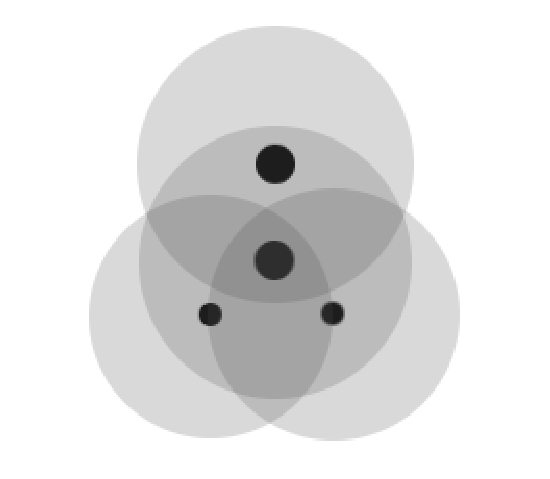
\includegraphics[width=5cm]{03_nevpt/images/rydberg1.eps}
\includegraphics[width=5cm]{03_nevpt/images/rydberg2.eps}
\end{center}
\caption{\footnotesize Two possible schemes to define an augmented basis set
for the description of diffuse Rydberg orbitals: adding diffuse functions on
the single atoms (left side of the picture) or adding diffuse functions
supported by a single dummy atom with no charge. In this thesis, the
development of the Rydberg orbitals followed the second approach.}
\label{fig:rydberg}
\end{figure}
\end{center}


\subsection*{Position of the charge centroid}

The position of the X dummy atom is usually chosen to coincide with the position of
the positive charge centroid, which depends on the molecular geometry and
the excitation performed. Various strategies could be devised in the
evaluation of these coordinates, but practical evaluations performed on
test molecules confirmed the very reduced dependency of the absolute energy
with respect to the dummy atom position. A possible strategy is represented 
by the procedure described by Roos and coworkers\cite{roos-qmescca}.

%A possible strategy is to devise an approximate position by means of the
%dipole $\mu$. For example, in the case of formaldehyde, the higher occupied
%orbitals (by symmetry) for the neutral system are $5a_{1},1b_{1},2b_{2}$.
%The standard geometrical orientation is assumed: the molecule is on the $zy$
%plane, with the carbonyl group along the $z$ axis.  To evaluate the Rydberg
%orbitals for an electronic transition of the type $n_{y} \rightarrow
%\mbox{Ryd}$, an electron is removed from $2b_{2}$. Using the program \dalton
%, a $B_2$ doublet can be evaluated with the following input
%\begin{verbatim}
%**DALTON INPUT
%.RUN WAVE FUNCTION
%.RUN PROPERTIES
%**WAVE FUNCTIONS
%.HF
%*HF INPUT
%.HF OCC
%5 1 1 0
%.MAX DIIS ITERATIONS
%50
%.OPEN SHELL
%3
%**PROPERTIES
%.POPANA
%*END OF INPUT
%\end{verbatim}
%A position for the centroid of the total positive charge can be evaluated
%using the formula
%\beq
%\overrightarrow{R}_{+} = \frac{\sum_{i} e_{+}(i) \overrightarrow{r}_{\! \! +}(i)}{\sum_{i} e_{+}(i)}
%\eeq
%where $i$ runs over the atoms, and $e_{+}(i)$, $\overrightarrow{r}_{\! \! +}(i)$ are
%the nuclear charge and the position of the atom $i$, respectively.
%The same relation could be written for the total negative charge centroid,
%making use of the Mulliken charges
%\beq
%\overrightarrow{R}_{-} = \frac{\sum_{i} e_{-}(i) \overrightarrow{r}_{-}(i)}{\sum_{i} e_{-}(i)}
%\eeq
%but a more accurate value can be obtained using the dipole as provided by \dalton
%\beq
%\overrightarrow{\mu} = \sum_{i} e_{+}(i) \overrightarrow{R}_{+} - \sum_{i} e_{-}(i)
%\overrightarrow{R}_{-}
%\eeq
%Finally, we can obtain the net charge centroid for the ionized molecule
%\beq
%\overrightarrow{R} = \frac{\sum_{i} e_{+}(i) \overrightarrow{R}_{+} + \sum_{i} e_{-}(i)
%\overrightarrow{R}_{-}}{\sum_{i} e_{+}(i) - \sum_{i} e_{-}(i) }
%\eeq
%where the X dummy atom will be placed. 

Another possible strategy is to choose the center of mass. This approach is
simpler, introducing a negligible change in the results, and removes the
need to evaluate the molecular dipole. In the evaluations performed later in
this thesis both approaches have been used, however as already stated
the choice of the position does not produce sizable effects on
the final result.

Once placed, the dummy X atom is provided with an uncontracted basis set.
The exponents for the gaussian functions can be obtained through a
universal algorithm by Kaufmann {\textit et al}\cite{jpb-22-2223-1989}.
\dalton provides an interface to generate these coefficients by means of the
\texttt{.CM FUN} keyword.  The keyword must be provided with three
numbers as defined in Ref. \citen{jpb-22-2223-1989}: the first number
indicates the maximal L quantum number desired for the generated functions.

The second number is related to the starting value for the exponents. The
chosen value gives exponents compatible with small molecules, such as
formaldehyde or acetone.  Kaufmann suggests using a value which provides
exponents in smooth continuity with the core basis set. 

The last number must be equal to or greater than the second, and produces a
new gaussian coefficient for every increment of $\frac{1}{2}$. 

In the performed evaluations the choice (2 2 5.5) has been made.
The first value 2 will generate $s$, $p$ and $d$-type Rydberg diffuse
functions, and the remaining two values 2 and 5.5 produce eight functions.
The final basis set on the X dummy atom is therefore the uncontracted
$8s8p8d$.  Exponents can be extracted from the output file of the \dalton
run.

\subsection*{Contraction of the Rydberg basis set}

The previous section demonstrated how to produce an uncontracted basis set
of diffuse gaussians. These gaussians can be used as-is to enrich the valence
basis set, providing a high number of degrees of freedom in the description of
high-energy Rydberg orbitals, but the resulting basis set is heavily
extended. This introduces a high computational cost and, in the case of
CASPT2 evaluations, convergence problems due to intruder states. 

For these reasons, it is often useful to contract the Rydberg basis set with
appropriate coefficients. A contraction from $8s8p8d$ to $1s1p1d$, for
example, leads to a reduction of the number of additional function from 72
to 9.  A more flexible choice is the contraction to $3s3p3d$, which gives a
good compromise between degrees of freedom and basis set reduction.

An explorative study has been performed to evaluate the influence of Rydberg
contraction on the energy of valence and Rydberg states of formaldehyde.
Tab.~\ref{tbl:rydberg_contraction} reports an evaluation performed on
various excited valence and Rydberg states of the formaldehyde. Details of
the evaluation will be presented in the next section, the only difference
being the basis set, in this case cc-pVTZ\cite{jcp-90-1007-1989}.

As can be seen, the reported values do not change significantly by
decontracting the Rydberg basis set. We can therefore conclude that a
contraction from $8s8p8d$ to $1s1p1d$ is mostly sufficient for obtaining
valuable results.

The procedure to obtain the contraction coefficients has been implemented
\textit{via} both \molcas and \texttt{DALTON}. The \molcas suite provides the \texttt{GENANO}
program, while for the \dalton program an analogous program
\texttt{GENANODAL} has been implemented by our research group.

\begin{center}
\begin{threeparttable}
\footnotesize
\begin{tabular*}{0.70\textwidth}{l@{\hspace{30mm}}cccc}
\hline
                       &  1 Ryd        &  3 Ryd        &  8 Ryd         \\
\hline
                        \multicolumn{4}{c}{\small A$_1$} 	\\
$n_y\!\!\rightarrow\!\! 3p_y$       &   8.14       & 8.14          &  8.14  \\
$n_y\!\!\rightarrow\!\! 3d_{yz}$    &   9.29       & 9.30          &  9.30 \\
$\pi\!\!\rightarrow\!\!\pi^{*}$     &   9.98       & 9.86          &  9.86 \\
                        \multicolumn{4}{c}{\small A$_2$} 	\\
$n_y\!\!\rightarrow\!\!\pi^*$       &   4.05       & 4.03          &  4.04 \\
$n_y\!\!\rightarrow\!\! 3p_x$       &   8.47       & 8.48          &  8.49 \\
$n_y\!\!\rightarrow\!\! 3d_{xz}$    &   9.47       & 9.50          &  9.50 \\
                        \multicolumn{4}{c}{\small B$_2$} 	\\
$n_y\!\!\rightarrow\!\! 3s$               &   7.38       & 7.38          &  7.38 \\
$n_y\!\!\rightarrow\!\! 3p_z$             &   8.29       & 8.24          &  8.24 \\
$n_y\!\!\rightarrow\!\! 3d_{x^2\!-\!y^2}$ &   9.26       & 9.22          &  9.22 \\
$n_y\!\!\rightarrow\!\! 3d_{z^2}$         &   9.43       & 9.39          &  9.39 \\
                        \multicolumn{4}{c}{\small B$_1$} 	\\
$n_y\!\!\rightarrow\!\! 3d_{xy}$          &   9.38       & 9.40          &  9.40 \\
$\sigma\!\!\rightarrow\!\!\pi^{*}$           &   9.37       & 9.33          &  9.33 \\
\hline
\end{tabular*}
\caption{\footnotesize An evaluation of valence and Rydberg excited states transition
energies of formaldehyde, using the cc-pVTZ basis set and different diffuse
basis set contractions. It can be noted that the contraction $8s8p8d$ to
$1s1p1d$ (1 Ryd) produces stable results.\label{tbl:rydberg_contraction}}
\end{threeparttable}
\end{center}


%The theoretical approach is rather simple: a matrix representation of the
%one-particle density matrix must be expressed in the atomic basis set. This
%can be obtained by expressing the one-particle density matrix on a basis set
%of generic spinorbitals $\left\{ \psi_i \left(i\right) \right\}$:
%\beq
%\rho\left(x, x^{\prime}\right) = \sum_{i,j} R_{i,j} \psi_{i} \left( i
%\right) \psi_{j}^{*} \left( x^{\prime} \right)
%\eeq
%Two particular choices of spinorbitals can be defined: the set $\left\{
%\phi_i \left(i\right) \right\}$ of pseudonatural orbitals of a given
%wavefunction and the set of functions used as the atomic basis set $\left\{
%\chi_i \left(i\right) \right\}$. Each one gives the one-particle
%density matrix through a different $R$ matrix
%\beqa
%\rho\left(x, x^{\prime}\right) &=& \sum_{i,j} R^{\mbox{NO}}_{i,j} \phi_{i} \left( i
%\right) \phi_{j}^{*} \left( x^{\prime} \right) \\
%&=& \mathbf{\phi} \mathbf{R}^{NO} \mathbf{\phi} \\
%\rho\left(x, x^{\prime}\right) &=& \sum_{i,j} R^{\mbox{AO}}_{i,j} \chi_{i} \left( i
%\right) \chi_{j}^{*} \left( x^{\prime} \right) \\
%&=& \mathbf{\chi} \mathbf{R}^{AO} \mathbf{\chi} 
%\eeqa
%A matrix of coefficients $\mathbf{C}$ expresses the combination of
%$\mathbf{\chi}$ to obtain $\mathbf{\phi}$
%\beq
%\mathbf{\phi} = \mathbf{\chi} \mathbf{C}
%\eeq
%the $\mathbf{\chi}$ basis set is not orthonormal, since
%\beq
%\mathbf{\chi}^{+}\mathbf{\chi} = \mathbf{S}
%\eeq
%Finally, $\mathbf{R}^{NO}$ is diagonal (given the definition) with
%occupation numbers on the diagonal. In general, the representation
%$R^{\mbox{AO}}$ is not diagonal. The following relation holds:
%\beq
%C^{-1}R^{AO}\left( C^{-1} \right)^{+} = R^{NO}
%\eeq
%Given the following 
%\beq
%\left( C^{-1} \right)^{+} = \left( C^{+} \right)^{-1} = SC
%\eeq
%we obtain
%\beq
%SR^{AO}SC = SCR^{NO}
%\eeq
%Where we obtain the coefficients and eigenvalues of $SR^{AO}S$ in
%a non-unity metric $S$. Once diagonalized, values for the X dummy atom are
%extracted, and a spherical normalization is performed for functions with
%symmetry different from $s$.

\subsection*{Using Molcas}

The procedure using the \molcas suite can be found in the manual
\cite{molcas-site}, and is also reported by Roos et al.\cite{roos-qmescca}.
Here a brief discussion will be presented. The needed steps are:
\begin{itemize}
\item add the diffuse, uncontracted basis set to the molecule (modifying the
\texttt{Seward} input file). The contraction coefficients matrix in this case is a
unit matrix
\item perform a CASSCF evaluation for the system with one electron removed
\item in the resulting output, identify the Rydberg orbitals described by one or
(probably) more functions on the X dummy atom
\item modify the \texttt{.RasOrb} file, containing the orbital coefficients
and their occupation numbers, setting the core occupation numbers to
zero. For the Rydberg orbitals, their occupation numbers must be set
to small, non-zero values, decreasing of one order of magnitude inside each
symmetry. The usual choice is 0.1, 0.01, 0.001 and so on. This prevents
mixing of different Rydberg orbitals inside the same symmetry
\item run the program \texttt{GENANO} with the modified \texttt{RasOrb}
file. This will produce contraction coefficients
\item finally, replace the contraction matrix into the \texttt{Seward} input
file with the new coefficients
\end{itemize}

\subsection*{Using Dalton}

The \dalton suite of programs does not implement a strategy for the
generation of contracted basis sets, therefore an external program has been
developed, named \texttt{GENANODAL}, to accomplish this task. The strategy
is as follows: 
\begin{itemize}
\item perform a Hartree-Fock open shell evaluation for the molecular ion
\item use the program \texttt{IJKLDALI} to perform orbital and integral reordering
\item run the program \texttt{GENANODAL} with an appropriate input, built using the
informations provided by \texttt{IJKLDALI}
\end{itemize}

An example input file is provided:
\begin{verbatim}
&LEGGI FILE11='/scr1/stef/$NAME/FILE11',
       FILE25='/scr1/stef/$NAME/FILE25',
  ZANO=T,NOCCUP=8*0.0,
  0.1,0.01,0.001,0.0001,45*0.0,
  0.0,0.1,0.01,21*0.0,
  0.1,0.01,24*0.0,
  0.1,
  NAOX=72,
  IAOX=23,24,25,26,27,28,29,30,
  64,65,66,67,68,69,70,71,
  92,93,94,95,96,97,98,99,
  31,32,33,34,35,36,37,38,
  39,41,43,45,47,49,51,53,
  40,42,44,46,48,50,52,54,
  72,73,74,75,76,77,78,79,
  100,101,102,103,104,105,106,107,
  111,112,113,114,115,116,117,118,
  MAXL=2,NPRIML=8,8,8,NANOL=1,2,3, &END
\end{verbatim}

\texttt{NOCCUP} have to be set to dummy occupation numbers for each orbital,
honoring the reordering performed by \texttt{IJKLDALI}. As in the case of
\texttt{MOLCAS}, these numbers must be set to values in descending order for the
Rydberg orbitals of the shell we are interested in.

\texttt{NAOX} and \texttt{IAOX} represent how many and which atomic
functions belong to the X dummy atom, repectively. These values must be
extracted from the \texttt{IJKLDALI} output.  The ordering of the functions
must be kept into account: first $s$-type functions, then $p$-type
functions, finally $d$-type functions.

\texttt{MAXL} is the maximal quantum number L to extract. In this case, up to $d$-type
functions are requested.

\texttt{NPRIML} is the number of primitives for each quantum number. For contracting
a $8s8p8d$ Rydberg basis, these values are 8,8,8.

Finally, \texttt{NANOL} are the number of contracted functions generated for each
quantum number L. In this case, provided only as an example, 1 $s$-type
contracted function will be produced, along with 2 $p$-type functions and 3
$d$-type functions. From the output, only the first column of coefficients
will be used.

The \texttt{GENANODAL} code provides exactly the same results as obtained from the
\molcas chain.

%experimental: rydberg della formaldeide e dell'acetone
\section{Evaluation: Rydberg states}

\begin{center}
\textit{This section is based on the article at Ref. \citen{tca-111-352-2004}.}
\end{center}
{\ }\\
\vspace{-1mm}

This section focuses on the description of vertical transitions to valence and
Rydberg excited states with Single-State NEVPT on formaldehyde and acetone.
It aims at completing the detailed description of the excited states of
carbonyl. In the presented evaluation a state-average CASSCF has been
performed. This is different from the previous analysis, where a single state
CASSCF approach was used.

\subsection{Formaldehyde}

The vertical spectrum of the formaldehyde molecule was computed at the
ground state experimental geometry\cite{jms-18-344-1965} (R$_{\mbox{\tiny CO}}$=1.208 \AA,
R$_{\mbox{\tiny CH}}$=1.116 \AA\ and $\theta_{\mbox{\tiny
HCH}}$=116.5$^{\circ}$). As in the previous evaluation, the molecule belongs
to the C$_{2v}$ point group symmetry and lies in the $yz$ plane with the
C and O atoms on the $z$ axis.  The
ANO-1 basis set\cite{tca-77-291-1990} has been used with two different
contraction schemes: the smaller (indicated with ANO(S)) is C,O
[$4s3p1d$]/H[$2s1p$] and the larger (ANO(L)) is C,O
[$6s5p3d2f$]/H[$4s3p2d$].  These valence basis sets have been augmented with
diffuse functions using the procedure described in the previous section, in
order to properly describe the diffuse orbitals involved in the Rydberg
states. These basis functions have been obtained by contraction of a
set of $8s8p8d$ gaussian primitives. Two contraction schemes are considered:
[$1s1p1d$], (Ryd(S)) and [$3s3p3d$], (Ryd(L)).  For a direct comparison
between NEVPT, CASPT2\cite{tca-92-227-1995} and Size-Consistent
Self-Consistent CI ((SC)$^2$-CI)\cite{mp-101-483-2003}, we used in the
calculations the combinations ANO(S)-Ryd(S) and ANO(L)-Ryd(L).

The molecular orbitals are obtained from average CASSCF calculations which
involve the lowest states of a given symmetry. The active spaces, together
with the number and the nature of the states considered in the average
procedure are reported in Tab. \ref{tbl:form_act} and are taken from Ref.
\citen{tca-92-227-1995}.

\input{03_nevpt/tbl_form_act}

The number of orbitals for each irreducible representation
was chosen by the authors so that all the states of interest could be
correctly described. In some cases the active space was enlarged in order
to minimize the effect of the intruder states problem in the CASPT2
calculations.  Given that NEVPT is not affected by the intruder states
problem, in this evaluation a reduction of the active space should be
possible but the comparison of our results with those of Refs.
\citen{tca-92-227-1995} and \citen{mp-101-483-2003} would be in this case less
clear.

The energies of the states are computed in a state specific multireference
perturbation scheme.  The zero-order description of each state is obtained
from a CASCI calculation using the average CASSCF active orbitals. The
inactive orbitals have been canonized to diagonalize the state-specific Fock
matrixes.

A second-order correction to the energy is computed using the NEVPT2 Strongly
Contracted and Partially Contracted variants. All orbitals and
electrons are included in the perturbative treatment. The excitation
energies are computed with respect to the same ground state energy, which is
evaluated as the second order correction to the energy with the reference
energy and wavefunction obtained from a state-specific CASSCF calculation
with four electrons in two $b_1$ ($\pi$ + $\pi^*$) and two $b_2$ ($n_y$ +
virtual) orbitals. This approach for the calculation of the excitation
energies differs from the one used in the CASPT2 calculation, where a
different ground state energy was used for each irreducible representation.

\begin{center}
\begin{threeparttable}
\tiny
\begin{tabular}{lccccccccc}
\hline
Method &2 A$_1$ & 3 A$_1$ & 1 B$_2$ & 2 B$_2$ & 3 B$_2$ & 4 B$_2$ & 2 A$_2$ & 3 A$_2$ &  2 B$_1$ \\
 &($3p_y$) & ($3d_{yz}$) & ($3s$) & ($3p_z$) & 
($3d_{x^2\!-\!y^2}$) & ($3d_{z2}$) & ($3p_x$) &
($3d_{xz}$) & ($3d_{xy}$)     \\
\hline
CASSCF\tnote{a,b}  &   8.07 & 9.18  & 7.37  & 8.15  & 9.08  & 9.21  & 8.84  & 9.78  & 9.16 \\
CASSCF\tnote{a,c}  &   8.04 & 9.12  & 7.29  & 8.08  & 8.99  & 9.12  & 8.81  & 9.72  & 9.12 \\
NEVPT SC\tnote{a,b}&   8.27 & 9.42  & 7.28  & 8.11  & 9.13  & 9.30  & 8.33  & 9.34  & 9.26 \\
                & (0.077)&(0.076)&(0.092)&(0.090)&(0.083)&(0.082)&(0.080)&(0.079)&(0.079)\\
NEVPT SC\tnote{a,c}&   8.39 & 9.56  & 7.32  & 8.16  & 9.17  & 9.37  & 8.46  & 9.48  & 9.39 \\
                & (0.084)&(0.083)&(0.090)&(0.090)&(0.087)&(0.086)&(0.099)&(0.097)&(0.086)\\
NEVPT PC\tnote{a,b}&   8.20 & 9.34  & 7.28  & 8.12  & 9.14  & 9.31  & 8.33  & 9.34  & 9.27 \\
                & (0.084)&(0.084)&(0.095)&(0.093)&(0.085)&(0.084)&(0.082)&(0.081)&(0.081)\\
NEVPT PC\tnote{a,c}&   8.31 & 9.49  & 7.33  & 8.17  & 9.17  & 9.38  & 8.45  & 9.48  & 9.39 \\
                & (0.092)&(0.090)&(0.092)&(0.092)&(0.089)&(0.088)&(0.103)&(0.100)&(0.087)\\
CASPT2 \cite{tca-92-227-1995}
                &   8.12 & 9.24  & 7.30  & 8.09  & 9.13  & 9.31  & 8.32  & 9.31  & 9.23 \\
MC/BMP \cite{cp-205-323-1996}
                &   7.95 & 9.11  & 6.90  & 7.77  & 8.95  & 9.11  & 8.46  & 8.82  & 9.06 \\
(SC)$^2$ CAS+SD\tnote{b} \cite{mp-101-483-2003}
                &   8.14 & 9.26  & 7.17  & 7.96  & 9.00  & 9.19  & 8.30  & 9.28  & 9.12 \\
(SC)$^2$ MR+SD\tnote{c} \cite{mp-101-483-2003}
                &   8.27 & 9.31  & 7.12  & 7.95  & 8.96  & 9.18  & 8.36  & 9.34  & 9.36 \\
CCR(3)$^b$ \cite{mp-101-483-2003}
               &    8.01 & 9.16  & 7.11  & 7.91  & 8.99  & 9.21  & 8.25  & 9.26  & 9.12 \\
CCR(3)$^c$ \cite{mp-101-483-2003}
               &    8.14 & 9.27  & 7.16  & 7.99  & 9.04  & 9.27  & 8.38  & 9.40  & 9.25 \\
MRD-CI \cite{jpc-99-8050-1995}
                &   8.10 & 9.25  & 7.15  & 8.05  & 9.05  & 9.25  & 8.32  & 9.34  & 9.32 \\
MR-CISD + Q \cite{tca-106-369-2001}
                &   8.13 & 9.28  & 7.27  & 8.10  & 9.15  & 9.30  & 8.34  & 9.36  & 9.26 \\
MR-AQCC  \cite{tca-106-369-2001}
                &   8.24 & 9.38  & 7.21  & 8.03  & 9.09  & 9.24  & 8.46  & 9.49  & 9.37 \\
EOM-CCSD \cite{cpl-241-26-1995}
                &   7.99 &10.16  & 6.99  & 7.93  & 9.25  & 9.98  & 8.45  &10.67  & 9.84 \\
EOM-CCSD \cite{jpca-106-4192-2002}
                &   7.98 & 9.13  & 7.04  & 7.88  & 8.94  & 9.12  & 8.21  & 9.29  &10.89 \\
Exp. \cite{robin-hespm}
                &   7.97 &       & 7.11  & 8.14  & 8.88  &       & 8.37  &       &      \\
Exp. \cite{cp-70-291-1982}
                &        &       &       &       &       &       &       &       & 9.22 \\
Exp. \cite{jcsft-281-1643-1985,jcp-85-4228-1986}
                &        &       & 7.09  &       &       &       &       &       &      \\
\hline
\end{tabular}
\caption{\footnotesize Vertical excitation energies (eV) for the Rydberg states of
the formaldehyde molecule.  The numbers in parentheses are the squared norms
of the first order corrections to the wave function. The squared norm for
the ground state is 0.075 (NEVPT SC$^b$), 0.076 (NEVPT PC$^b$), 0.091
(NEVPT SC$^c$) and 0.097 (NEVPT PC$^c$).}
\label{tbl:form_exc_ryd}
\begin{tablenotes}
\footnotesize
\item[a] This work
\item[b] ANO basis set with contraction [$4s3p1d$/$2s1p$] + $1s1p1d$, ANO(S)+Ryd(S)
\item[c] ANO basis set with contraction [$6s5p3d2f$/$4s3p2d$] + $3s3p3d$, ANO(L)+Ryd(L)
\end{tablenotes}
\end{threeparttable}
\end{center}


The vertical excitation energies obtained in our calculations are reported
in Tab. \ref{tbl:form_exc_ryd} for the Rydberg states and in Tab.
\ref{tbl:form_exc_val} for the valence states, together with the previous
theoretical and experimental results.

In Tab. \ref{tbl:form_comparison_1} we show the comparison between our
results and those of Pitarch-Ruiz {\it et al} \cite{mp-101-483-2003}, which
can be considered a good reference since they involve the whole single plus
double excitations space on top of a CAS at a variational level with a
size-consistence correction. We remark that the mean absolute error (MAE) of
our results is always small with the worst case being represented by the
Strongly Contracted NEVPT2 in the ANO(L) + Ryd(L) basis (0.15 eV).  The small
errors appearing in Tab.~\ref{tbl:form_comparison_1} bear out the
reliability of NEVPT2 which can yield results of good accuracy, comparable
with much more refined calculations, but at a reduced computational cost.

For the case of the smaller basis (ANO(S) + Ryd(S)) the CASPT2 results are
also available. NEVPT2 and CASPT2 appear to be of the same quality, with the
former showing in all cases a small squared norm of the wavefunction
perturbation correction thus getting over the intruder states problem.

As to the comparison with the experimental data, beyond a satisfactory
general agreement with our theoretical results we can make the following
observations.

\begin{center}
\begin{threeparttable}
\footnotesize
\begin{tabular*}{0.80\textwidth}{l@{\hspace*{20mm}}ccc}
\hline
Method &4 A$_1$ & 1 A$_2$ & 1 B$_1$ \\
 & (\pipis) & ($n_y\!\!\rightarrow\!\!\pi^*$) & (\sipis) \\
\hline
CASSCF$^{a,b}$          & 10.59  & 5.28  & 9.89  \\
CASSCF$^{a,c}$          & 10.47  & 5.27  & 9.82  \\
NEVPT SC$^{a,b}$        & 10.09  & 4.04  & 9.53  \\
                        & (0.087)&(0.105)&(0.081)\\
NEVPT SC$^{a,c}$        &  9.97  & 3.93  & 9.37  \\
                        & (0.095)&(0.113)&(0.091)\\
NEVPT PC$^{a,b}$        &  9.94  & 4.03  & 9.45  \\
                        & (0.100)&(0.109)&(0.088)\\
NEVPT PC$^{a,c}$        &  9.80  & 3.91  & 9.28  \\
                        & (0.112)&(0.118)&(0.097)\\
CASPT2 \cite{tca-92-227-1995}   &  9.77  & 3.91  & 9.09  \\
MC/BMP \cite{cp-205-323-1996}
                        & 10.37  & 3.83  &13.69  \\ 
(SC)$^2$ CAS+SD$^b$ \cite{mp-101-483-2003}
                        &  9.89  & 4.15  & 9.35  \\
(SC)$^2$ MR+SD$^c$ \cite{mp-101-483-2003}
                        &  9.74  & 4.04  & 9.33  \\
CCR(3)$^b$ \cite{mp-101-483-2003}
                        &  9.80  & 4.01  & 9.29  \\
CCR(3)$^c$ \cite{mp-101-483-2003}
                        &  9.64  & 3.97  & 9.25  \\
MRD-CI \cite{jpc-99-8050-1995}
                        &  9.60  & 4.05  & 9.35  \\
MR-CISD + Q \cite{tca-106-369-2001}
                        &  9.80  & 4.07  & 9.40  \\
MR-AQCC  \cite{tca-106-369-2001}
                        &  9.84  & 4.04  & 9.37  \\
EOM-CCSD \cite{cpl-241-26-1995} &  9.47  & 3.98  & 9.33  \\
EOM-CCSD \cite{jpca-106-4192-2002}&  9.37  & 4.04  & 9.43  \\
Exp. \cite{robin-hespm}      &        & 4.07  &       \\
Exp. \cite{jcp-87-3796-1987}      &        & 3.79  &       \\
\hline
\end{tabular*}
\caption{\footnotesize Vertical excitation energies (eV) for the valence states of
the formaldehyde molecule.  The numbers in parentheses are the squared norms
of the first order corrections to the wavefunction. The squared norm for
the ground state is 0.075 (NEVPT SC$^b$), 0.076 (NEVPT PC$^b$), 0.091
(NEVPT SC$^c$) and 0.097 (NEVPT PC$^c$).}
\label{tbl:form_exc_val}
\begin{tablenotes}
\footnotesize
\item[a] This work
\item[b] ANO(S)+Ryd(S) basis (see text)
\item[c] ANO(L)+Ryd(L) basis (see text)
\end{tablenotes}
\end{threeparttable}
\end{center}


First, in accordance with most theoretical calculations our vertical
2~$^1$A$_1$  and 1~$^1$B$_2$ Rydberg transitions appear in inverted order
with respect to experimental adiabatic transitions \cite{robin-hespm}: a
more stringent comparison would require the calculation of adiabatic
transition with due allowance for the zero point energy correction

Second, the calculation of the $^1$A$_1$ Rydberg states with the larger basis
set introduces one more Rydberg state ($n_y\rightarrow\pi^*$) below the
valence $\pi\rightarrow\pi^*$. Such state has been ignored in the average
CASSCF since we were interested in transitions involving Rydberg orbitals
not exceeding the quantum number $n=3$

Finally, mixing between Rydberg and valence character may occur in both the
$^1$A$_1$ and $^1$B$_1$ transitions \cite{tca-92-227-1995,jpc-99-8050-1995}.
For a correct treatment of such states a quasi-degenerate treatment
is required \cite{acp-67-1-1987,cpl-288-299-1998}.

\begin{center}
\begin{threeparttable}
\footnotesize
\begin{tabular*}{0.80\textwidth}{l@{\hspace*{15mm}}ccc}
\hline
         & NEVPT PC\tnote{a}& NEVPT SC\tnote{a} & CASPT2\tnote{b}    \\
\hline
2 A$_1$  & $~$0.06 & $~$0.13  &    -0.02  \\
3 A$_1$  & $~$0.08 & $~$0.16  &    -0.02  \\
4 A$_1$  & $~$0.05 & $~$0.20  &    -0.12  \\
1 B$_2$  & $~$0.11 & $~$0.11  &  $~$0.13  \\
2 B$_2$  & $~$0.16 & $~$0.15  &  $~$0.13  \\
3 B$_2$  & $~$0.14 & $~$0.13  &  $~$0.13  \\
4 B$_2$  & $~$0.12 & $~$0.11  &  $~$0.12  \\
1 A$_2$  &   -0.12 &   -0.11  &    -0.24  \\
2 A$_2$  & $~$0.03 & $~$0.03  &  $~$0.02  \\
3 A$_2$  & $~$0.06 & $~$0.06  &  $~$0.03  \\
1 B$_1$  & $~$0.10 & $~$0.18  &    -0.26  \\
2 B$_1$  & $~$0.15 & $~$0.14  &  $~$0.11  \\
\hline
MAE\tnote{c}   & $~$0.10 & $~$0.13  &  $~$0.11  \\
\hline
\end{tabular*}
\caption{\footnotesize 
Energy differences (eV) between the perturbation and the (SC)$^2$ CAS+SD
results of Ref. \citen{mp-101-483-2003}
}
\label{tbl:form_comparison_1}
\begin{tablenotes}
\footnotesize
\item[a] This work
\item[b] Ref. \citen{tca-92-227-1995}
\item[c] Mean Absolute Error
\end{tablenotes}
\end{threeparttable}
\end{center}





\subsection{Acetone}

The computational strategy used for acetone closely follows the one applied
to formaldehyde. The vertical spectrum has been computed at the ground
state experimental geometry \cite{jms-18-344-1965}. The molecule belongs to
the C$_{2v}$ point group symmetry with the OCCC skeleton in the $yz$
plane (C and O atoms on the $z$ axis and with an orientation of the CH$_3$ 
groups that place the two H atoms lying in the $yz$ plane as far as
possible). For acetone, we only consider the C,O[$4s3p1d$]/H[$2s1p$]
contraction of the ANO basis set. The Rydberg states are described using a
set of $8s8p8d$ diffuse functions contracted to $1s1p1d$. 

As in formaldehyde, average CASSCF calculations provide the molecular
orbitals: the active spaces and the number and the nature of the states
considered in the average procedure are reported in Tab. \ref{tbl:aceto_act}
and are taken from Ref. \citen{jcp-104-1791-1996}. 

With respect to formaldehyde, the active space has been modified adding the
two CO $\sigma$ and $\sigma^*$ orbitals and the two CO $\sigma$ electrons,
except for the A$_1$ symmetry where three virtual orbitals (one of $b_1$ and
two of $b_2$ symmetry) have been removed. In Ref. \citen{jcp-104-1791-1996}
the CO $\sigma$ and $\sigma^*$ orbitals have been added to the active space
to correctly describe the adiabatic electronic transitions for the
valence states, in which an elongation of the CO bond is observed.
% due to the
% promotion of an electron to the $\pi^{*}$ orbital.

Given that we present here only results on the vertical transitions, also in
the case of acetone a reduction of the active space used in Ref.
\citen{jcp-104-1791-1996} would have been possible, but we have chosen to
maintain the same active space in order to have a meaningful comparison with
the CASPT2 data.

\begin{center}
\begin{threeparttable}
\begin{tabular*}{0.80\textwidth}{clc}
\hline\noalign{\smallskip}
\# MOs \tnote{a} & Symmetry and nature of states    & \# states\tnote{b} \\
\noalign{\smallskip}\hline\noalign{\smallskip}
    (2230)   & $^1$A$_1$ (GS; $n_y\!\rightarrow\! 3p_y$,$3d_{yz}$; $\pi\!\rightarrow\!\pi^*$) & 4 \\
    (2200)   & $^1$B$_1$ ($\sigma\!\rightarrow\!\pi^*$) & 1\\
    (2211)   & $^1$B$_1$ ($n_y\!\rightarrow\! 3d_{xy}$) & 1 \\
    (6210)   & $^1$B$_2$ ($n_y\!\rightarrow\! 3s$, $3p_z$, $3d_{x^2\!-\!y^2}$, $3d_{z^2}$) & 4 \\
    (2410)   & $^1$A$_2$ ($n_y\!\rightarrow\!\pi^*$, $3p_x$, $3d_{xz}$) & 3 \\
\noalign{\smallskip}\hline
\end{tabular*}
\caption{\footnotesize Active spaces and number of states used in the average CASSCF
calculations for the acetone molecule (always 6 active electrons except in
the case of the $^1$B$_1$ ($\sigma\rightarrow\pi^*$) which is computed with
4 active electrons)}
\label{tbl:aceto_act}
\begin{tablenotes}
\footnotesize
\item[a] number of molecular orbitals in the active space for the four
irreducible representations ($a_1$,$b_1$,$b_2$,$a_2$)
\item[b] number of states used in the average procedure
\end{tablenotes}
\end{threeparttable}
\end{center}


The energies of the states are computed following the strategy outlined for
formaldehyde and the transition energies are reported in Tab.
\ref{tbl:aceto_exc_ryd} for the Rydberg states and in Tab.
\ref{tbl:aceto_exc_val} for the valence states, together with the results of
other theoretical calculations and with some experimental results.

We note that our Partially Contracted NEVPT2 results compare very well with
the CASPT2 ones.  We also remark that in two of the valence transitions
(4~$^1$A$_1$, $\pi\rightarrow\pi^*$ and 1~$^1$A$_2$, $n_y\rightarrow\pi^*$)
the difference between Strongly and Partially Contracted NEVPT2 appears to be
unusually sizable (0.59 eV and 0.20 eV, respectively). We think that this is
symptom for the zero-order wavefunction to necessitate significant
improvement.

\begin{center}
\begin{threeparttable}
\tiny
\begin{tabular}{lccccccccc}
\hline
Method &2 A$_1$ & 3 A$_1$ & 1 B$_2$ & 2 B$_2$ & 3 B$_2$ & 4 B$_2$ & 2 A$_2$ & 3 A$_2$ &  2 B$_1$ \\
 &($3p_y$) & ($3d_{yz}$) & ($3s$) & ($3p_z$) & 
($3d_{x^2\!-\!y^2}$) & ($3d_{z2}$) & ($3p_x$) &
($3d_{xz}$) & ($3d_{xy}$)     \\
\hline
CASSCF\tnote{a}  &  7.91  & 8.46  & 6.02  & 6.75  & 7.30  & 7.39  & 7.29  & 7.99  & 7.38  \\
NEVPT2 SC\tnote{a}&  7.40  & 8.03  & 6.75  & 7.67  & 8.25  & 8.37  & 7.48  & 8.24  & 8.36  \\
            & (0.182)&(0.179)&(0.159)&(0.155)&(0.154)&(0.153)&(0.168)&(0.166)&(0.154)\\
NEVPT2 PC\tnote{a}&  7.27  & 7.91  & 6.71  & 7.64  & 8.22  & 8.34  & 7.39  & 8.17  & 8.35  \\
            & (0.195)&(0.192)&(0.166)&(0.161)&(0.160)&(0.158)&(0.177)&(0.175)&(0.158)\\
CASPT2 \cite{jcp-104-1791-1996}
            &  7.26  & 7.91  & 6.58 & 7.48   & 8.04  & 8.18  & 7.34  & 8.09  & 8.20  \\
EOM-CCSD \cite{cpl-241-26-1995}
            &  7.45  & 8.23  & 6.39 & 7.51   & 7.95  & 8.48  & 7.41  & 8.44  & 8.43  \\
EOM-CCSD \cite{jpca-106-4192-2002}
            &  7.41  & 8.02  & 6.42 & 7.39   & 7.82  & 8.10  & 7.31  & 8.04  & 8.11  \\
Exp.\cite{jcp-104-1791-1996}
            &        & 7.8   &      &        & 8.09  &       &       &       & 8.17  \\
Exp.\cite{jcp-98-3795-1993}
            &        &       & 6.35 &        &       &       &       &       &       \\
Exp.\cite{robin-hespm}
            &        &       & 6.36 &        &       &       & 7.45  &       &       \\
Exp.\cite{jcp-89-6086-1988}
            &  7.41  &       &      & 7.45   &       &       & 7.36  &       &       \\
\hline
\end{tabular}
\caption{\footnotesize Vertical excitation energies (eV) for the Rydberg states of
the acetone molecule}
\label{tbl:aceto_exc_ryd}
\begin{tablenotes}
\footnotesize
\item[a] This work. The numbers in parentheses are the squared norms of the
first order corrections to the wavefunction. The squared norm for the
ground state is 0.164 (NEVPT2 SC) and 0.167 (NEVPT2 PC).
\end{tablenotes}
\end{threeparttable}
\end{center}


\begin{center}
\begin{threeparttable}
\footnotesize
\begin{tabular*}{0.80\textwidth}{l@{\hspace*{20mm}}ccc}
\hline
Method &4 A$_1$ & 1 A$_2$ & 1 B$_1$ \\
 & (\pipis) & ($n_y\!\!\rightarrow\!\!\pi^*$) & (\sipis) \\
\noalign{\smallskip}\hline\noalign{\smallskip}
CASSCF\tnote{a}             & 11.60  & 5.57  &10.38 \\
NEVPT2 SC\tnote{a}           &  9.60  & 4.42  & 9.29 \\
                       & (0.204)&(0.189)&(0.182)\\
NEVPT2 PC\tnote{a}           &  9.01  & 4.22  & 9.23 \\
                       & (0.293)&(0.207)&(0.190)\\
CASPT2 \cite{jcp-104-1791-1996}  &  9.16  & 4.18  & 9.10 \\
EOM-CC \cite{cpl-241-26-1995}  &  9.15  & 4.48  & 9.30 \\
EOM-CC \cite{jpca-106-4192-2002} &  8.52  & 4.47  & 8.87 \\
Exp. \cite{jcp-87-3796-1987}     &        & 4.38  &      \\
Exp. \cite{robin-hespm}     &        & 4.43  &      \\
\hline
\end{tabular*}
\caption{\footnotesize Vertical excitation energies (eV) for the valence states of
the acetone molecule}
\label{tbl:aceto_exc_val}
\begin{tablenotes}
\footnotesize
\item[a] This work.  The numbers in parentheses are the squared norms of the
first-order corrections to the wavefunction. The squared norm for the
ground state is 0.164 (NEVPT2 SC) and 0.167 (NEVPT2 PC).
\end{tablenotes}
\end{threeparttable}
\end{center}



\subsection*{Final remarks}

Among the formal requirements satisfied by NEVPT2, the absence of intruder
states appears particularly interesting for the application to the
calculation of electronically excited states. The results shown in the
precedent section for the vertical transitions of formaldehyde and acetone
are of good quality and exhibit good agreements with the best calculations so
far performed as well as with the existing experimental data. 

Our calculations have been carried out starting from rather modest size
CASSCF wavefunctions. The computational overhead involved by the two forms
of NEVPT2 (Strongly and Partially Contracted) amounts to only a small
fraction of the CASSCF calculation for such small active orbital spaces and
this favorable situation is not expected to drastically change when passing
on to larger molecules, provided that the active space can be kept within
manageable dimensions.

No evidence of divergences or misbehaviors in the perturbation summation
has been found in the calculation of the Rydberg states, which are
particularly prone to exhibiting the appearance of intruder states. 

%estensione all'analisi caso qd
\section{Quasi-Degenerate NEVPT2}

Single-State NEVPT2, presented in the previous sections, performs the
perturbative treatment on a given state, disregarding possible interaction
between multiple states which are nearly degenerate before or after the
perturbation. This is due to the definition of a state-specific zero-order
Hamiltonian. To address the needs for quasi-degeneracy problems, frequently
encountered when analyzing avoided crossings, the Quasi-Degenerate NEVPT2
(QD-NEVPT) approach has been implemented\cite{jcp-121-4043-2004}. 

The approach used for NEVPT follows the description made by
Lindgren\cite{jpb-7-2441-1974}.  We define a model space, as generated by a
set of $n$ eigenfunctions, in our case of CASSCF type $\left\{ \Psi_1^{(0)},
\Psi_2^{(0)},\ldots, \Psi_n^{(0)} \right\}$ which undergo altogether the
perturbative correction.  These functions define a space $\mathcal{P}$, and
have associated zero-order energies $E_i^{(0)}$.  We can also define the
complementary space $\mathcal{Q} = 1 - \mathcal{P}$ with
the set of functions $\left\{ \Psi_{n+1}^{(0)}, \Psi_{n+2}^{(0)}, \ldots
\right\}$. Projection operators can be defined for each space
\beqa
\hat{\mathcal{P}} &=& \sum_{i=1}^{n} \ket{\Psi_{i}^{(0)}} \bra{\Psi_{i}^{(0)}} \\
\hat{\mathcal{Q}} &=& \sum_{a > n} \ket{\Psi_{a}^{(0)}} \bra{\Psi_{a}^{(0)}} 
\eeqa
It can be demonstrated that the following relationships hold
\beqa
\label{eqn:qdpt_4}
\hat{\mathcal{P}}^2 = \hat{\mathcal{P}}^{+} = \hat{\mathcal{P}} \\
\hat{\mathcal{P}} \hat{\mathcal{Q}} = \hat{\mathcal{Q}} \hat{\mathcal{P}} = 0 
\eeqa
%\commut{\hat{\mathcal{P}}}{\ham_0} = \commut{\hat{\mathcal{Q}}}{\ham_0} = 0
Defining the true eigenfunctions of the Schr\"odinger equation as
\beq
\ham \Psi_i = E_i \Psi_i
\eeq
we can now write the projection of the true eigenfunctions inside the
spaces defined above
\beqa
\tilde{\Psi}_i &=& \hat{\mathcal{P}} \Psi_i \qquad \forall 1 \le i \le n \\ 
\tilde{\Psi}_a &=& \hat{\mathcal{Q}} \Psi_a \qquad \forall a > n 
\eeqa
and define a ``wave operator'' $\hat{\Omega}$ which produces the true
eigenfunctions $\Psi_i$ from the projected ones
\beq
\hat{\Omega}\tilde{\Psi}_i = \Psi_i 
\eeq
but produces zero when applied to the complementary space
\beq
\hat{\Omega}\tilde{\Psi}_a = 0
\eeq
It can be proved that the following relationships hold
\beqa
\hat{\mathcal{P}} \hat{\Omega} &=& \hat{\mathcal{P}} \\
\hat{\Omega} \hat{\mathcal{P}} &=& \hat{\Omega} \\
\hat{\Omega} \hat{\mathcal{Q}} &=& 0
\eeqa
It is possible to rewrite the Schr\"odinger equation in the form
\beq
\label{eqn:qdpt_2}
\ham \hat{\Omega} \tilde{\Psi}_i = E_i \hat{\Omega} \tilde{\Psi}_i
\eeq
and applying $\hat{\mathcal{P}}$ on both sides
\beqa
\hat{\mathcal{P}} \ham \hat{\Omega} \tilde{\Psi}_i &=& E_i \tilde{\Psi}_i \\
\label{eqn:qdpt_1}
\ham_{\mbox{\tiny eff}} \tilde{\Psi}_i &=& E_i \tilde{\Psi}_i
\eeqa
where an effective Hamiltonian $\ham_{\mbox{\tiny eff}} = \hat{\mathcal{P}} \ham
\hat{\Omega}$ has been defined.  This Hamiltonian produces the eigenvalues
$E_i$ of the true Hamiltonian, but operates in the model space.


The final goal of this technique is to obtain the matrix
$\braket{\Psi_n^{(0)}}{\ham_{\mbox{\tiny eff}}}{\Psi_m^{(0)}}$ and diagonalize it.
This matrix has the dimensionality of the number of states considered in the
Quasi-Degenerate scheme. Once diagonalized, it provides the corrected
energies and the coefficients mixing the perturbed wavefunctions.

To accomplish this task, further elaborations are needed: making use of
Eqn.~\ref{eqn:qdpt_1} by applying on both sides
$\hat{\Omega}$ and subtracting \ref{eqn:qdpt_2} we obtain
\beq
\left( \hat{\Omega} \ham_{\mbox{\tiny eff}} - \ham \hat{\Omega} \right)
\tilde{\Psi}_i = 0
\eeq
which is valid also for $\tilde{\Psi}_a$, therefore the operator itself is
zero
\beq
\hat{\Omega} \ham_{\mbox{\tiny eff}} - \ham \hat{\Omega} = 0
\eeq
Replacing the definition of $\ham_{\mbox{eff}}$ we obtain the
generalized Bloch equation
\beq
\hat{\Omega} \hat{\mathcal{P}} \ham \hat{\Omega} - \ham \hat{\Omega} = 0
\eeq

Introducing the expression of the Hamiltonian as $\ham = \ham_0 + \hat{V}$
we can now perform a substitution inside the Bloch equation to obtain 
\beq
\commut{\hat{\Omega}}{\ham_0} = \hat{\mathcal{Q}} \hat{V} \hat{\Omega} -
\hat{\mathcal{Q}} \hat{\Omega} \hat{\mathcal{P}} \hat{V} \hat{\Omega}
\eeq
To proceed further in the development, a perturbative expansion for the wave
operator and the effective Hamiltonian is performed
\beq
\hat{\Omega} = \hat{\mathcal{P}} + \hat{\Omega}^{(1)} + \hat{\Omega}^{(2)} + \dots
\eeq
and the following relationships can be obtained
\beqa
\commut{\hat{\Omega}^{(1)}}{\ham_0} &=& \hat{\mathcal{Q}} \hat{V}
\hat{\mathcal{P}} \label{eqn:qdpt_6}\\
\commut{\hat{\Omega}^{(2)}}{\ham_0} &=& \hat{\mathcal{Q}} \hat{V}
\hat{\Omega}^{(1)} - \hat{\mathcal{Q}} \hat{\Omega}^{(1)} \hat{\mathcal{P}}
\hat{V} \hat{\mathcal{P}} \\
&\vdots& \nonumber
\eeqa 

Applying the commutator in \ref{eqn:qdpt_6} to $\ket{\Psi_i}$ and
keeping into account that $\hat{\mathcal{Q}} \hat{\Omega}^{(1)} =
\hat{\Omega}^{(1)}$ we obtain
\beq
\left( E_i^{(0)} - \hat{\mathcal{Q}} \ham_0 \hat{\mathcal{Q}} \right)
\hat{\Omega}^{(1)} \ket{\Psi_i} = \hat{\mathcal{Q}} \hat{V} \ket{\Psi_i}
\eeq
which can be rearranged to produce
\beq
\hat{\Omega}^{(1)} \ket{\Psi_i^{(0)}} = \left( E_i^{(0)} - \hat{\mathcal{Q}}
\ham_0 \hat{\mathcal{Q}} \right)^{-1} \hat{\mathcal{Q}} \hat{V}
\ket{\Psi_i^{(0)}}
\eeq
and knowing that
\beq
\hat{\mathcal{Q}} \ham_0 \hat{\mathcal{Q}} = \sum_{a} \ket{\Psi_a^{(0)}}
E_a^{(0)} \bra{\Psi_a^{(0)}}
\eeq
we obtain
\beq
\hat{\Omega}^{(1)} \ket{\Psi_i^{(0)}} = \sum_{a > n} \ket{\Psi_a^{(0)}}
\frac{\braket{\Psi_a^{(0)}}{\hat{V}}{\Psi_i^{(0)}}}{E_i^{(0)} - E_a^{(0)}}
\eeq

We can now apply the perturbative expansion also to $\ham_{\mbox{\tiny eff}}$
\beq
\ham_{\mbox{\tiny eff}} =  \ham_{\mbox{\tiny eff}}^{(0)} + \ham_{\mbox{\tiny
eff}}^{(1)} + \ham_{\mbox{\tiny eff}}^{(2)} + \dots
\eeq
to obtain the following terms
\beqa
\ham_{\mbox{\tiny eff}}^{(0)} &=& \hat{\mathcal{P}} \ham^{(0)} \hat{\mathcal{P}} \\
\ham_{\mbox{\tiny eff}}^{(1)} &=& \hat{\mathcal{P}} \hat{V} \hat{\mathcal{P}} = 0 \\
\ham_{\mbox{\tiny eff}}^{(2)} &=& \hat{\mathcal{P}} \hat{V} \hat{\Omega}^{(1)}  \\
&\vdots&
\eeqa
hence, the $\mathbf{H}_{\mbox{\tiny eff}}$ matrix up to the second-order
can be obtained from the formulation of the $\ham_{\mbox{\tiny eff}}^{(2)}$ operator. 

When applying the above formulations to the NEVPT case, we have to consider
that the model space is generated by the CAS wavefunctions $\left\{
\Psi_m^{(0)} \right\}$, and the zero-order Hamiltonian is defined through its
spectral decomposition
\beqa
\ham_0(m) &=& \ket{\Psi_m^{(0)}} E_m^{(0)} \bra{\Psi_m^{(0)}} \\
&&+ \sum_{m^{\prime} \neq m} \ket{\Psi_{m^{\prime}}^{(0)}} E_{m^{\prime}}^{(0)}
\bra{\Psi_{m^{\prime}}^{(0)}} \\
&&+ \sum_{l,k,\mu} \ket{\Psi_{l,\mu}^{k}(m)} E_{l,\mu}^{k}(m)
\bra{\Psi_{l,\mu}^{k}(m)}
\eeqa
where $\Psi_{l,\mu}^{k}(m)$ are the perturbers generated by the
application of excitation operators to the state $m$. As a consequence, the
zero-order Hamiltonian is state dependen. A partition of the Hamiltonian in
a state-specific way is needed using the multipartitioning
approach\cite{cpl-233-597-1995}. For each state $m$ we define a different
partitioning scheme of the Hamiltonian
\beq
\ham = \ham_0(m) + \hat{V}(m) 
\eeq
It must be noted however that both spaces $\mathcal{P}$ and $\mathcal{Q}$
(and consequently the projection operators) are not state-specific, since
$\mathcal{P}$ is defined by the CAS space, and $\mathcal{Q} = 1 -
\mathcal{P}$. We obtain for $\hat{\Omega}^{(1)}$
\beq
\hat{\Omega}^{(1)} \ket{\Psi_m^{(0)}} = \sum_{k,l,\mu}
\frac{\ket{\Psi_{l,\mu}^{k}(m)}
\braket{\Psi_{l,\mu}^{k}(m)}{\ham}{\Psi_{m}^{(0)}}}{E_m^{(0)} -
E_{l,\mu}^{k}(m)}
\eeq
and the final $\ham_{\mbox{\tiny eff}}$ matrix element is therefore
\beq
\braket{\Psi_n^{(0)}}{\ham_{\mbox{\tiny eff}}}{\Psi_m^{(0)}} = \delta_{nm}
E_m^{(0)} + \sum_{l,k,\mu}
\frac{\braket{\Psi_n^{(0)}}{\ham}{\Psi_{l,\mu}^{k}(m)}
\braket{\Psi_{l,\mu}^{k}(m)}{\ham}{\Psi_m^{(0)}}}{E_m^{(0)} -
E_{l,\mu}^{k}(m)}
\eeq

It can be noted that the diagonal elements of the obtained matrix are the
single state contributions. In a Single-State approach, the non-diagonal
elements of the effective matrix are assumed as zero. The Quasi-Degenerate
approach provides these non-diagonal elements, whose role is to mix the
perturbed wavefunctions.

The $\mathbf{H}_{\mbox{\tiny eff}}$ matrix in general is not hermitian, but a
hermitian variant can be obtained\cite{np-20-321-1960}:
\beq
\mathbf{H}_{\mbox{\tiny eff}}^{\prime} = \mathbf{S}^{-\frac{1}{2}}
\mathbf{H}_{\mbox{\tiny eff}} \mathbf{S}^{\frac{1}{2}}
\eeq
with $S_{ij} = \integral{\tilde{\Psi}_i}{\tilde{\Psi}_j}$.


%procedura sperimentale qdpt
\section{Evaluation: QDPT on formaldehyde}

\begin{center}
\textit{This section is based on the article at Ref. \citen{ijqc-2005}} \\
\end{center}
{\ }\\
\vspace{-5mm}

A Quasi-Degenerate NEVPT2 evaluation has been conducted over the
formaldehyde molecule. Four electronic states of A$_1$ symmetry have been
considered in the analysis, namely the ground state (1A$_1$), the $n_y \rightarrow
3p_y$ Rydberg state (2A$_1$), the $n_y \rightarrow 3d_{yz}$ Rydberg state
(3A$_1$) and the $\pi \rightarrow \pi^{*}$ valence state (4A$_1$). 

The energy curves for these states have been studied as a function of the CO
distance. The rationale behind this study is to analyze the qualitative
behavior of the avoided crossing of the potential energy curves arising from
these states.  A simple CASSCF wavefunction does not keep fully into account
the dynamic correlation needed for the description of the ground and $\pi
\rightarrow \pi^{*}$ state. These states require higher correlative
corrections than the ones needed by the Rydberg states, due to the high
average distance of the promoted electron from the molecular framework in
the Rydberg case.  Also, the large mixing occurring between Rydberg and
valence states invokes the need for a Quasi-Degenerate treatment.

A state averaged CASSCF procedure with an active space of six electrons in
seven orbitals has been performed. The interested active orbitals are the
$\sigma$, $\sigma^{*}$, the $\pi$, $\pi^{*}$, the $n_y$ and the $3p_y$ and
$3d_{yz}$ Rydberg orbitals. To describe the potential curve, CO bond
distances from 2.00 bohr to 3.40 bohr have been considered, with a step of
0.1 bohr.  Occasionally, the step length has been reduced to address
particular features of the curves. Other geometrical parameters have been
kept fixed at the values obtained by a HF/MP2 complete optimization with
the same basis set.

The basis set is the ANO-1, augmented with a Rydberg set of functions built
as detailed in Sec. \ref{sec:rydberg_procedure}. The contraction scheme
produced a set [$1s1p1d$] from a decontracted set of diffuse functions
[$8s8p8d$], centered on the charge centroid evaluated at the ground state
geometry. The position of the centroid is unchanged during the CO
elongation, given its marginal influence on the final results.

The procedure is briefly presented here: for each molecular geometry an
averaged CASSCF evaluation has been performed, producing a set of averaged
molecular orbitals. For each state, the average orbitals are brought in
canonical form in the inactive set. 

\begin{center}
\begin{figure}[ht]
\begin{center}
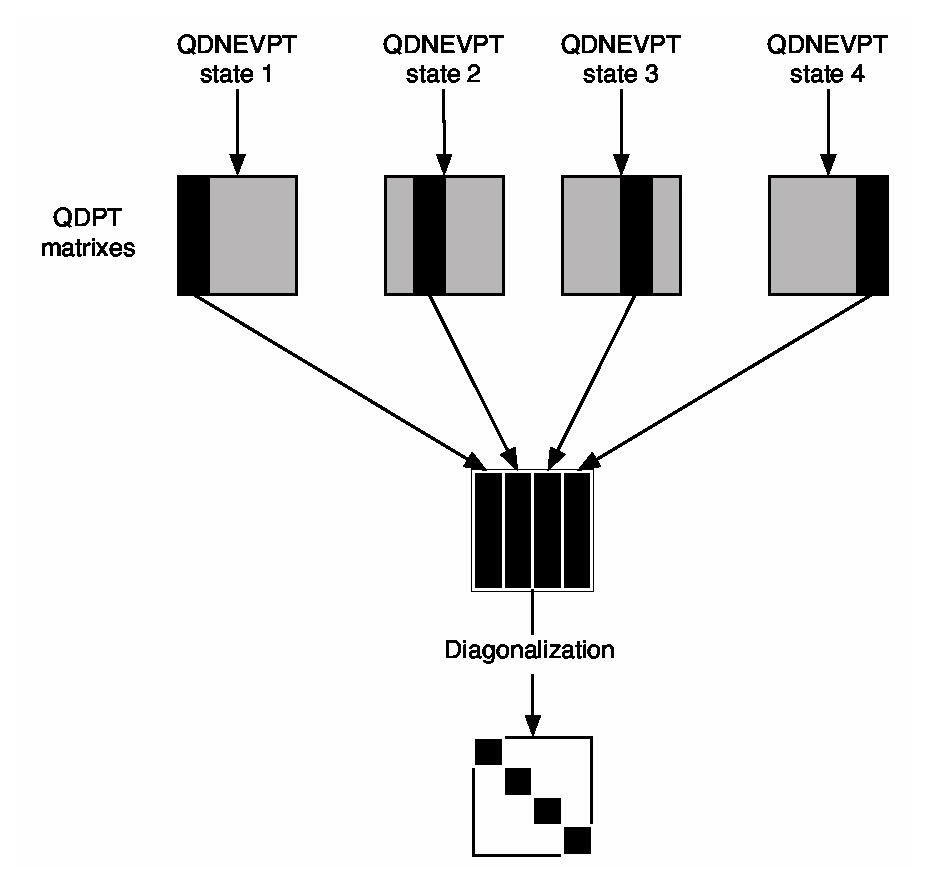
\includegraphics[width=10cm]{03_nevpt/images/qdpt_diagram-gimped.eps}
\end{center}
\caption{\footnotesize The computational scheme for the evaluation of the
Quasi Degenerate treatment. Four different QDPT matrixes are obtained by the
procedure, each one referring to a particular state. A single column is
extracted from each matrix and gathered in a final matrix which is
diagonalized. }
\label{fig:qdpt_diagram}
\end{figure}
\end{center}


This procedure provides four orbital sets, which are used in the Quasi-Degenerate evaluation. Four matrixes are obtained (refer to Fig.
\ref{fig:qdpt_diagram}) each one referring to a particular state. To build
the final effective Hamiltonian matrix to be diagonalized, the following
steps must be applied:
\begin{enumerate}
\item decompose the four matrixes columnwise
\item extract the column number $n$ from the matrix referring to the $n$-th
electronic state
%\item check if coupling (non-diagonal) elements have the correct sign
\item build a final matrix, made of the obtained columns
\item diagonalize it to obtain the final energies and coefficients
\end{enumerate}

%Some explanation have to be reported for the third point: non-diagonal
%elements refer to integrals
%$\braket{\Psi_n^{(0)}}{\ham_{\mbox{eff}}}{\Psi_m^{(0)}}$. The computational
%procedure followed by each matrix is the same, but the final wavefunctions
%can differ in sign. As an example, in the evaluation of the first state the
%element $\braket{\Psi_2^{(0)}}{\ham_{\mbox{eff}}}{\Psi_1^{(0)}}$ can be
%referred to wavefunction with the same sign. For the evaluation of
%$\braket{\Psi_1^{(0)}}{\ham_{\mbox{eff}}}{\Psi_2^{(0)}}$, the sign of
%$\Psi_2^{(0)}$ can be different. A direct comparison of the two integrals is
%not possible, due to their different absolute values.

%A possible solution is to choose as a reference the evaluation matrix provided
%by the first electronic state.  Orbitals for the remaining states are
%preserved only in the inactive part, while the active part is replaced with
%the orbitals from the first set. This approach is formally correct since the
%CAS evaluation is a Full-CI inside this orbital space, and the NEVPT
%treatment is invariant for orbital mixing inside the active block. A quick
%check for the sign of the CI coefficients now can be performed, an
%appropriate sign adaptation for each element of the final matrix. The
%procedure has been implemented as an automatic bash script to prevent
%errors from a manual process.

The curves obtained at CASSCF level are represented in Fig.
\ref{fig:formaldehyde_cas_curve}. The main feature is the behavior of the
$\pi \rightarrow \pi^{*}$ 4A$_1$ state with respect to 2A$_1$ and 3A$_1$
Rydberg states. The Rydberg states are nearly parallel to the ground state.
This is expected since the electron is promoted from a non-bonding orbital
to a distant one, introducing very little destabilization in the electronic
asset that governs the molecular geometry.

On the other hand, the valence
excited state introduces a serious variation in this asset, moving from a
double bond situation to a nearly single bond situation. This imposes a
steep elongation of the bond, and the potential energy curve for this state
crosses the Rydberg ones. Due to interaction between these states, an
avoided crossing situation occurs, producing the resulting diagram.
\vspace{-3mm}
\begin{center}
\begin{figure}[ht]
\begin{center}
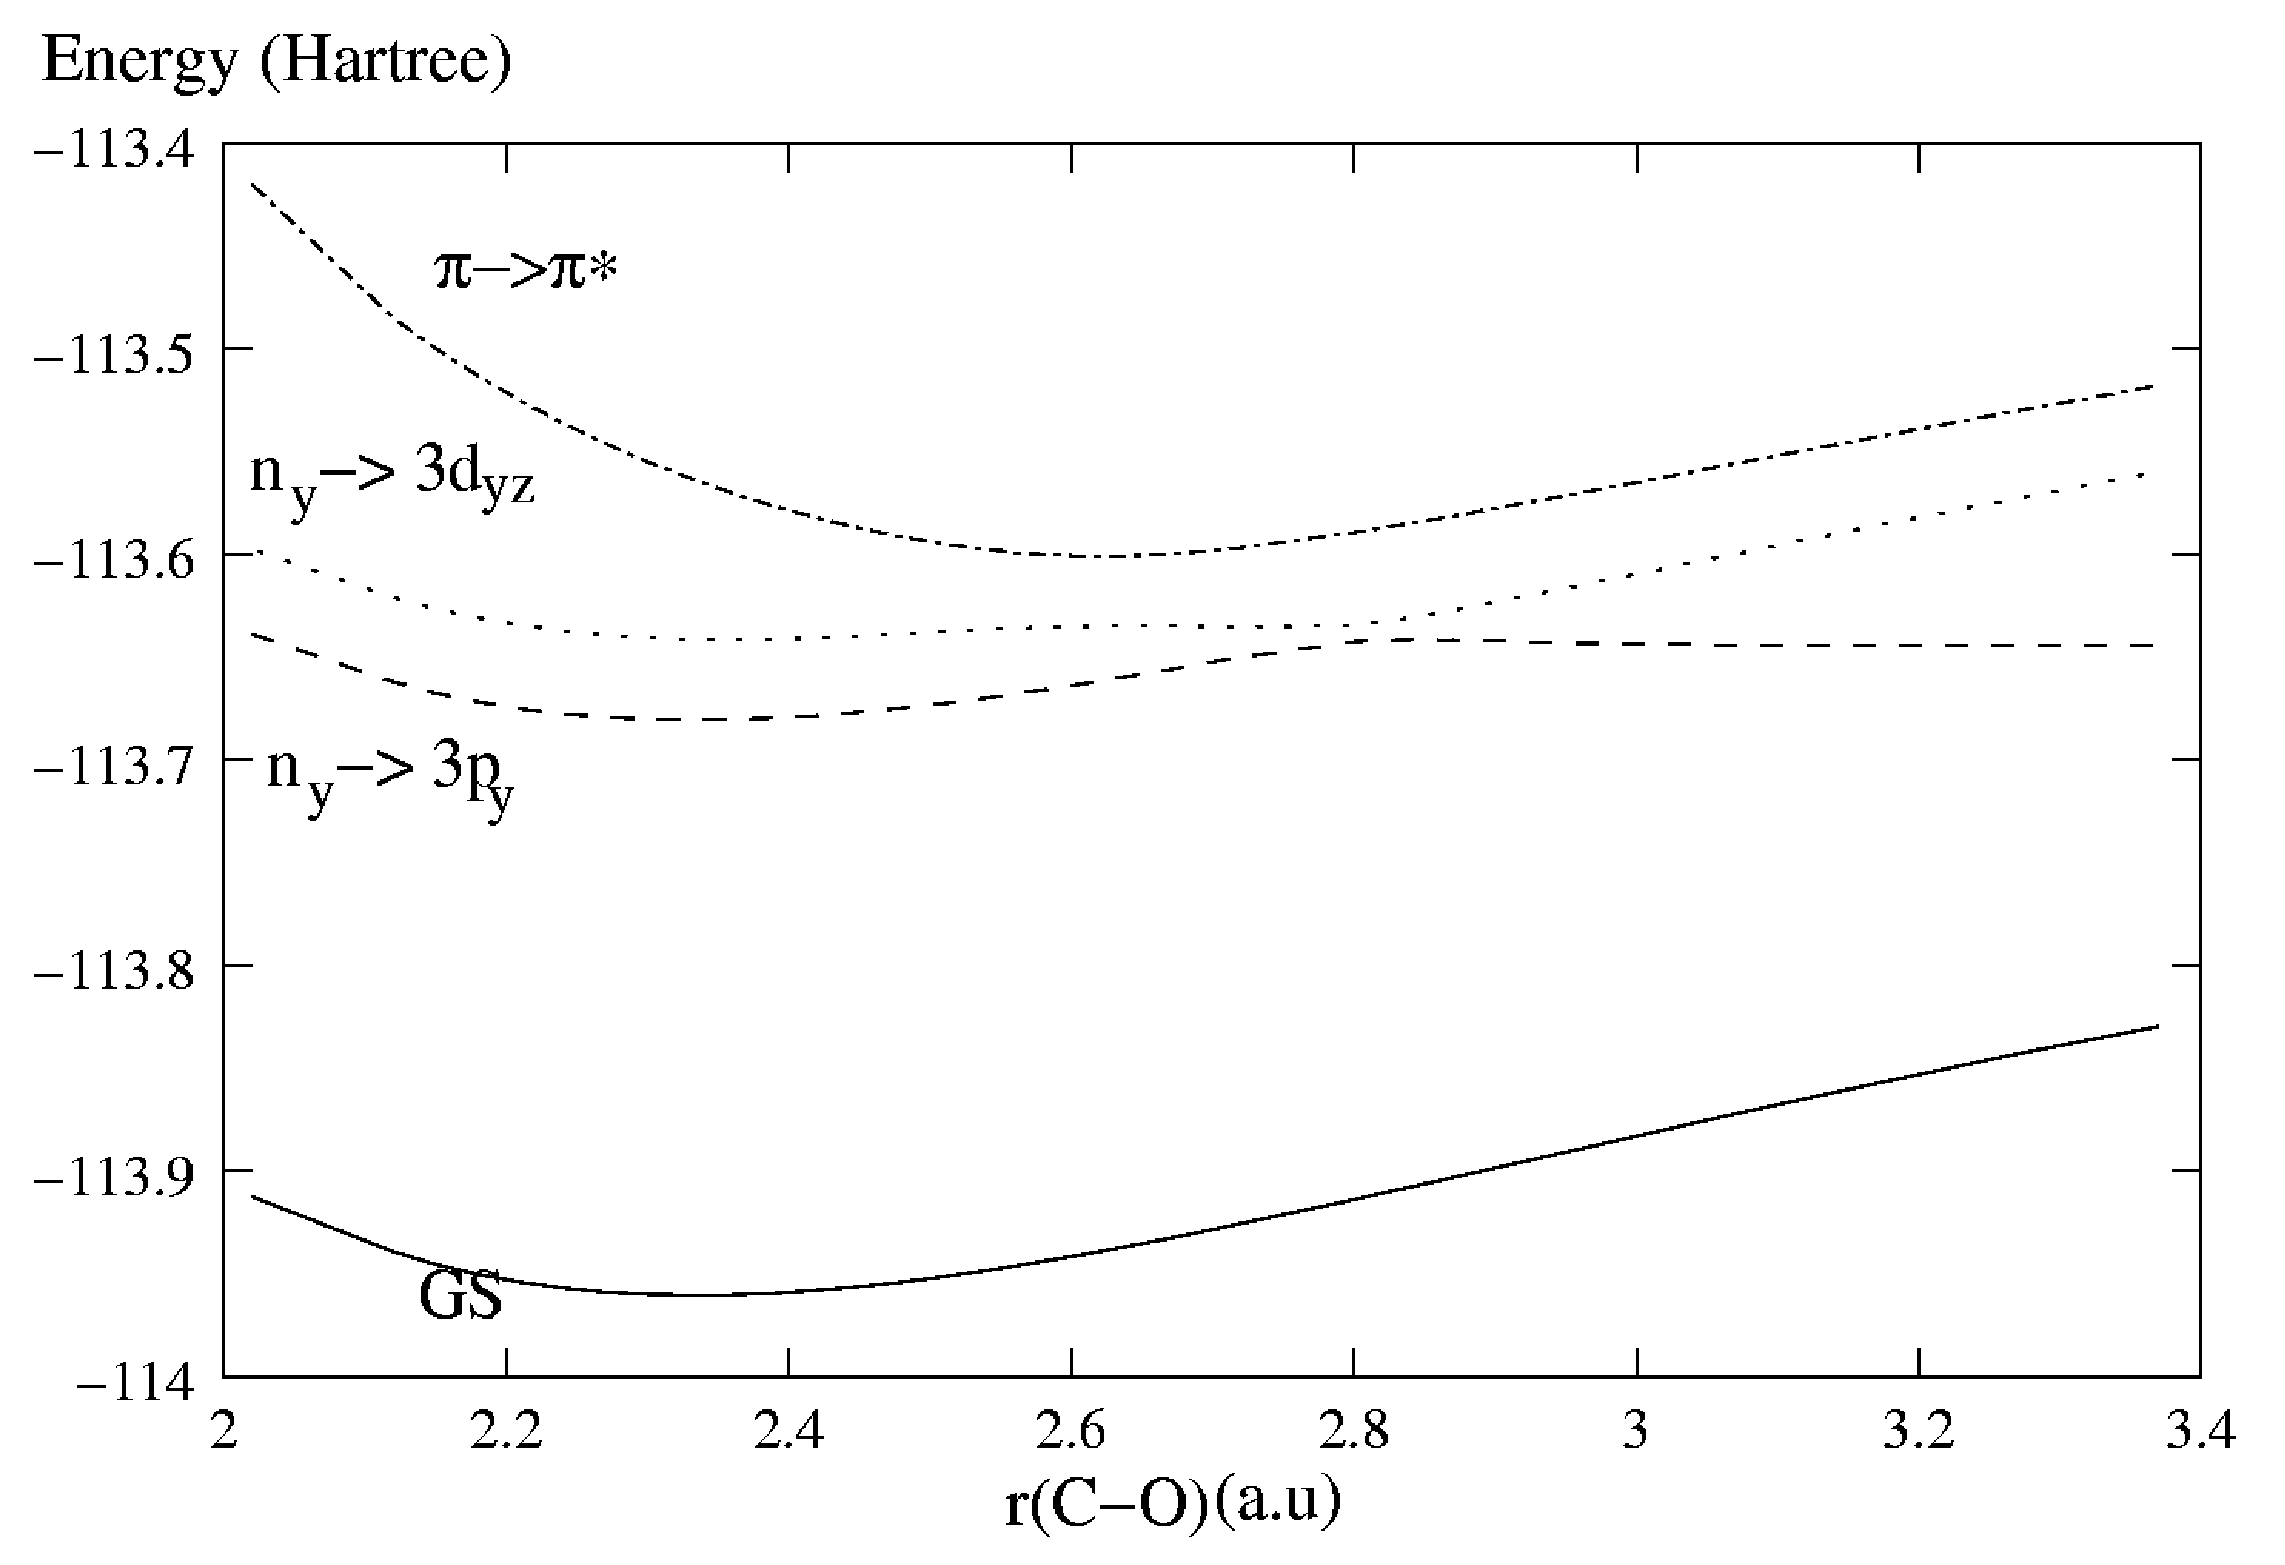
\includegraphics[width=11cm,keepaspectratio]{03_nevpt/images/formaldehyde-cas-curve.eps}
\end{center}
\caption{\footnotesize CASSCF energy curves for the ground state, $n \rightarrow$
Rydberg and $\pi \rightarrow \pi^{*}$ of formaldehyde with respect to the CO
bond lenght.}
\label{fig:formaldehyde_cas_curve}
\end{figure}
\end{center}

Applying the perturbation treatment, it is expected that the correlation for
valence states will be higher than for Rydberg states. 
As a direct consequence the avoided crossings move at shorter distances, see
Fig.~\ref{fig:formaldehyde_qdpt_curve}, solid line. The same plot also
reports the results produced by a Single-State NEVPT2 treatment (dotted
lines). These curves have no physical meaning and behave in incorrect ways.
The presence of non-diagonal elements in the effective Hamiltonian matrix
fixes the invalid behavior, allowing the wavefunction to interact at NEVPT2
level.
\vspace{-3mm}
\begin{center}
\begin{figure}[ht]
\begin{center}
\includegraphics[width=11cm]{03_nevpt/images/formaldehyde-qdpt-curve.eps}
\end{center}
\caption{\footnotesize Energy curves for the ground state, $n \rightarrow$
Ryd and $\pi \rightarrow \pi^{*}$ of formaldehyde with respect to the CO
bond lenght. The solid line represents the QD-NEVPT evaluation. The dotted
lines report the Single-State evaluation.}
\label{fig:formaldehyde_qdpt_curve}
\end{figure}
\end{center}

\vspace{-3mm}
A final consideration must however be raised working with a more accurate
point grid. The plot in Fig. \ref{fig:qdpt_error} represents the 2A$_1$ and
3A$_1$ Rydberg states at QD-NEVPT level of theory, using a finer grid (step
0.01 bohr) between 2.7 bohr and 2.9 bohr. An incorrect behavior is observed
for both curves. This behavior is not appreciable in the Ground
State and $\pi \rightarrow \pi^{*}$ curves. For comparison, the avoided
crossing at CASSCF level is reported between the QDPT curves. The CASSCF
curves have been transposed in energy to fit correctly into the plot.

It can be noted that the position of the incorrect behavior matches the
position of the avoided crossings at CASSCF level. This is probably due to a
wrong estimation of the coupling between the curves. Tests performed with
larger CAS spaces lead to a reduction of the incorrect behavior, which
expresses itself at shorter distances, following again the avoided crossing.
A possible explanation of the problem lies in a bad description of the
zero-order situation, and the inability for the NEVPT2 treatment to fully
recover the coupling. This brings a ``memory-effect'' on the QDPT curves.  A
non trivial solution to the problem could be looked for in the definition of an
iterative procedure, where the QD-NEVPT treatment is performed on the
refined wavefunctions obtained from the previous step. 
\vspace{-3mm}
\begin{center}
\begin{figure}[ht]
\begin{center}
\includegraphics[width=7cm,keepaspectratio,angle=270]{03_nevpt/images/qdpt_error.eps}
\end{center}
\caption{\footnotesize The incorrect behavior of the 2A$_1$ (cross symbol)
and 3A$_1$ (star symbol) Rydberg states at QD-NEVPT level, with respect to
the elongation of the CO bond. A grid step of 0.01 bohr between 2.7 and 2.9
bohr has been used.
Between the curves the plot also depicts the CASSCF avoided crossing taking
place at the same bond length. The avoided crossing curves have been
transposed to better fit into the plot. } \label{fig:qdpt_error}
\end{figure}
\end{center}

\vspace{-6mm}


%non canonical
\section{Non Canonical NEVPT}

All the cases so far examined of NEVPT were performed assuming canonical
orbitals, since the situation is greatly simplified using these orbitals.
Let us consider the inactive part of the Dyall's Hamiltonian in generalized form
\beqa
\ham^D_i &=& \sumidx{ij} f_{ij} E_{ij} + \sumidx{rs} f_{rs} E_{rs}
\eeqa
where the $f_{xy}$ elements are relative to the Fock matrix on a CASSCF
wavefunction $\Psi_0$
%\beq
%f_{xy} = \half \sum_{\sigma=\alpha,\beta}
%\braket{\Psi_0}{\anticomm{\constr{y\sigma}}{\comm{\destr{x\sigma}}{\ham}}
%}{\Psi_0}
%\eeq
\beq
f_{xy} = - \braket{\Psi_0}{\constr{x} \comm{\ham}{\destr{y}}}{\Psi_0} +
\braket{\Psi_0}{\destr{x} \comm{\ham}{\constr{y}}}{\Psi_0}
\eeq
Diagonalization of $\ham^D$ is simplified if we assume that
canonical orbitals are used and the inactive part is cast as the
well-known diagonal case
\beqa
\ham^D_i &=& \sumidx{i} \epsilon_{i} E_{ii} + \sumidx{r} \epsilon_{r} E_{rr}
\eeqa
The simplification arises by the fact that the perturber energies are
defined by a simple quantity. For example, we recall the case for the S$^0$
class where the energy of the perturber $E_{ri} E_{sj} \Psi_m^{(0)}$ is
$E_m^{(0)} + \epsilon_r + \epsilon_s - \epsilon_i -\epsilon_j$. This
obviously cannot be obtained quickly if non-canonical orbitals are used.

A solution resides in a different evolution of the first-order perturbation
equation:
\beq
\left( \ham^{(0)} - E_m^{(0)} \right) \Psi_m^{(1)} = \left( E_m^{(1)} - \hat{V} \right) \Psi_m^{(0)}
\eeq
Instead of expressing the $\Psi_m^{(1)}$ as a linear combination of the
zero-order wavefunctions
\beq
\Psi_m^{(1)} = \sumidx{k}c_k \Psi_k^{(0)}
\eeq
we develop using generic functions $\Phi_l$
\beq
\Psi_m^{(1)} = \sumidx{l}c_l \Phi_l
\eeq
A system of linear equations must be solved
\beq
\sum_l c_l \left[ \braket{\Phi_k}{\ham_0}{\Phi_l} - E_m^{(0)}
\integral{\Phi_k}{\Phi_l} \right] = - \braket{\Phi_k}{\hat{V}}{\Psi_m^{(0)}}
\eeq
\beq
E_m^{(2)} = \braket{\Psi_m^{(0)}}{\hat{V}}{\Psi_m^{(1)}} = \sum_l c_l
\braket{\Psi_m^{(0)}}{\hat{V}}{\Phi_l}
\eeq
using the internally contracted $E_{wx} E_{yz} \Psi_m^{(0)}$ as $\Phi_l$.

%Once deployed the linear system of equations, it can be cast in the form
%\beq
%\left(\mathbf{1} - \mathbf{A} \right) \mathbf{x} = \mathbf{x}_0
%\eeq
%FIXME : spiegare i simboli
%and solved iteratively by building a set of vectors $\mathbf{x}_0$,
%$\mathbf{x}_1$, $\ldots$, $\mathbf{x}_k$ given by
%\beq
%\mathbf{x}_{n+1} = \mathbf{A} \mathbf{x}_{n} - \sum_{l=0,n}
%\frac{\braket{\mathbf{x}_{l}}{A}{\mathbf{x}_{n}}}{\integral{\mathbf{x}_{l}}{\mathbf{x}_{l}}}
%\mathbf{x}_{l}
%\eeq
%It is now possible to optimize the $\alpha_k$ coefficients of the vector
%$\mathbf{x} = \sum_k \alpha_k \mathbf{x}_{k}$ by minimizing the square norm
%of the error vector
%\beq
%\integral{\left(\mathbf{1} - \mathbf{A} \right) \mathbf{x} -
%\mathbf{x}_0}{\left(\mathbf{1} - \mathbf{A} \right) \mathbf{x} -
%\mathbf{x}_0}
%\eeq

\section{NEVPT and Localization}

A first successful integration of localization and NEVPT2 has been deployed
to show the feasibility of this approach.
An acetone molecule and two water molecules coordinating the CO oxygen have
been optimized at 6-311G*/MP2 level. The molecular system has C$_{2v}$
geometrical symmetry, and the CH$_3$ groups have been rotated to feature
on-plane hydrogens far from one another. The symmetry has been considered
only during geometry optimization, while for the rest of the evaluation the
C$_1$ symmetry group has been used to work with non-symmetric localized
orbitals.

A minimal atomic basis set ANO-1 with $2s1p$ contraction for heavy atoms, and
$1s$ for hydrogen has been used. From this basis, a set of localized orbitals
is obtained with the procedure presented in Sec.
\ref{sec:toulouse_method}. These orbitals are optimized by means of a
Super-CI based optimization chain, converging to a localized CASSCF
solution. An active space comprising six electrons in five
active orbitals ($\sigma$, $\sigma^{*}$, $\pi$, $\pi^{*}$ of the acetone
carbonyl group, and the $n_y$ lone pair of the carbonyl oxygen) has been
defined. The active orbitals are visible in Fig. \ref{fig:h2o-active}

\begin{center}
\begin{figure}[ht]
\begin{center}
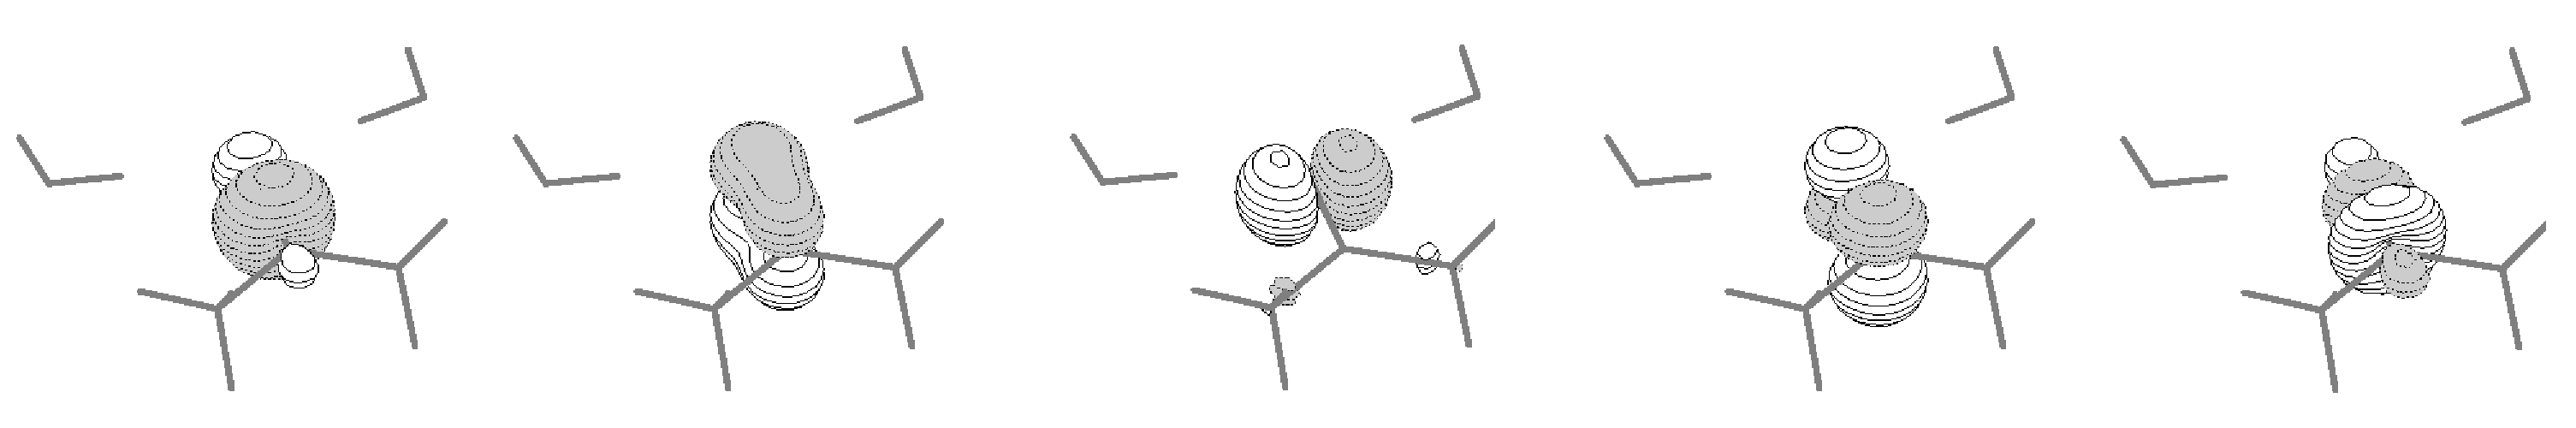
\includegraphics[width=11cm]{03_nevpt/images/h2o-active.eps}
\end{center}
\caption{\footnotesize The active orbitals for the evaluation on Acetone + 2
H$_2$O. From left to right, the $\sigma$, $\pi$, $n_y$, $\pi^{*}$,
$\sigma^{*}$. }
\label{fig:h2o-active}
\end{figure}
\end{center}


These orbitals are used in a Single-State NEVPT2 and a Non-Canonical
procedure, leading to the perturbative results presented in the left side
of Tab.~\ref{tbl:noncanonical}.  

\begin{center}
\begin{threeparttable}
\footnotesize
\begin{tabular*}{\textwidth}{l@{\hspace*{27mm}}cccc}
\hline
        & \multicolumn{2}{c}{Non-canonized} & \multicolumn{2}{c}{Canonized} \\
        &  SS-NEVPT     &  NC-NEVPT     &  SS-NEVPT     &  NC-NEVPT     \\
\hline
        &    \multicolumn{4}{c}{Ground State}\\
  (0)   & -0.1562219292 & -0.1610160883 & -0.1610160655 & -0.1610160655 \\
  (+1)  & -0.0060289124 & -0.0063728566 & -0.0063728572 & -0.0063728572 \\
  (-1)  & -0.0083210019 & -0.0084680922 & -0.0084680918 & -0.0084680918 \\
  (+2)  & -0.0021959738 & -0.0022262691 & -0.0022262691 & -0.0022262691 \\
  (-2)  & -0.0012134175 & -0.0011964952 & -0.0011964953 & -0.0011964954 \\
  (+1)' & -0.0011298902 & -0.0010747735 & -0.0010747734 & -0.0010747734 \\
  (-1)' & -0.0081324857 & -0.0080043857 & -0.0080043841 & -0.0080043842 \\
  (0)'  & -0.0095463813 & -0.0099518340 & -0.0099518346 & -0.0099518346 \\
\hline                                 
Total   & -0.1927899918 & -0.1983107946 & -0.1983107710 & -0.1983107711 \\
\hline                                 
        &    \multicolumn{4}{c}{\snpi}\\
\hline
  (0)   & -0.1569058671 & -0.1616113655 & -0.1616113419 &  -0.1616113419 \\
  (+1)  & -0.0089370064 & -0.0093753612 & -0.0093753625 &  -0.0093753624 \\
  (-1)  & -0.0059930216 & -0.0061061218 & -0.0061061209 &  -0.0061061209 \\
  (+2)  & -0.0009248766 & -0.0009503478 & -0.0009503479 &  -0.0009503479 \\
  (-2)  & -0.0002921853 & -0.0002913366 & -0.0002913366 &  -0.0002913366 \\
  (+1)' & -0.0043652467 & -0.0046995715 & -0.0046995705 &  -0.0046995704 \\
  (-1)' & -0.0025446880 & -0.0025151544 & -0.0025151554 &  -0.0025151554 \\
  (0)'  & -0.0117850231 & -0.0123542659 & -0.0123542653 &  -0.0123542652 \\
\hline
Total   & -0.1917479149 & -0.1979035247 & -0.1979035010 &  -0.1979035008 \\
\hline
\end{tabular*}
\caption{\footnotesize Comparison between the obtained contributions for the non-canonical technique.
The ``Non-canonized'' columns show the values obtained with non-canonical
localized orbitals using Partially Contracted Single-State NEVPT (SS-NEVPT)
and Non-Canonical NEVPT (NC-NEVPT).
The ``Canonized'' columns report the same evaluations, where a preliminar 
canonization of the localized orbitals has been performed. Both SS-NEVPT and
NC-NEVPT confirm the values obtained in the Non-canonized NC-NEVPT
evaluation.\label{tbl:noncanonical}
}
\end{threeparttable}
\end{center}

\vspace{4mm}

As can be seen, a non-negligible difference is present
between the obtained values.  Standard single-state NEVPT2 supposes the
non-diagonal elements of the Fock matrix as zero.  The \texttt{dypcNC}
program provides the highest non-diagonal element of the core and virtual
Fock matrixes

{
\footnotesize
\begin{verbatim}
 Maximum of off-diagonal core Fock matrix is   0.238695436106739
 Maximum of off-diagonal virtual Fock matrix is   8.252258688390988E-002
\end{verbatim}
}
which can be appreciated as non zero. This results in an error of the single
state treatment. 

The Non-Canonical evaluation keeps into account the non
diagonality of the Fock matrix, producing the correct value.
The correctness of this result is confirmed by canonizing the optimized
orbitals right before the perturbative evaluation. In this case, the
localization is lost, but the \texttt{dypcNC} confirms the diagonality of
the Fock matrix

{
\footnotesize
\begin{verbatim}
 Maximum of off-diagonal core Fock matrix is   6.924101073191773E-008
 Maximum of off-diagonal virtual Fock matrix is   4.398960914047209E-008
\end{verbatim}
}
and the obtained results (right side of Tab. \ref{tbl:noncanonical})
confirm the value obtained with the first evaluation.

A plot of the different nature of the orbitals used in the evaluation can be
seen in Fig. \ref{fig:h2o-orb}. The upper part of the figure shows an
extract of the localized set of non canonical orbitals, while the lower part plots
an extract of the orbitals after canonization. The delocalization of the
orbitals is clearly appreciable. 

\begin{center}
\begin{figure}[ht]
\begin{center}
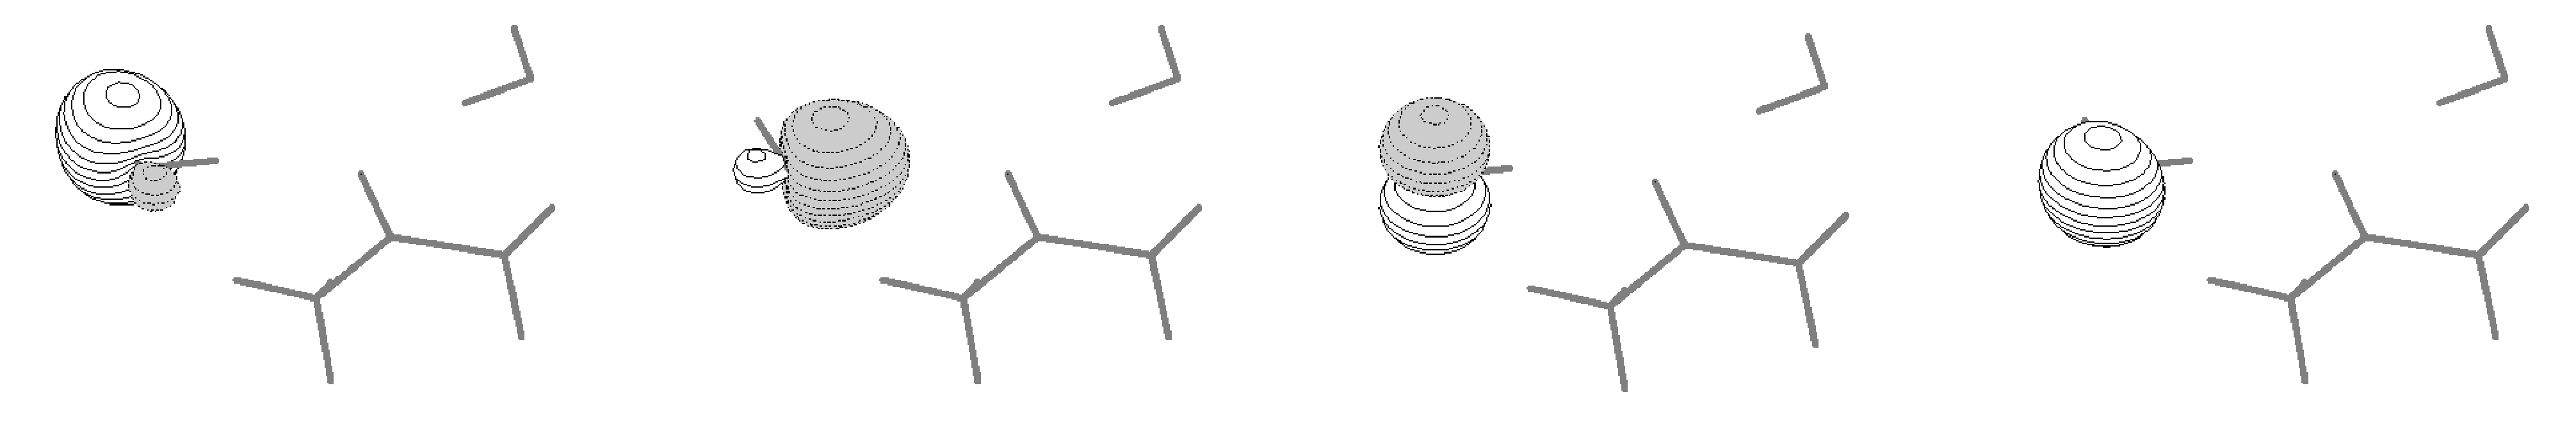
\includegraphics[width=11cm]{03_nevpt/images/h2o-loc.eps}
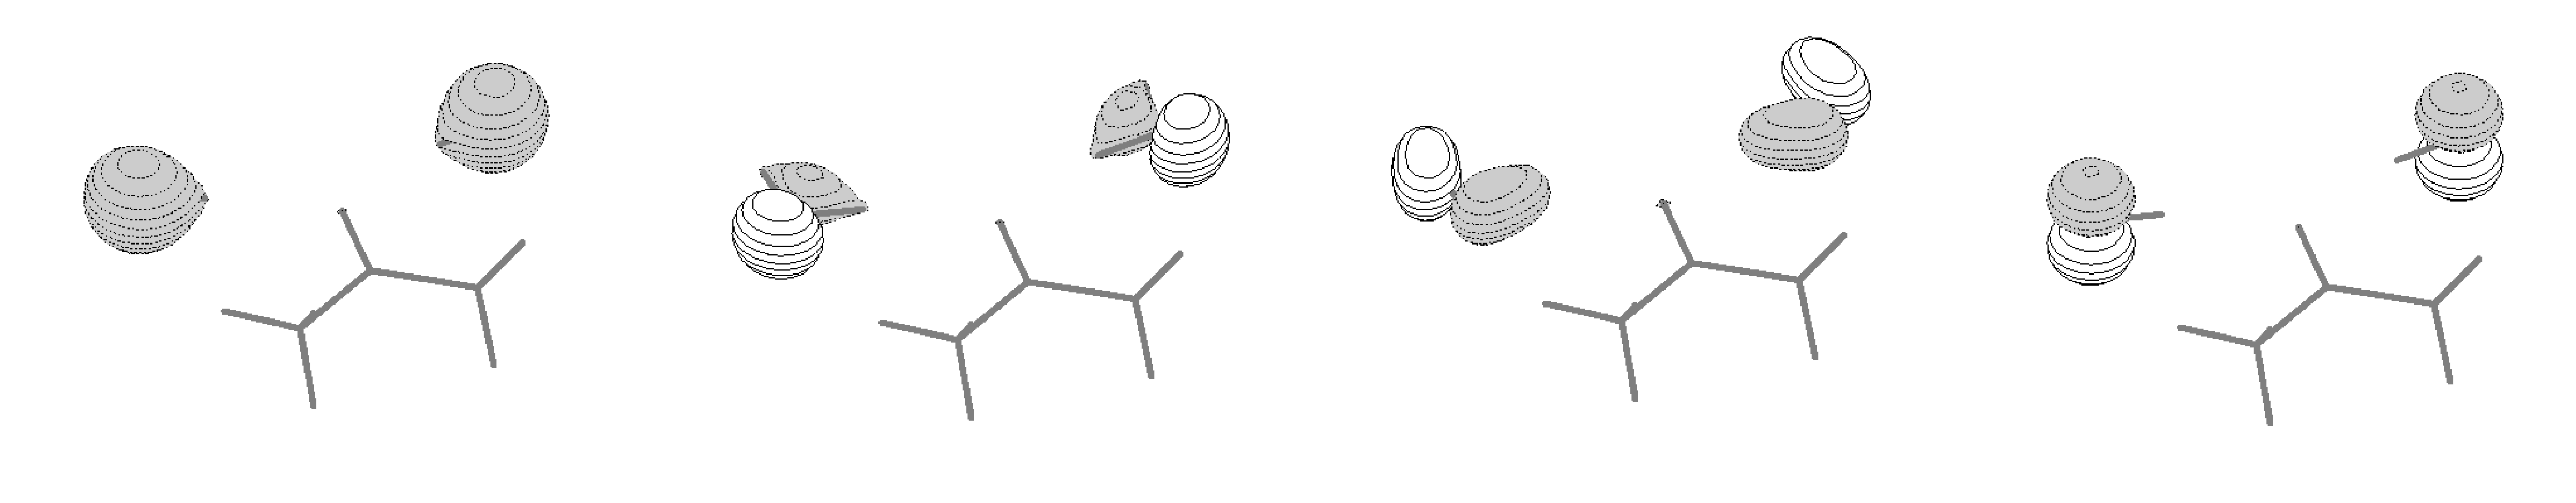
\includegraphics[width=11cm]{03_nevpt/images/h2o-deloc.eps}
\end{center}
\caption{\footnotesize A sample plot of non canonical localized orbitals
(upper part of the figure) and canonical delocalized orbitals (lower part)
for water orbitals. }
\label{fig:h2o-orb}
\end{figure}
\end{center}


Evaluating the energy difference provides consistency of the results.  For
the reported test, no high difference in the relative energies can be found,
as can be seen in Tab. \ref{tbl:noncanonical_energy}.

\begin{center}
\begin{threeparttable}
\begin{tabular*}{0.80\textwidth}{l@{\hspace*{27mm}}cccc}
\hline
        &  Ground   &  Excited    & Diff. \\
\hline
CASSCF   & -343.573883 & -343.411249 & 4.42 \\
SS-NEVPT & -343.766673 & -343.602997 & 4.45 \\
NC-NEVPT & -343.772194 & -343.609153 & 4.43 \\
\hline                                 
\end{tabular*}
\caption{\footnotesize Absolute energies and their differences for the
acetone+2 H$_2$O system. From the comparison of the relative excitation
energies, no high differencies between the methods can be found in the
analyzed system.
}
\label{tbl:noncanonical_energy}
\end{threeparttable}
\end{center}


This must be further investigated, given the small basis set used. However,
the target of this investigation was to demonstrate the consistency of the
NC-NEVPT results.



